\chapter{Dark matter multivariate analysis}
\label{app:mva}

\section{Boosted decision trees}

The multivariate analysis makes use of the implementation of boosted decision trees (BDTs) in the TMVA software package within the ROOT framework \cite{Hocker:2007ht}.

A decision tree is a binary tree structured classifier.
Repeated yes/no decisions are taken on a single variable at a time until a stop criterion is fulfilled.
The phase space is split this way into many regions that are eventually classified as signal or background, depending on the majority of training events that end up in the final leaf node.

The boosting of a decision tree extends this concept from one tree to several trees which form a forest. 
The trees are derived from the same training ensemble by reweighting events, and are finally combined into a single classifier which is given by a weighted average of the individual decision trees. 
Boosting stabilizes the response of the decision trees with respect to fluctuations in the training sample and is able to considerably enhance the performance with respect to a single tree. 

\subsection{Gradient boosting}
The idea of function estimation through boosting can be understood by considering a simple additive expansion approach.
Consider a particular point $\vec{\mathbf{x}}$ in the space of variables describing the dataset.
The function $F(\vec{\mathbf{x}})$ under consideration is assumed to be a weighted sum
of parameterized base functions or \textit{weak learners} $f(\vec{\mathbf{x}};\:a_m)$.
Each base function corresponds to a decision tree
\begin{equation}
F(\vec{\mathbf{x}}) = \sum_{m=0}^{M} \beta_m f(\vec{\mathbf{x}};\:a_m)\qquad P\in\{\beta_m;\:a_m\}^M_0
\end{equation}
where $M$ is the number of trees in the forest, $m$ represents a particular decision tree,
and $P$ is the parameter space of tree weights $\beta_m$ and tree decisions $a_m$.

The boosting procedure adjusts the parameters $P$ so that the deviation between the model response
$F(\vec{\mathbf{x}})$ and the true value $y$ obtained from the training input data is minimized.
For the BDT classifier, the binomial log-likelihood loss function is used for the gradient boosting algorithm:
\begin{equation}
L(F,y) = \mathrm{ln}\left(1+e^{-2F(\vec{\mathbf{x}}) y}\right)
\end{equation}
The minimization is achbieved using an iterative gradient-descent approach.
The gradient of the loss function for the current forest, $F_{m-1}(\vec{\mathbf{x}})$, is calculated.
Then, a new decision tree $h_m(\vec{\mathbf{x}})$ is grown to match
the mean value of the gradient in each region defined by the tree structure.
A coefficient $\gamma_m$ is found via line search to get the new forest $F_m(\vec{\mathbf{x}})$
that minimizes the loss function:
\begin{equation}
F_m(\vec{\mathbf{x}}) = F_{m-1}(\vec{\mathbf{x}}) + \gamma_m \cdot h_m(\vec{\mathbf{x}})
\end{equation}
Iterating this procedure over several hundred trees yields the desired set of
decision trees which minimizes the loss function.

In general, gradient boosting is performed using regularization techniques 
to avoid overfitting the training data. Here, shrinkage and bagging are used.
These are described below.
The BDT seen in Chapter~\ref{chap:zlldm}, Section~\ref{sec:dmmva}
was grown with 400 trees, shrinkage parameter $\nu=0.5$, and bagging fraction 0.5.

\subsubsection{Shrinkage}
In the above description, the $m^{th}$ tree used to correct the classifier is directly added to the existing forest with coefficient $\gamma_m$.
That coefficient can be shrunk by a constant factor $\nu$ at each step of the iteration to slow the so-called ``learning rate.''
The update rule can be modified to reduce the weight of this addition:
\begin{equation}
F_m(\vec{\mathbf{x}}) = F_{m-1}(\vec{\mathbf{x}}) + \nu \cdot \gamma_m \cdot h_m(\vec{\mathbf{x}})
\end{equation}

With shrinkage, a more generalized model is attained.
But more trees are needed to solve the problem,
increasing the computational expense of training as well as evaluating the BDT.

\subsubsection{Bagging}
Random subsamples of the training data can be used for growing the trees. This is called bagging.
The bagging fraction is the fraction of training data randomly chosen for the iterations.

\section{Choice of input variables}

\begin{figure}[htbp]
\begin{center}
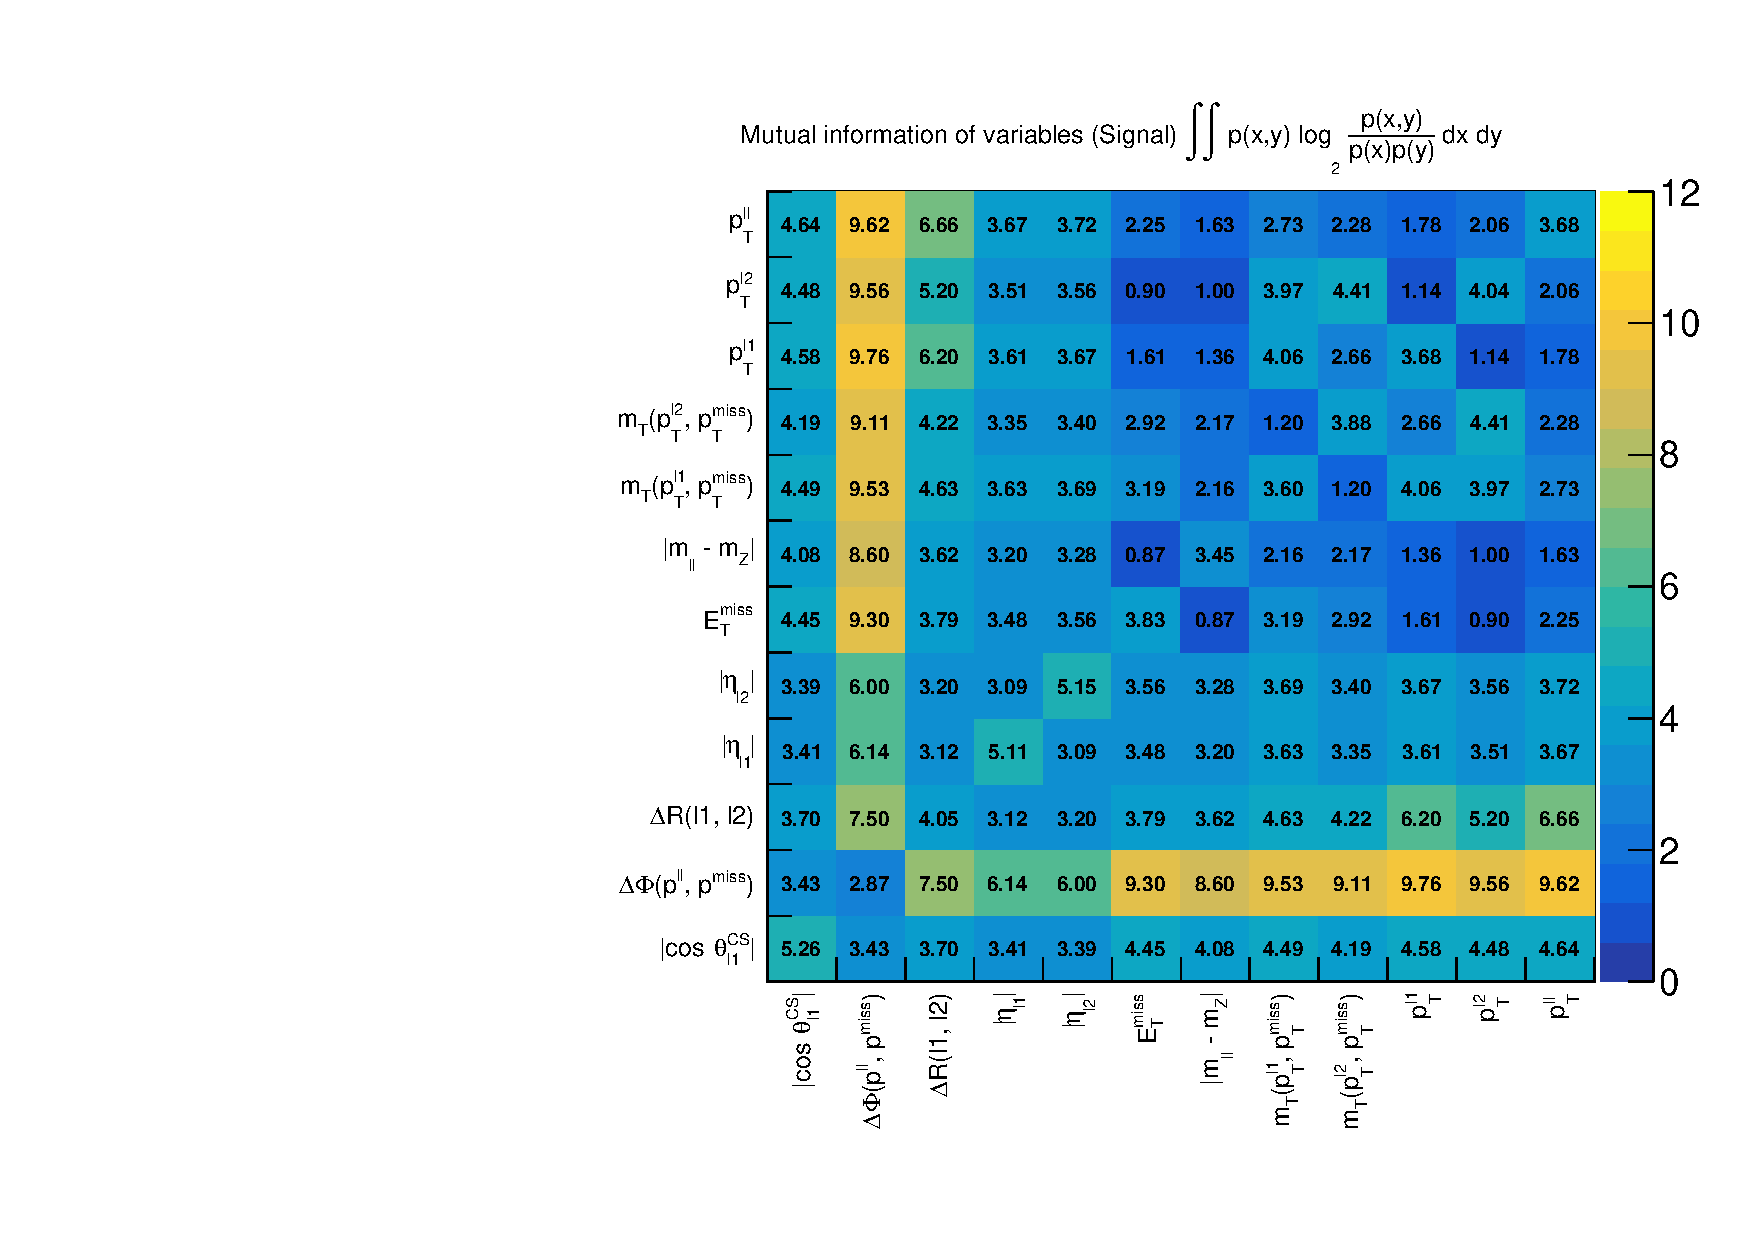
\includegraphics[width=0.48\textwidth]{figures/mutual_information_MVAvars_Signal.pdf}
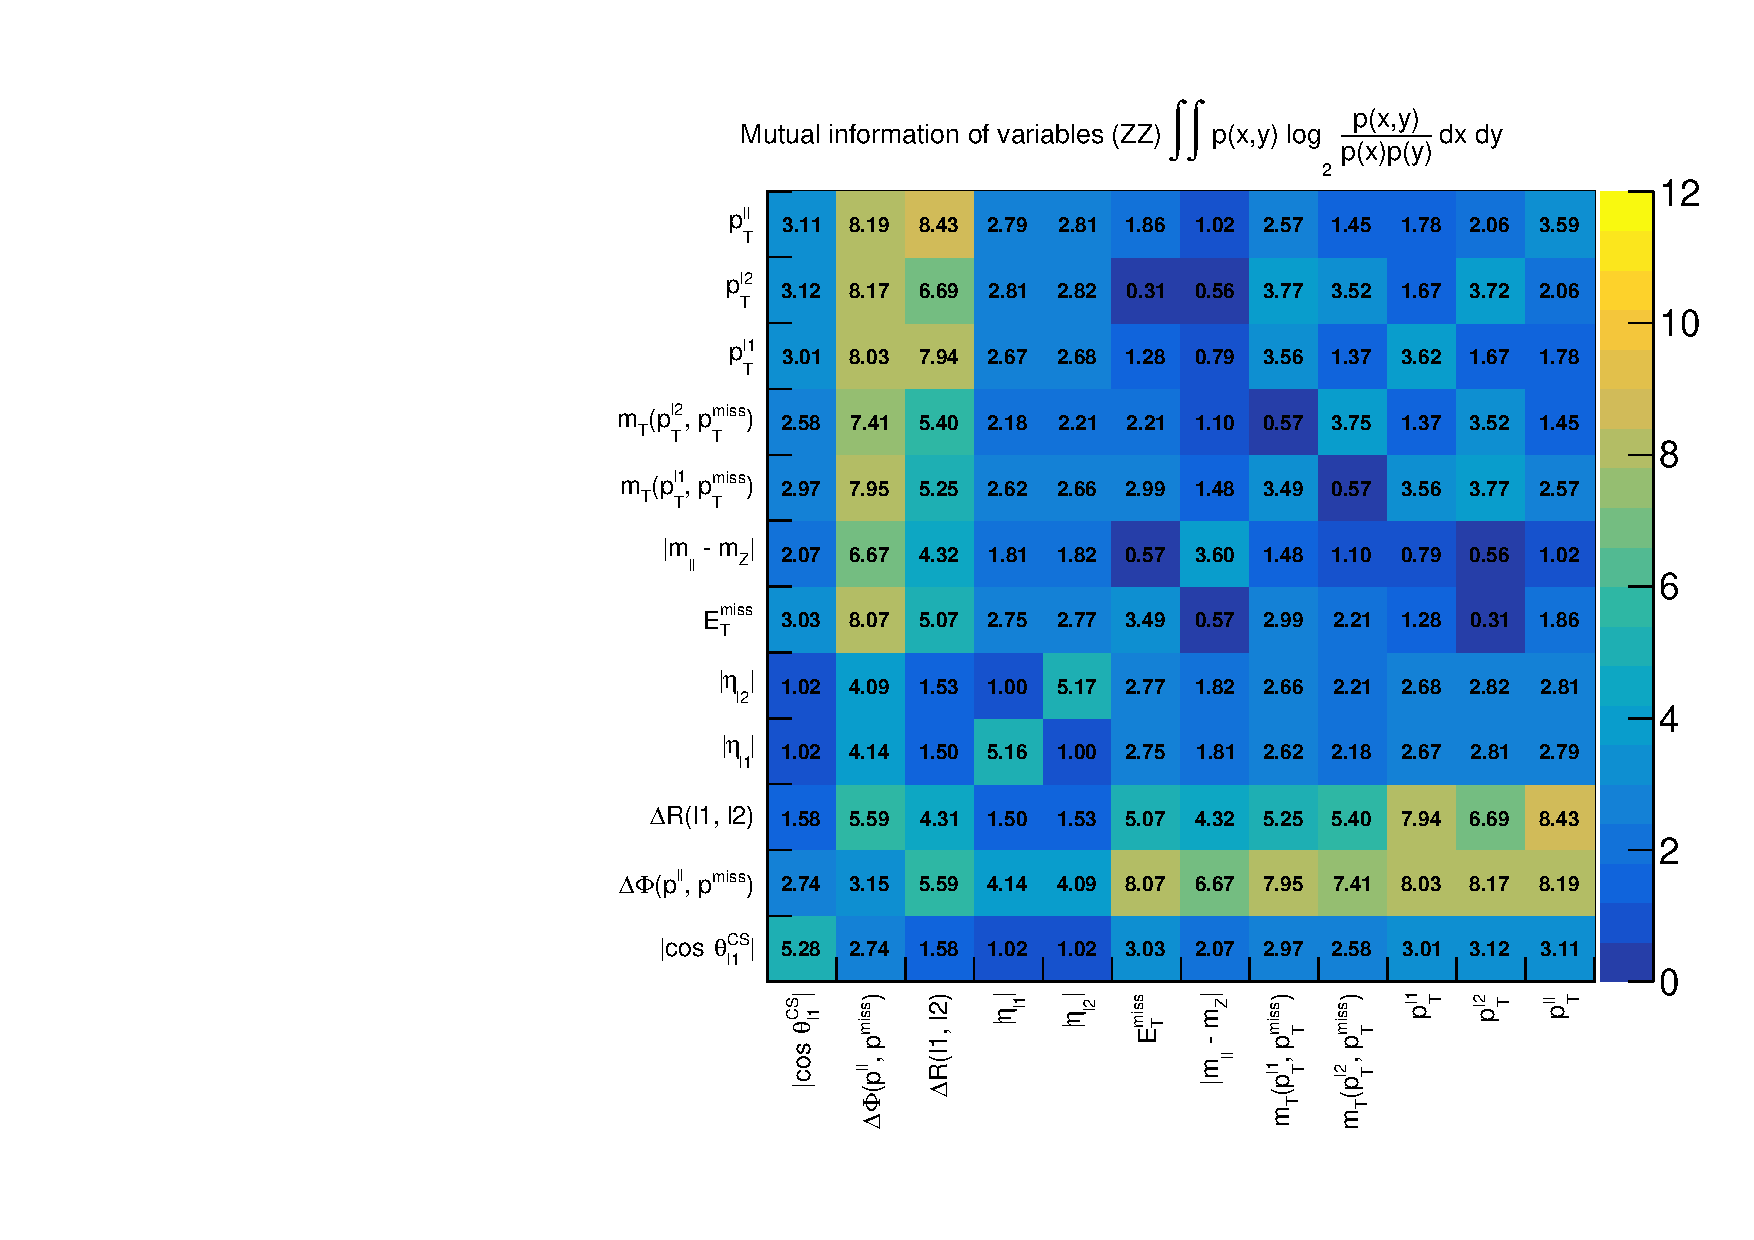
\includegraphics[width=0.48\textwidth]{figures/mutual_information_MVAvars_ZZ.pdf}
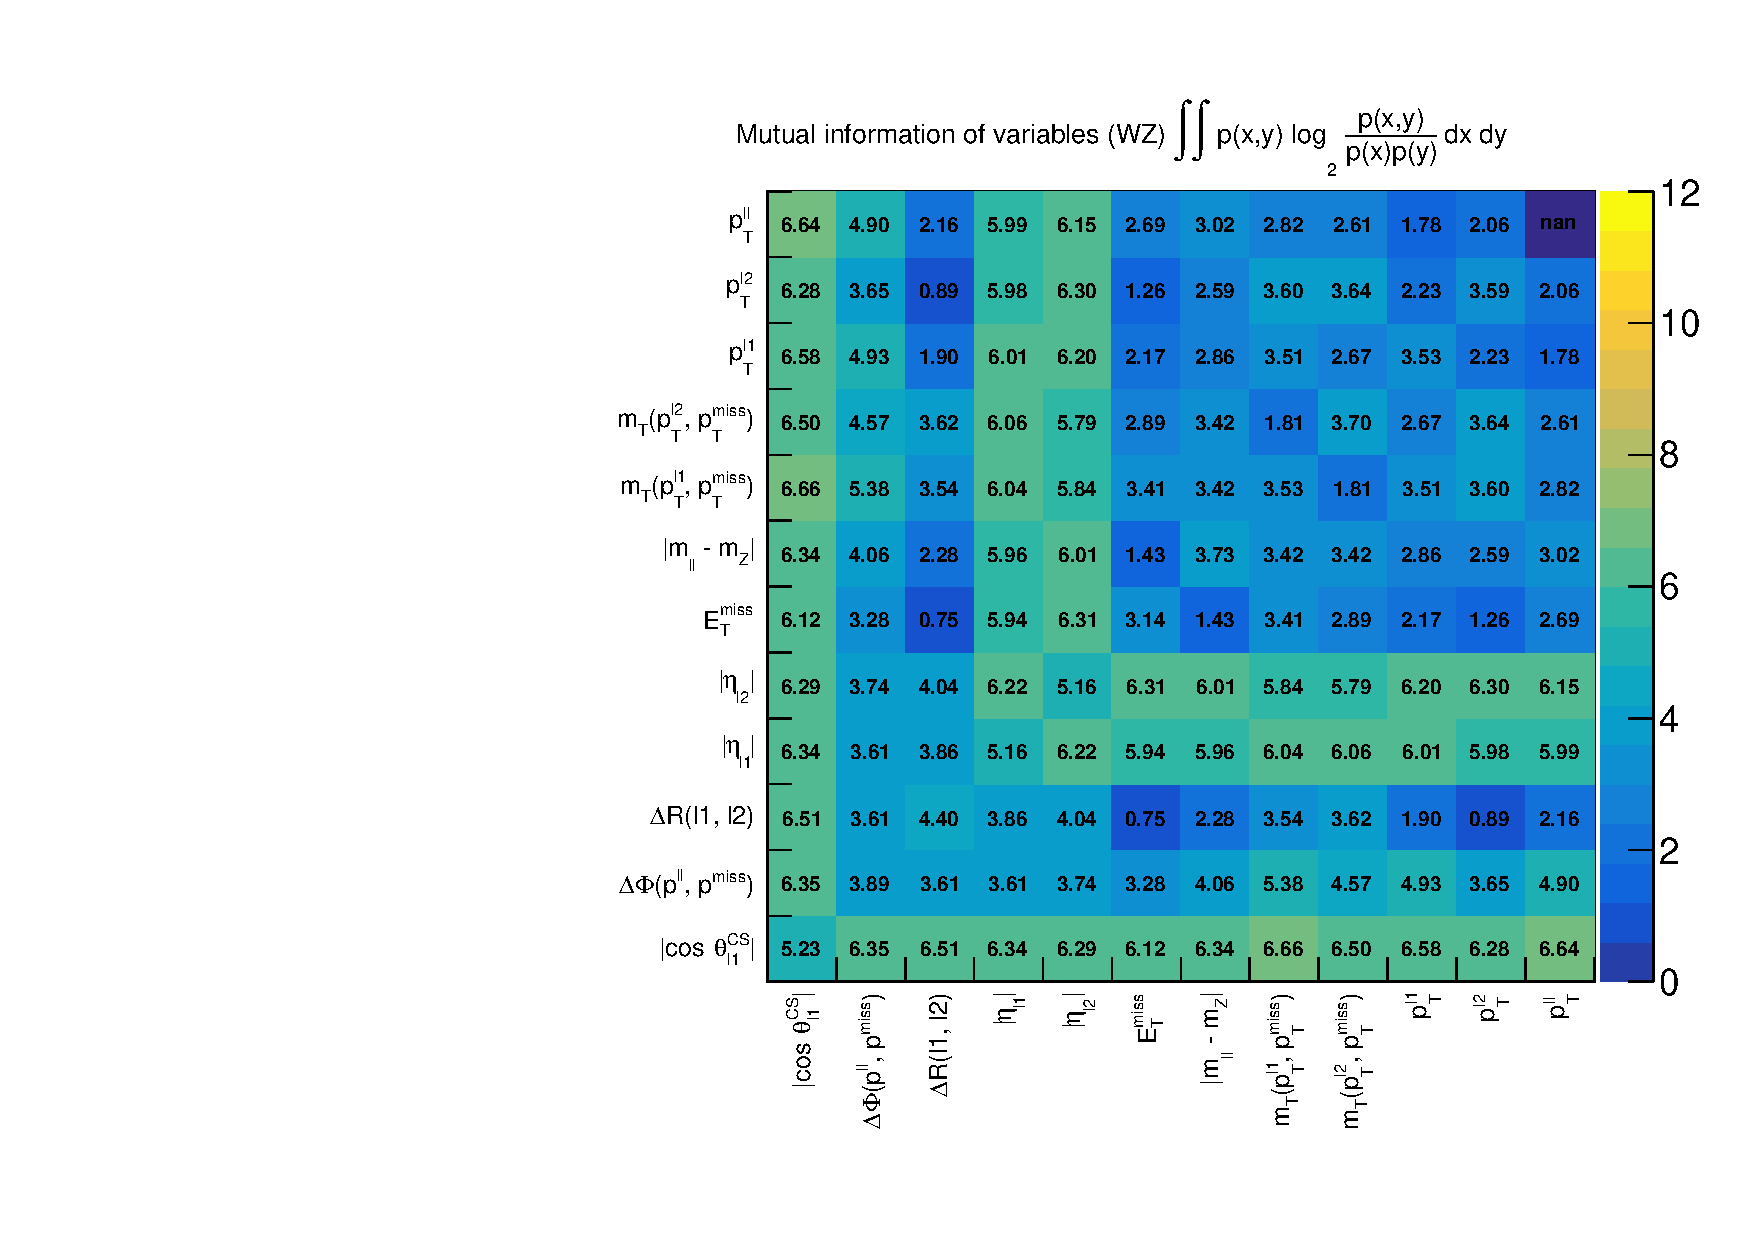
\includegraphics[width=0.48\textwidth]{figures/mutual_information_MVAvars_WZ.pdf}
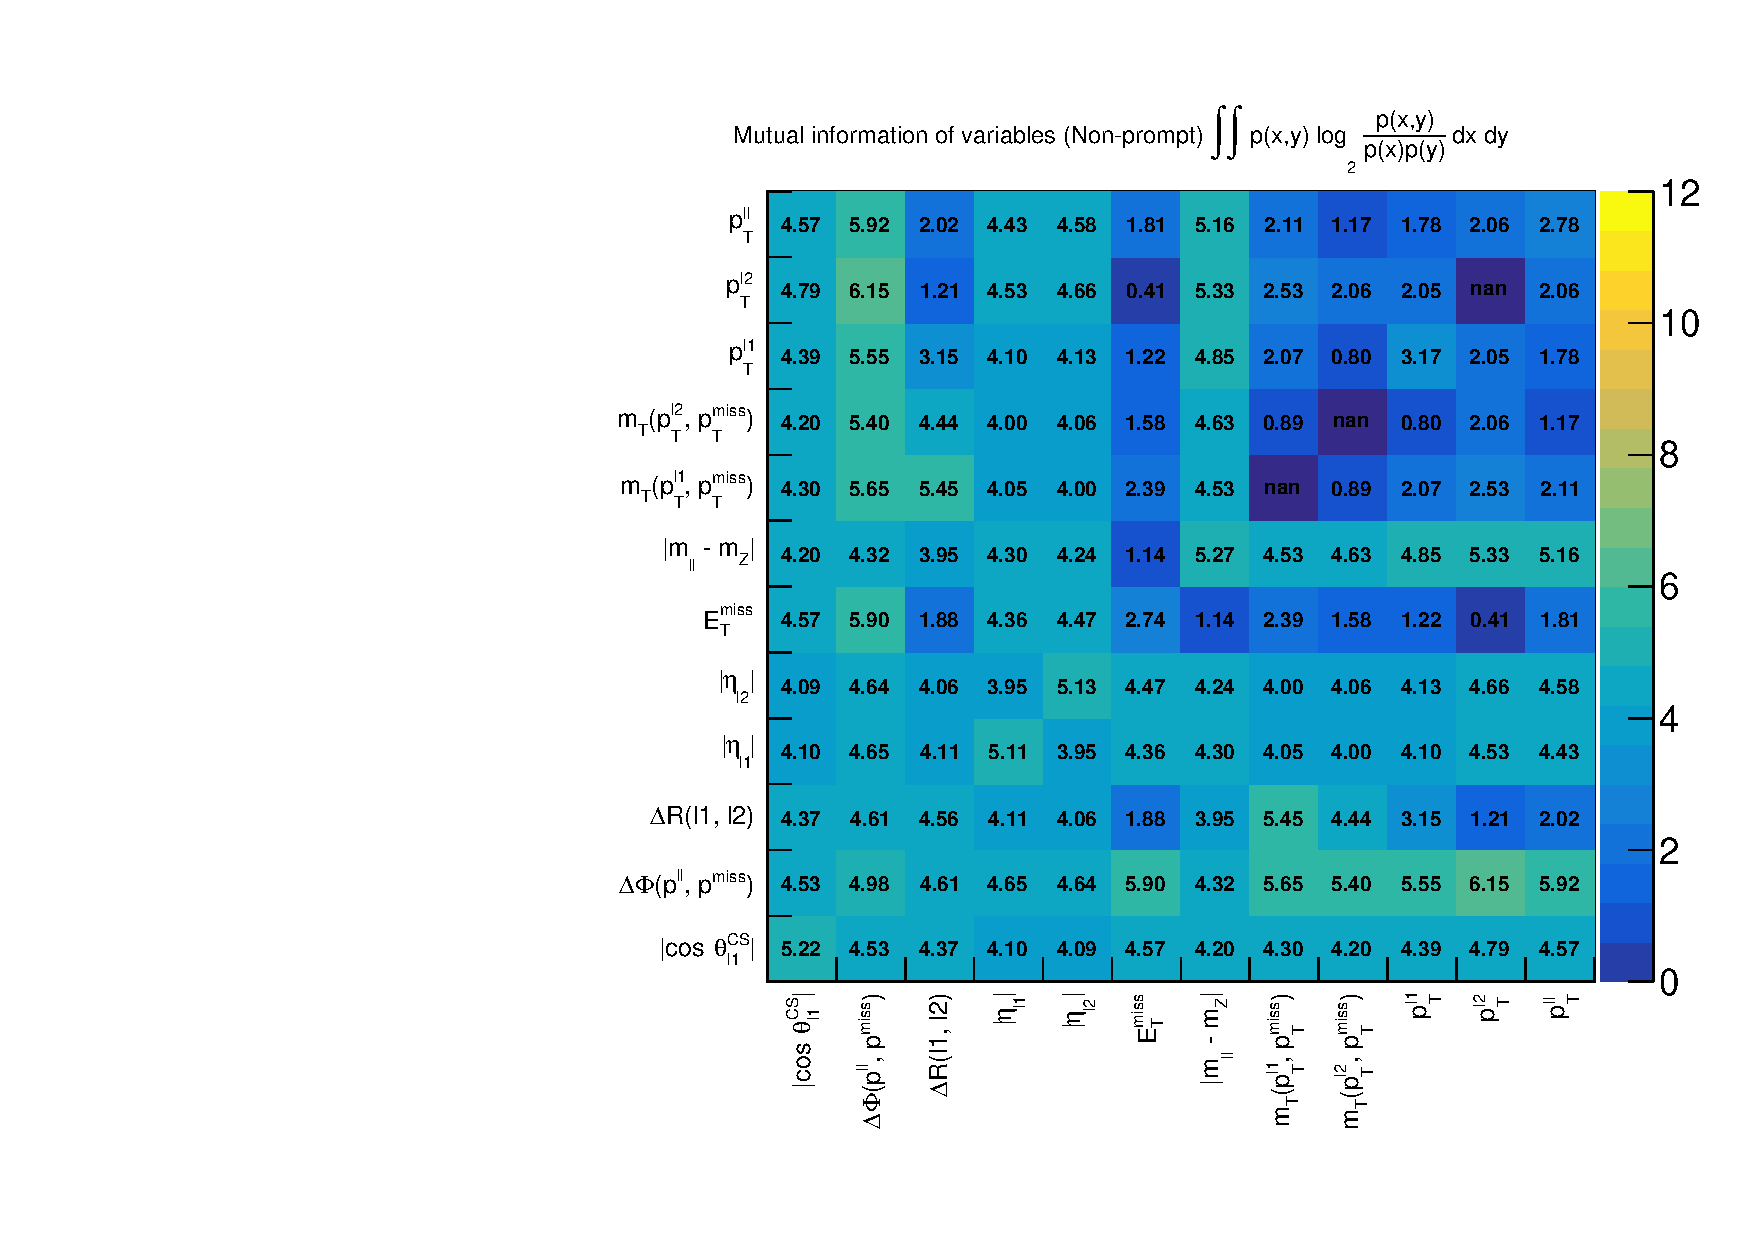
\includegraphics[width=0.48\textwidth]{figures/mutual_information_MVAvars_Non-prompt.pdf}
\caption{Mutual information between the twelve BDT input variables for the invisible Higgs, ZZ, WZ, and flavor-symmetric (non-prompt) classes. The matrix for the Drell-Yan class is statistically irrelevant.}
\label{fig:bdt_mutual_information}
\end{center}
\end{figure}

\begin{figure}[htbp]
\begin{center}
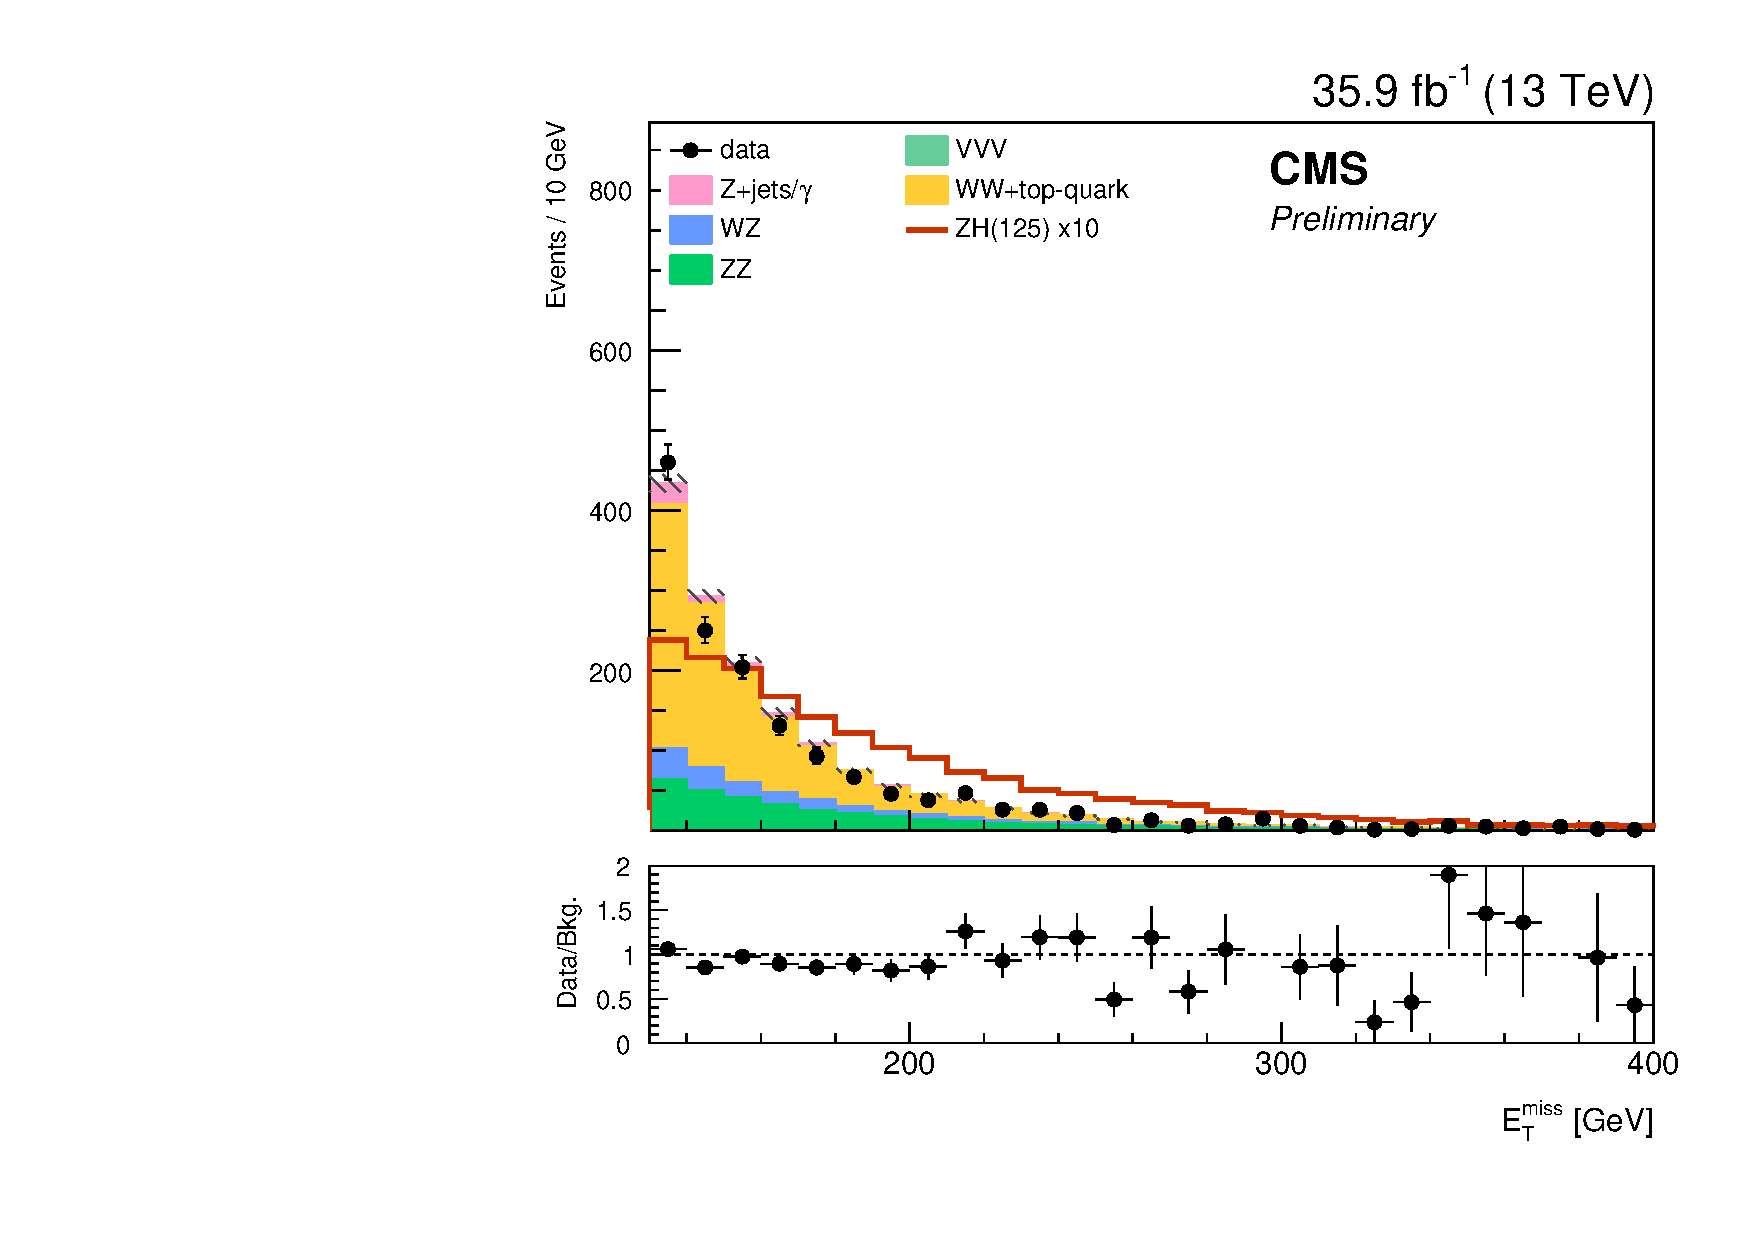
\includegraphics[width=0.48\textwidth]{figures/mva_MET_nice.pdf}
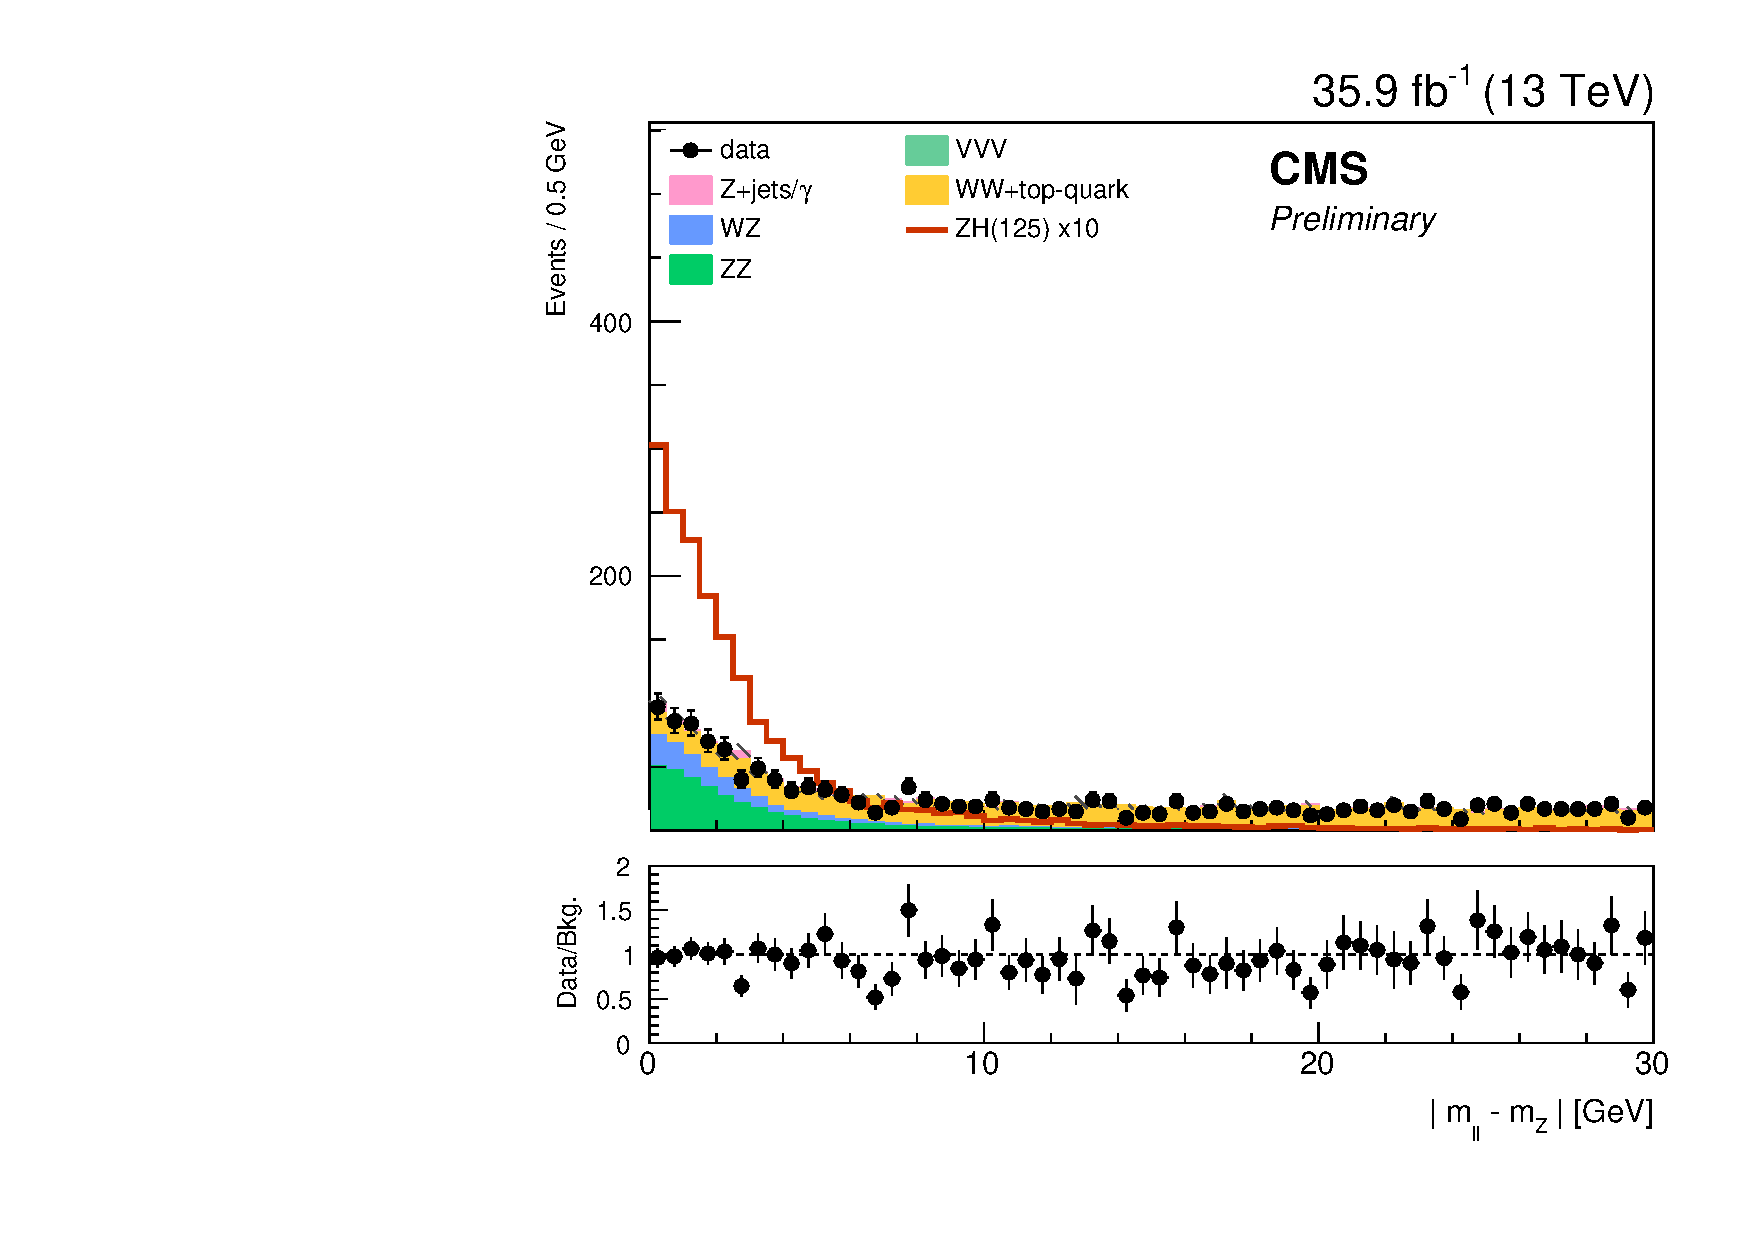
\includegraphics[width=0.48\textwidth]{figures/mva_mll_minus_mZ_nice.pdf}
%\includegraphics[width=0.48\textwidth]{figures/mva_balance_nice.pdf}
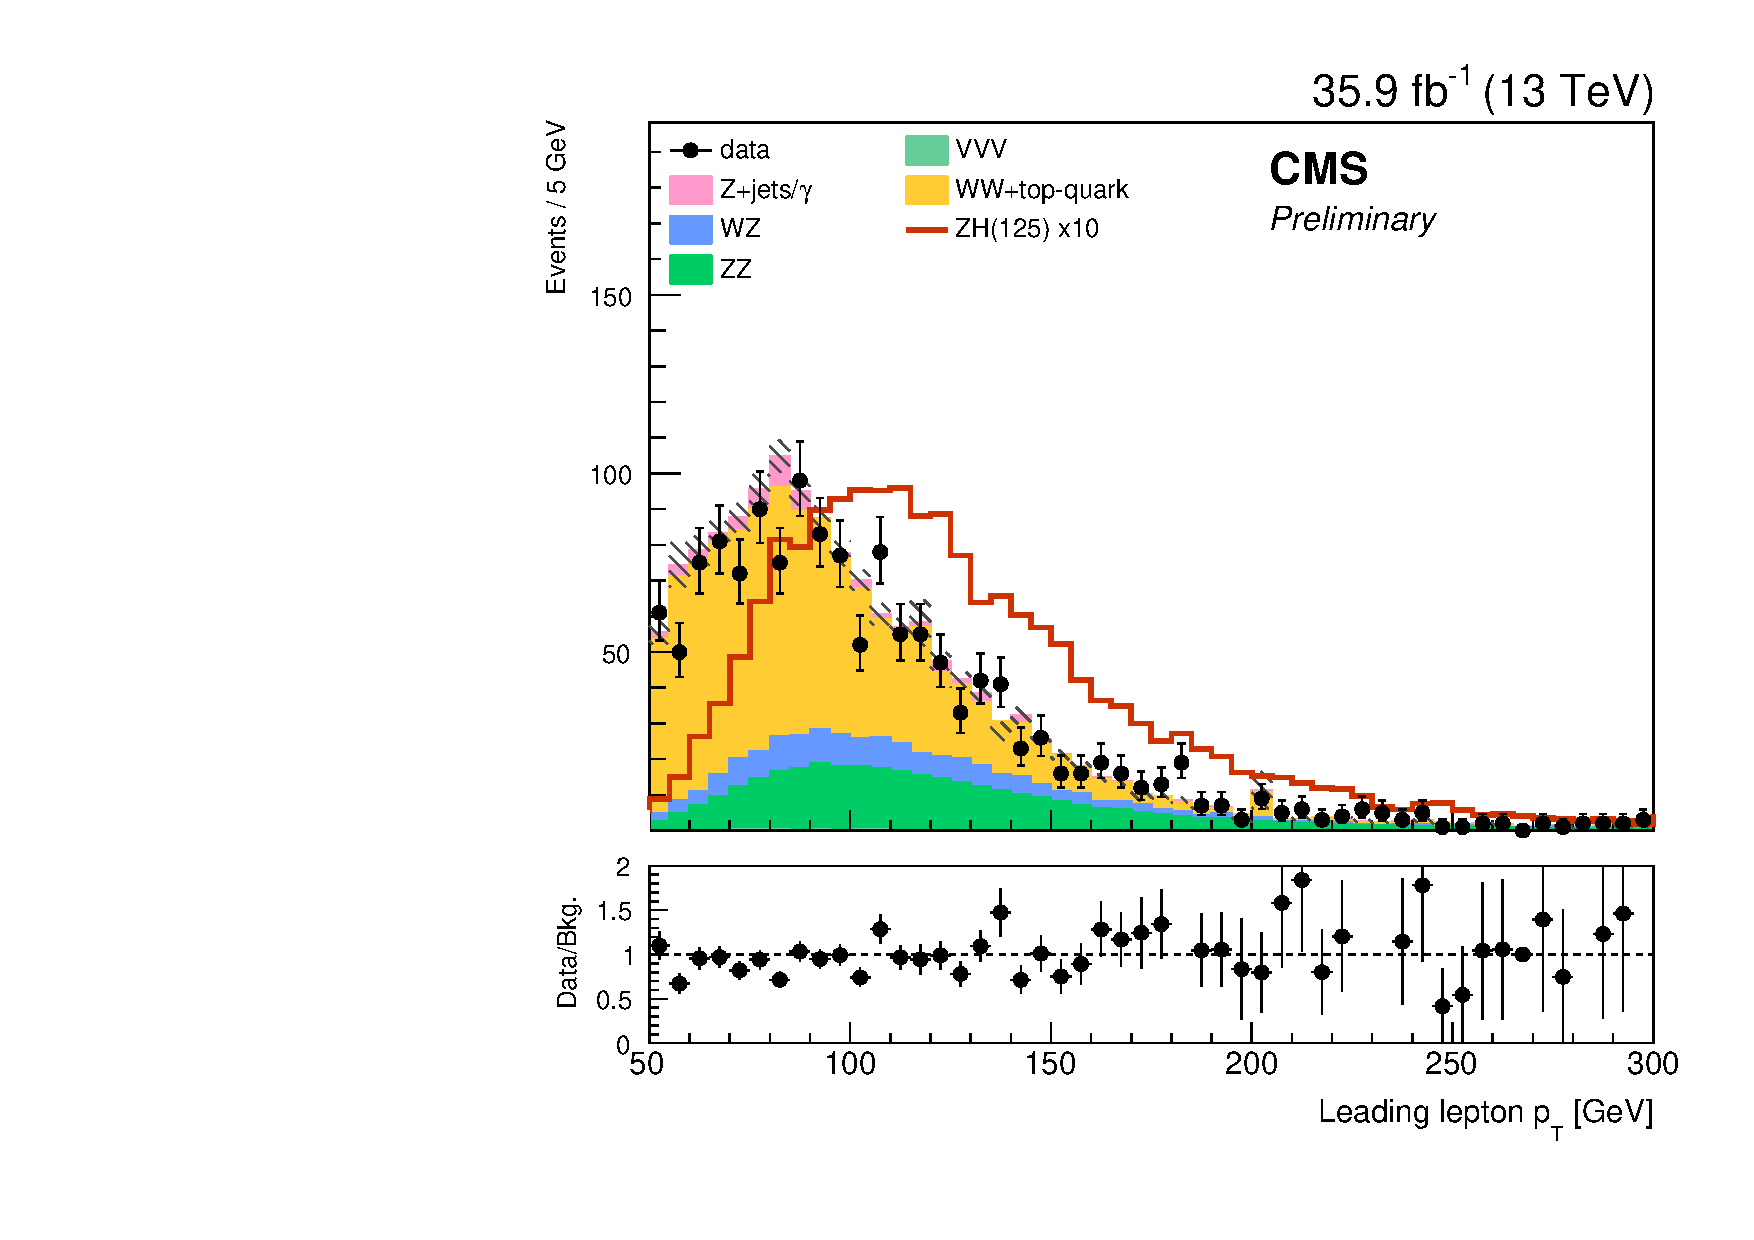
\includegraphics[width=0.48\textwidth]{figures/mva_ptl1_nice.pdf}
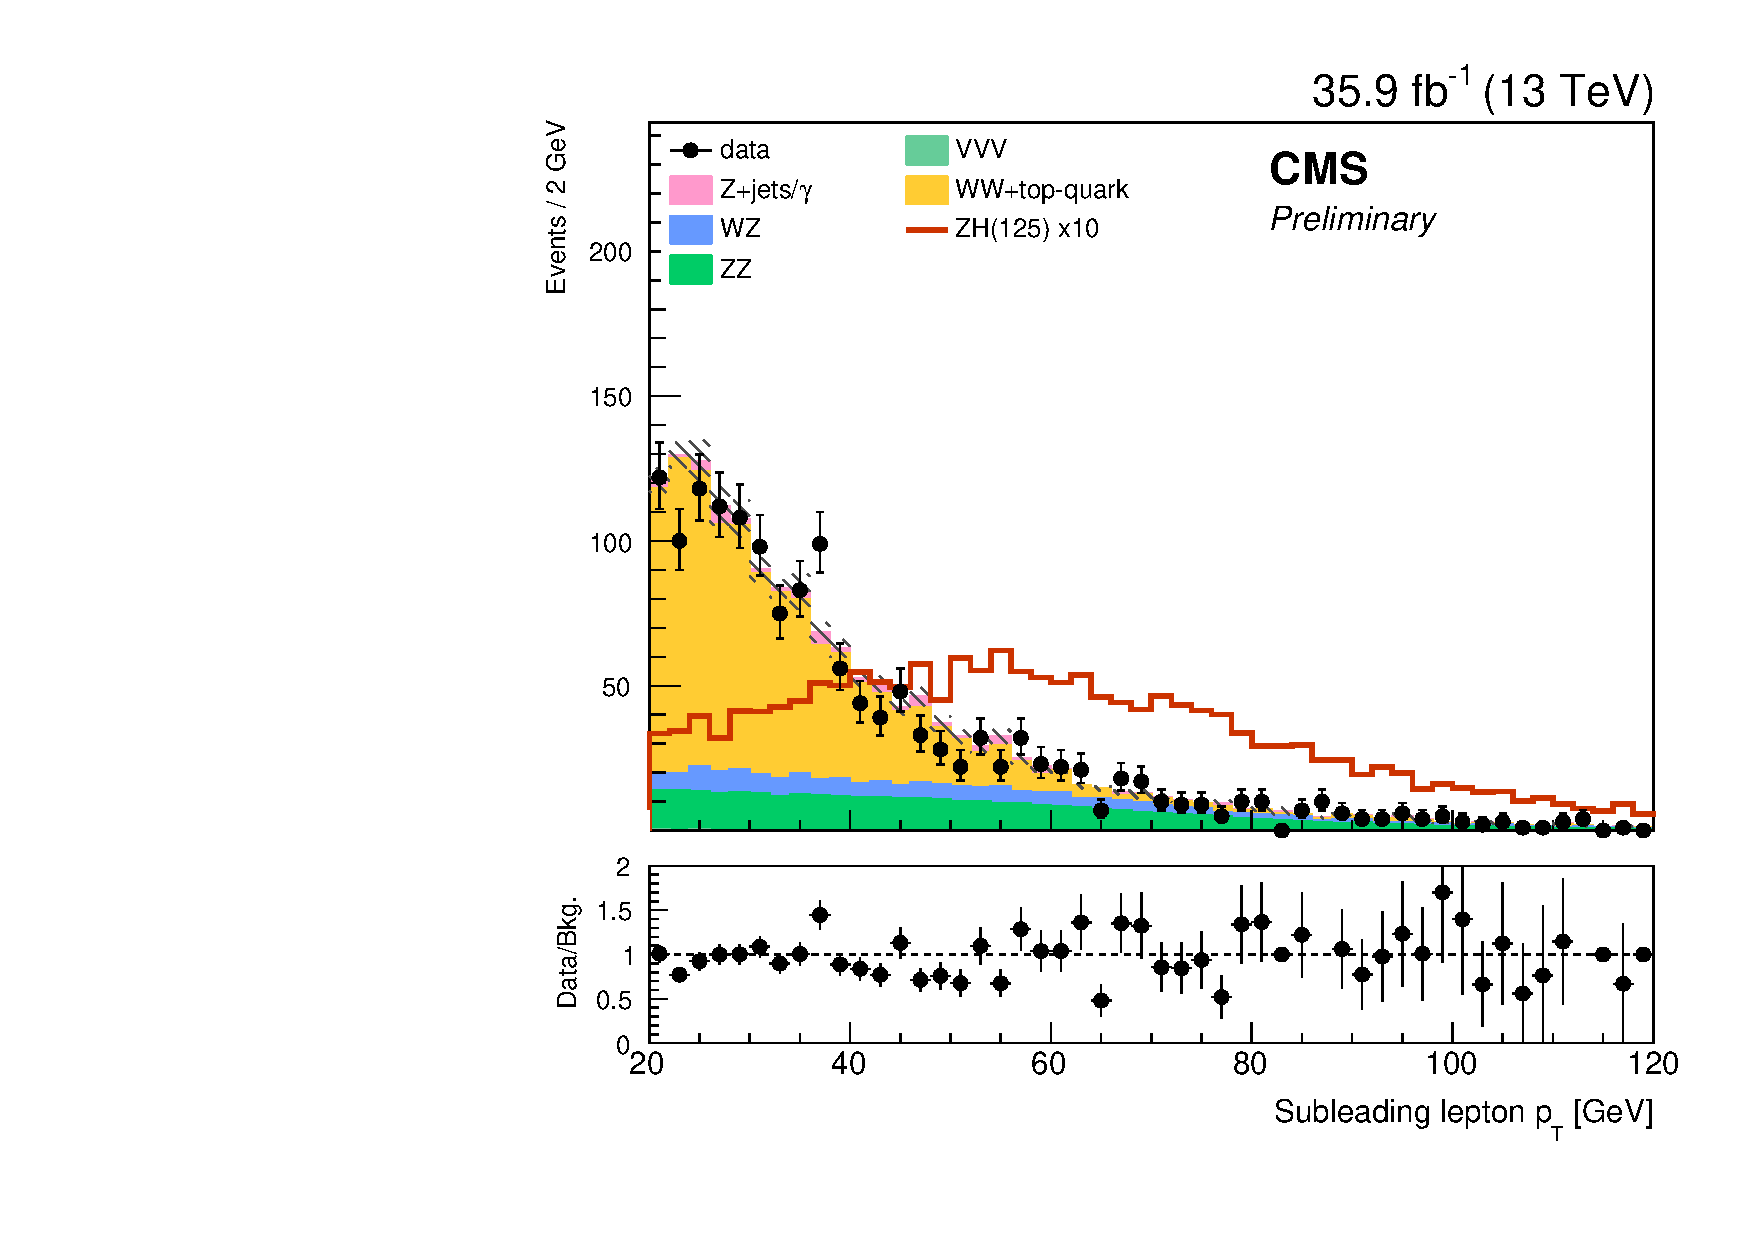
\includegraphics[width=0.48\textwidth]{figures/mva_ptl2_nice.pdf}
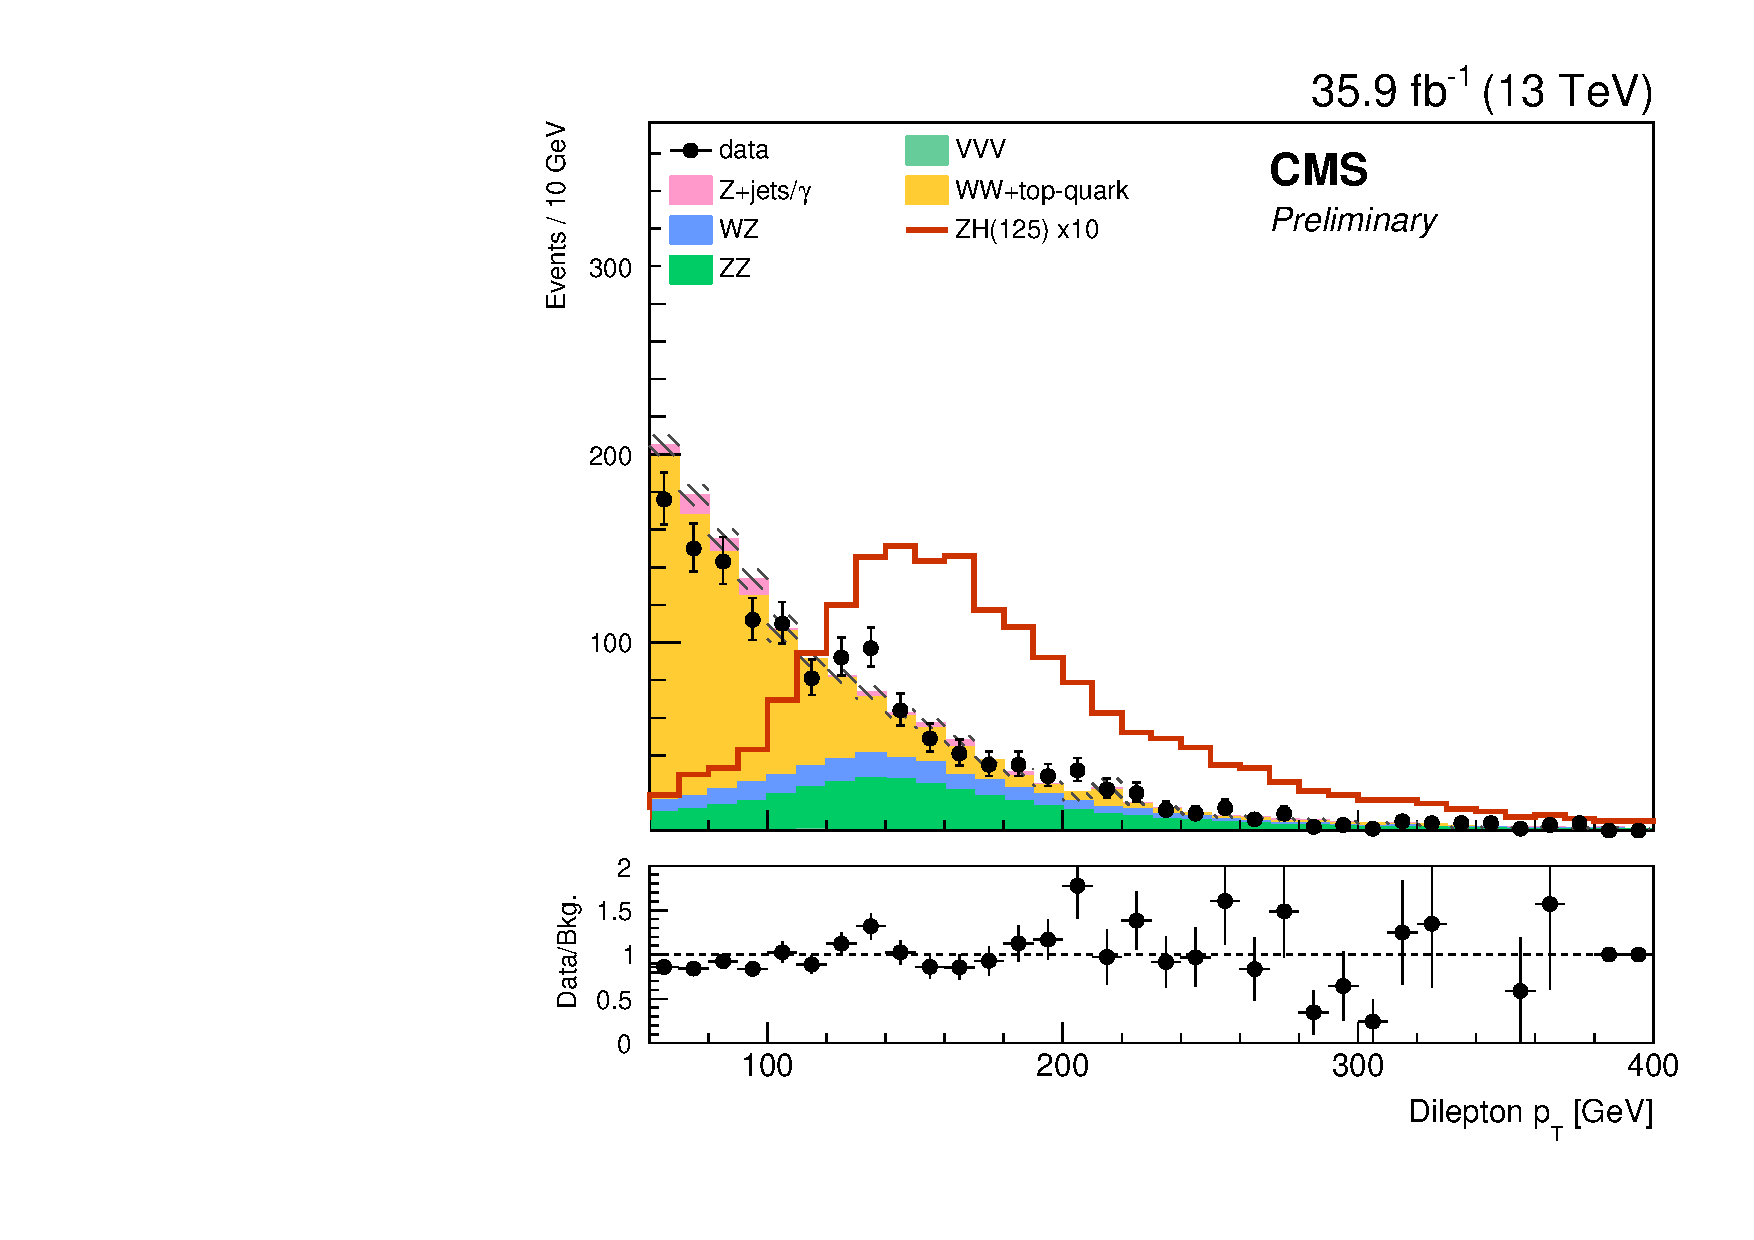
\includegraphics[width=0.48\textwidth]{figures/mva_ptll_nice.pdf}
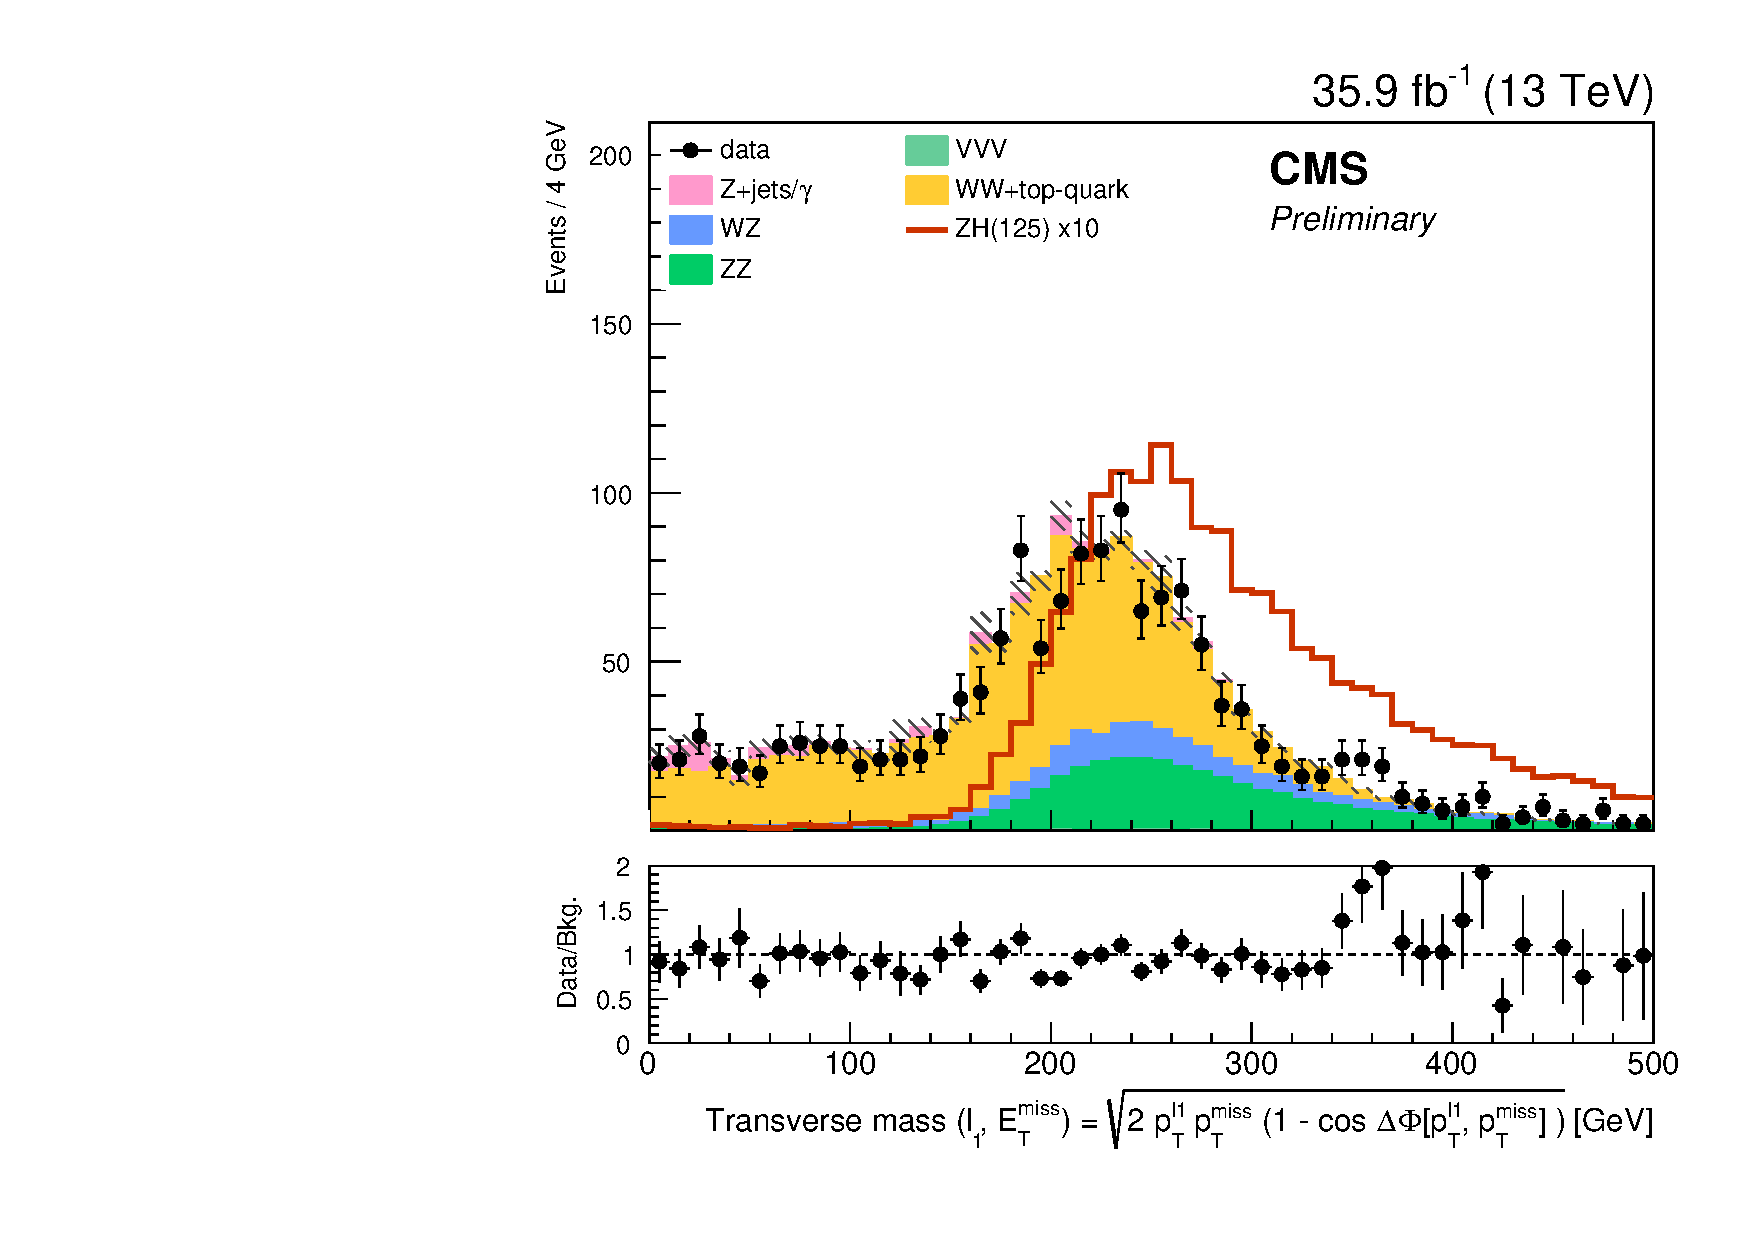
\includegraphics[width=0.48\textwidth]{figures/mva_mTl1MET_nice.pdf}
\caption{Comparison of data and prediction in the BDT input variables after applying the training preselection. Signal strength has been enhanced by a factor of 10.}
\label{fig:bdt_inputvar_histos}
\end{center}
\end{figure}
\begin{figure}[htbp]
\begin{center}
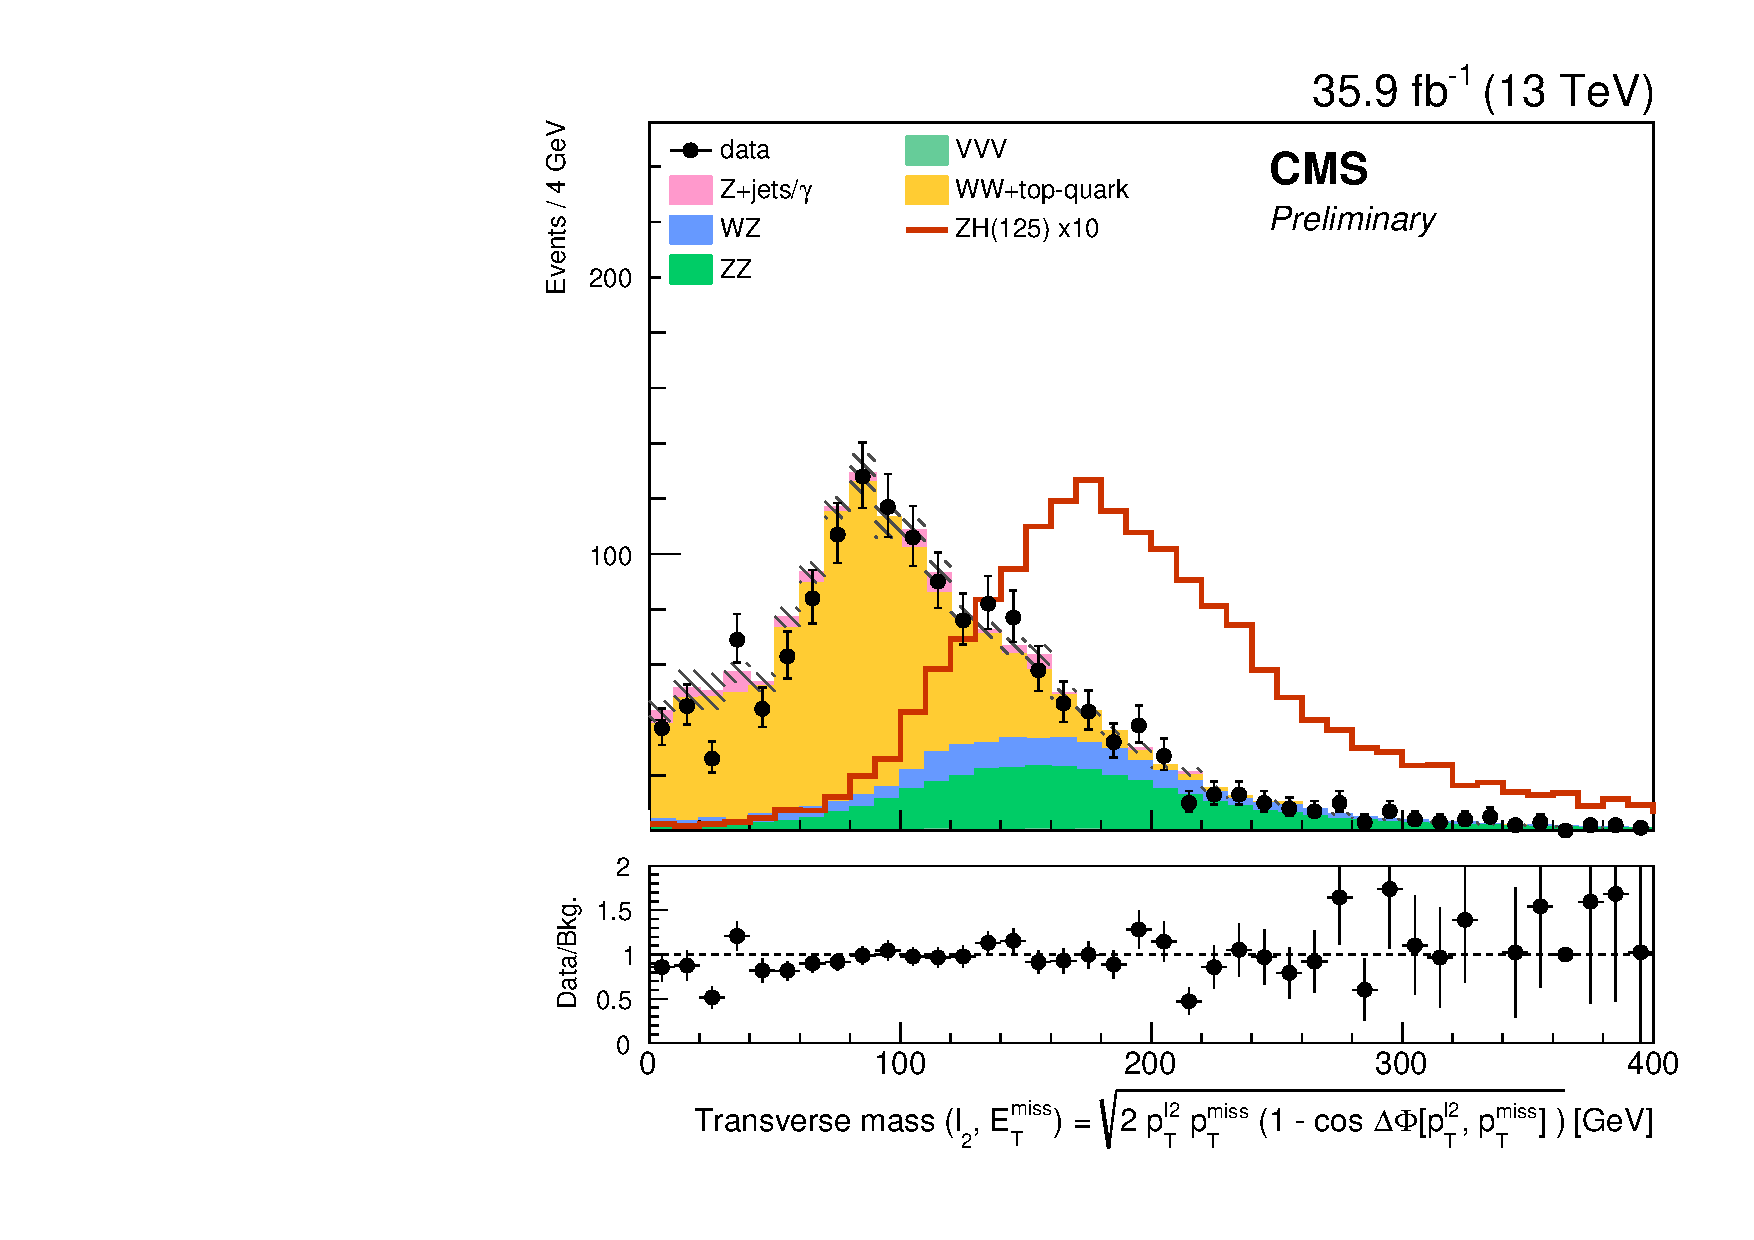
\includegraphics[width=0.48\textwidth]{figures/mva_mTl2MET_nice.pdf}
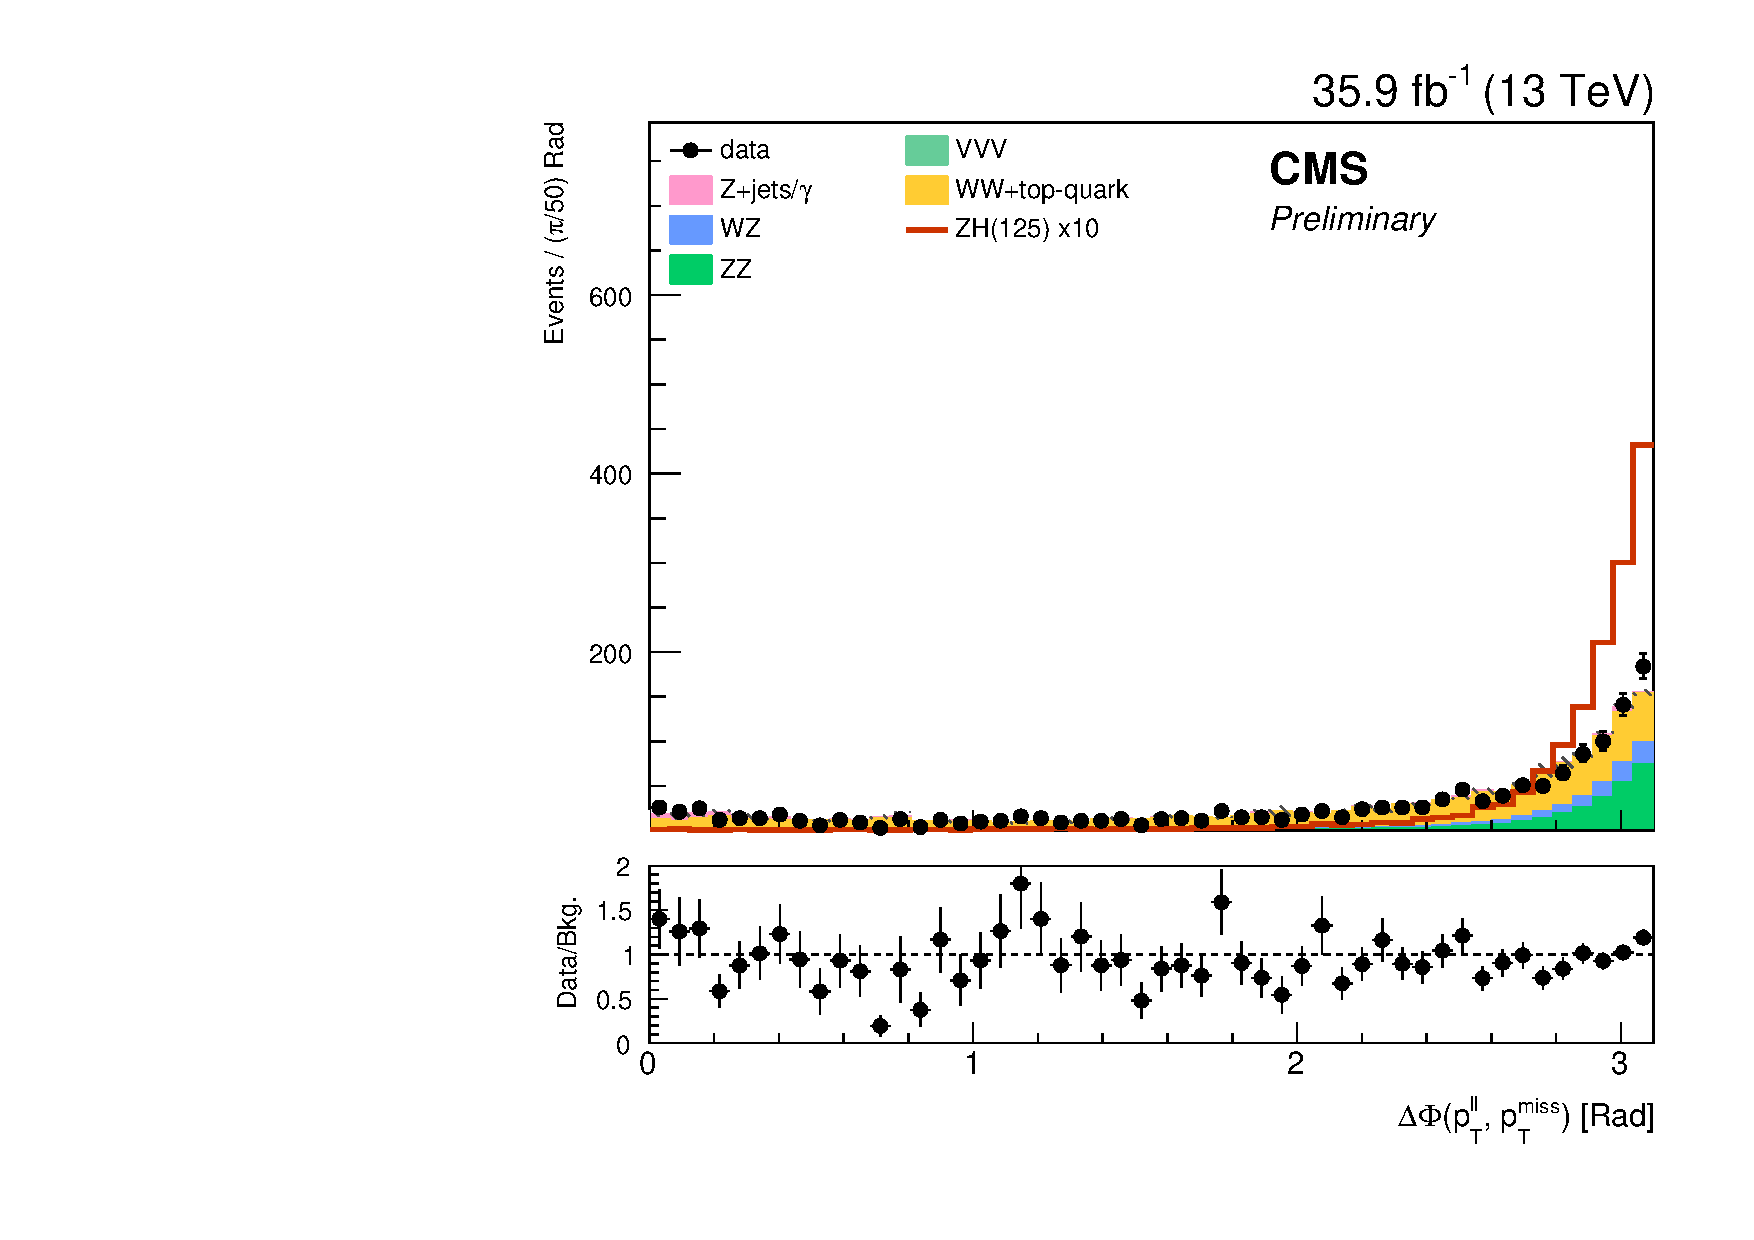
\includegraphics[width=0.48\textwidth]{figures/mva_delphi_ptll_MET_nice.pdf}
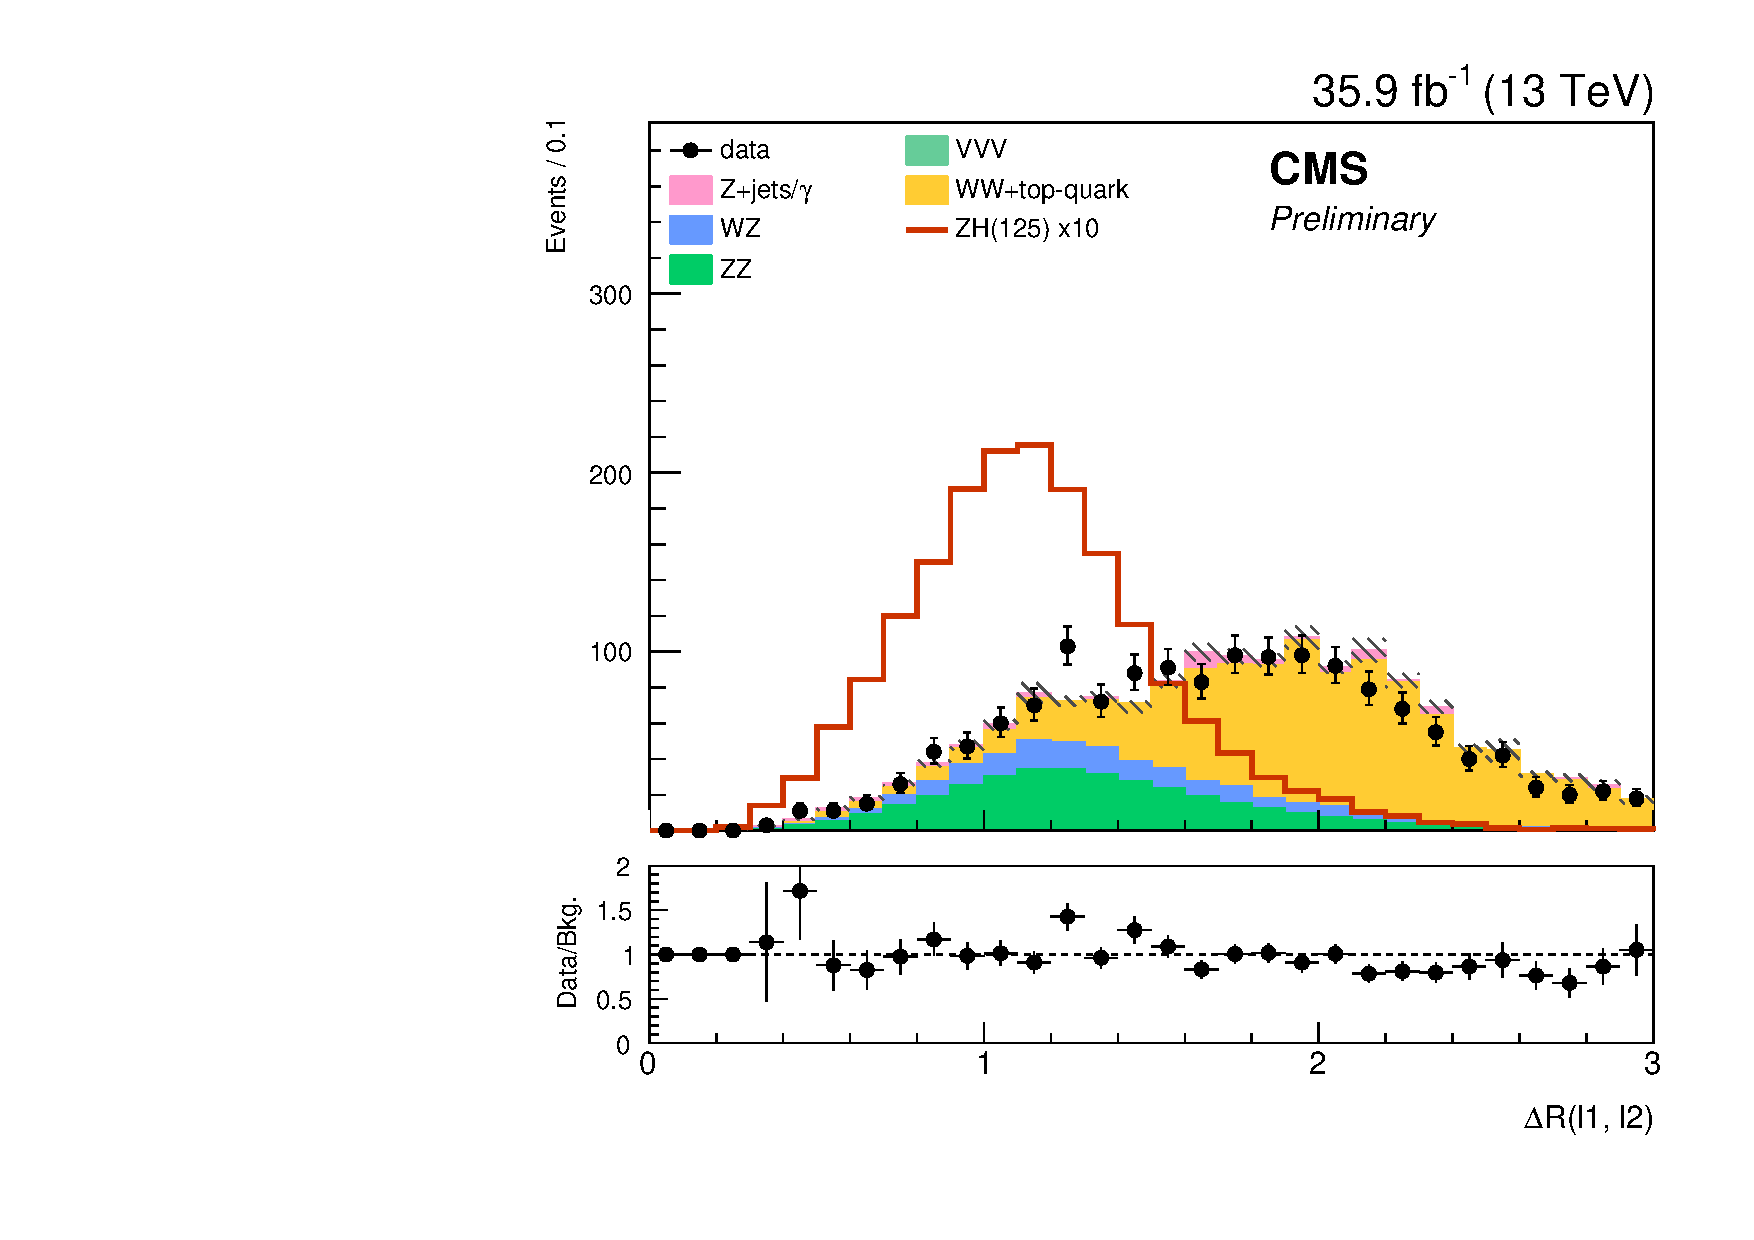
\includegraphics[width=0.48\textwidth]{figures/mva_deltaR_ll_nice.pdf}
%\includegraphics[width=0.48\textwidth]{figures/mva_ptl1mptl2_over_ptll_nice.pdf}
%\includegraphics[width=0.48\textwidth]{figures/mva_cos_theta_star_l1_nice.pdf}
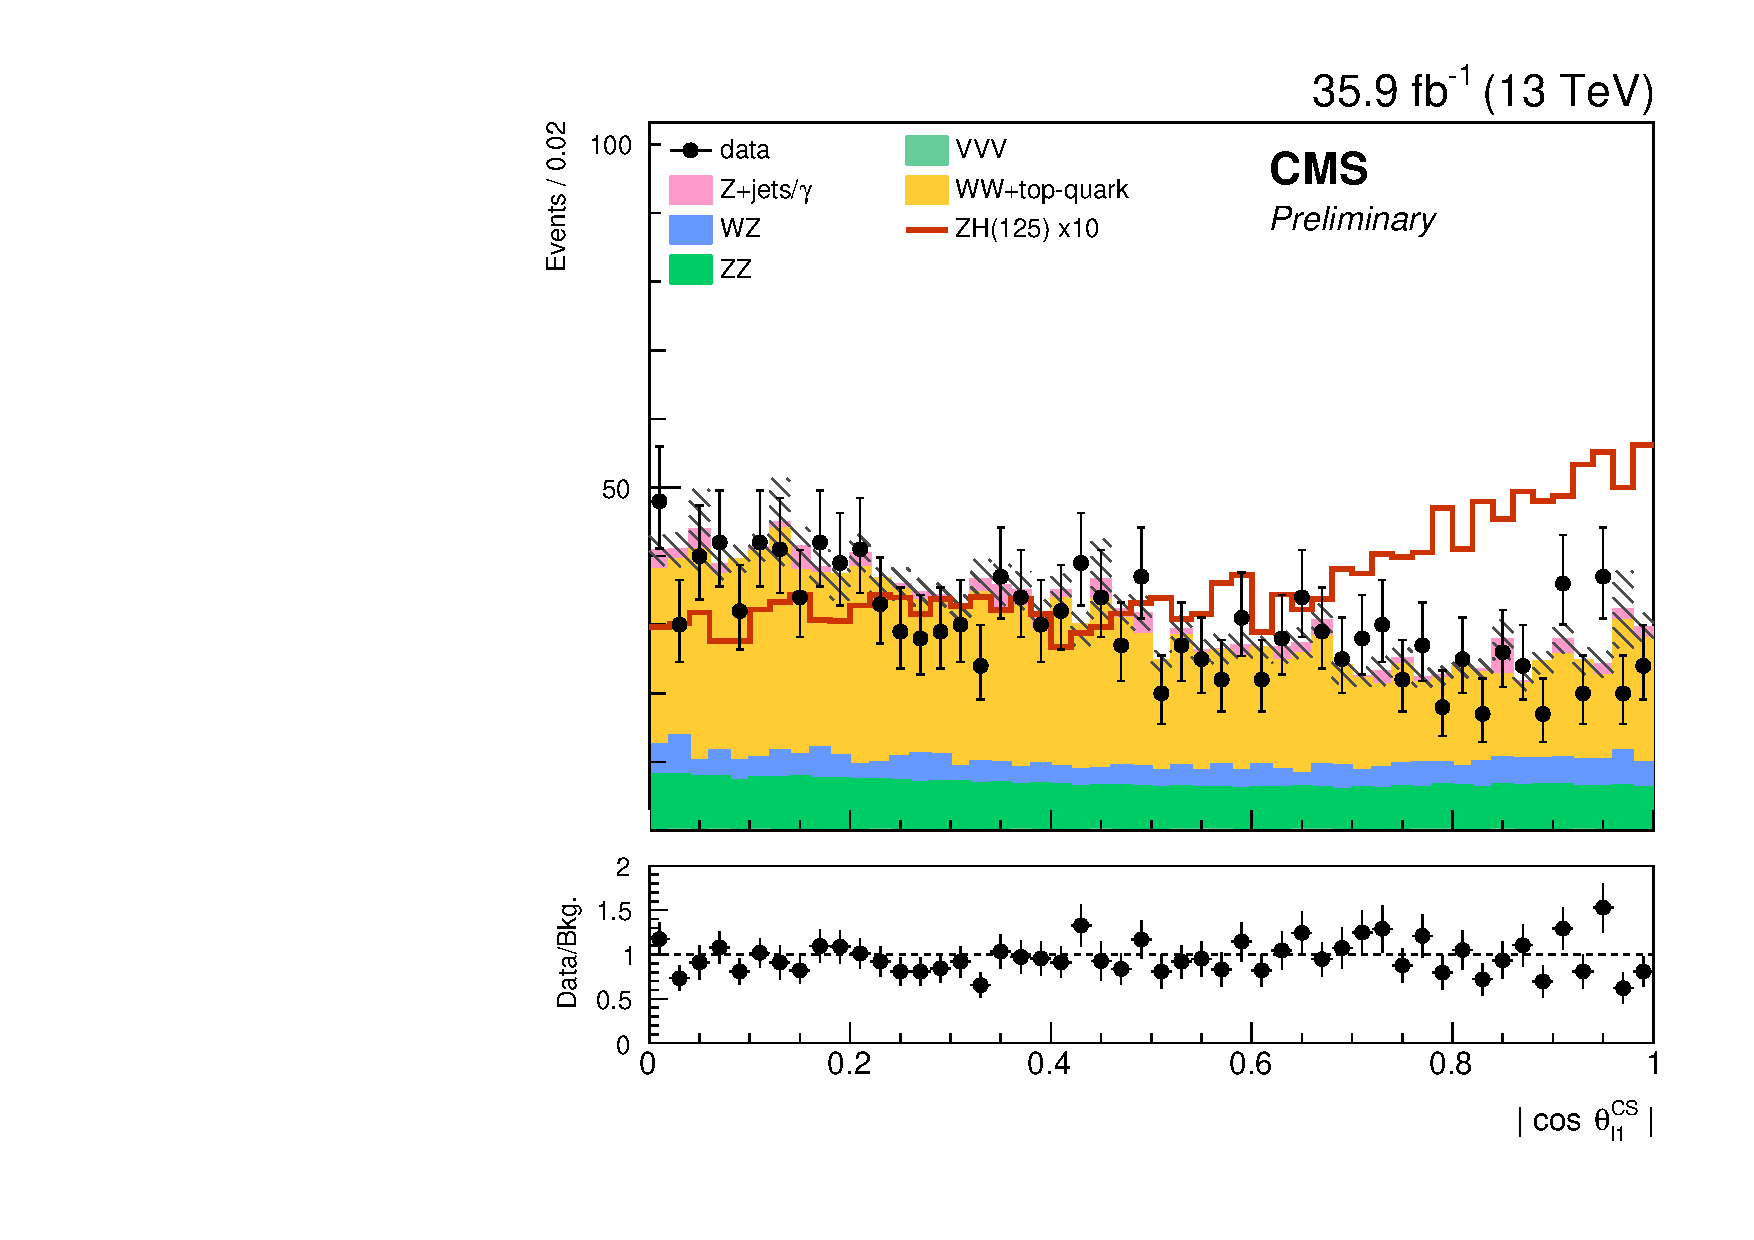
\includegraphics[width=0.48\textwidth]{figures/mva_abs_cos_theta_CS_l1_nice.pdf}
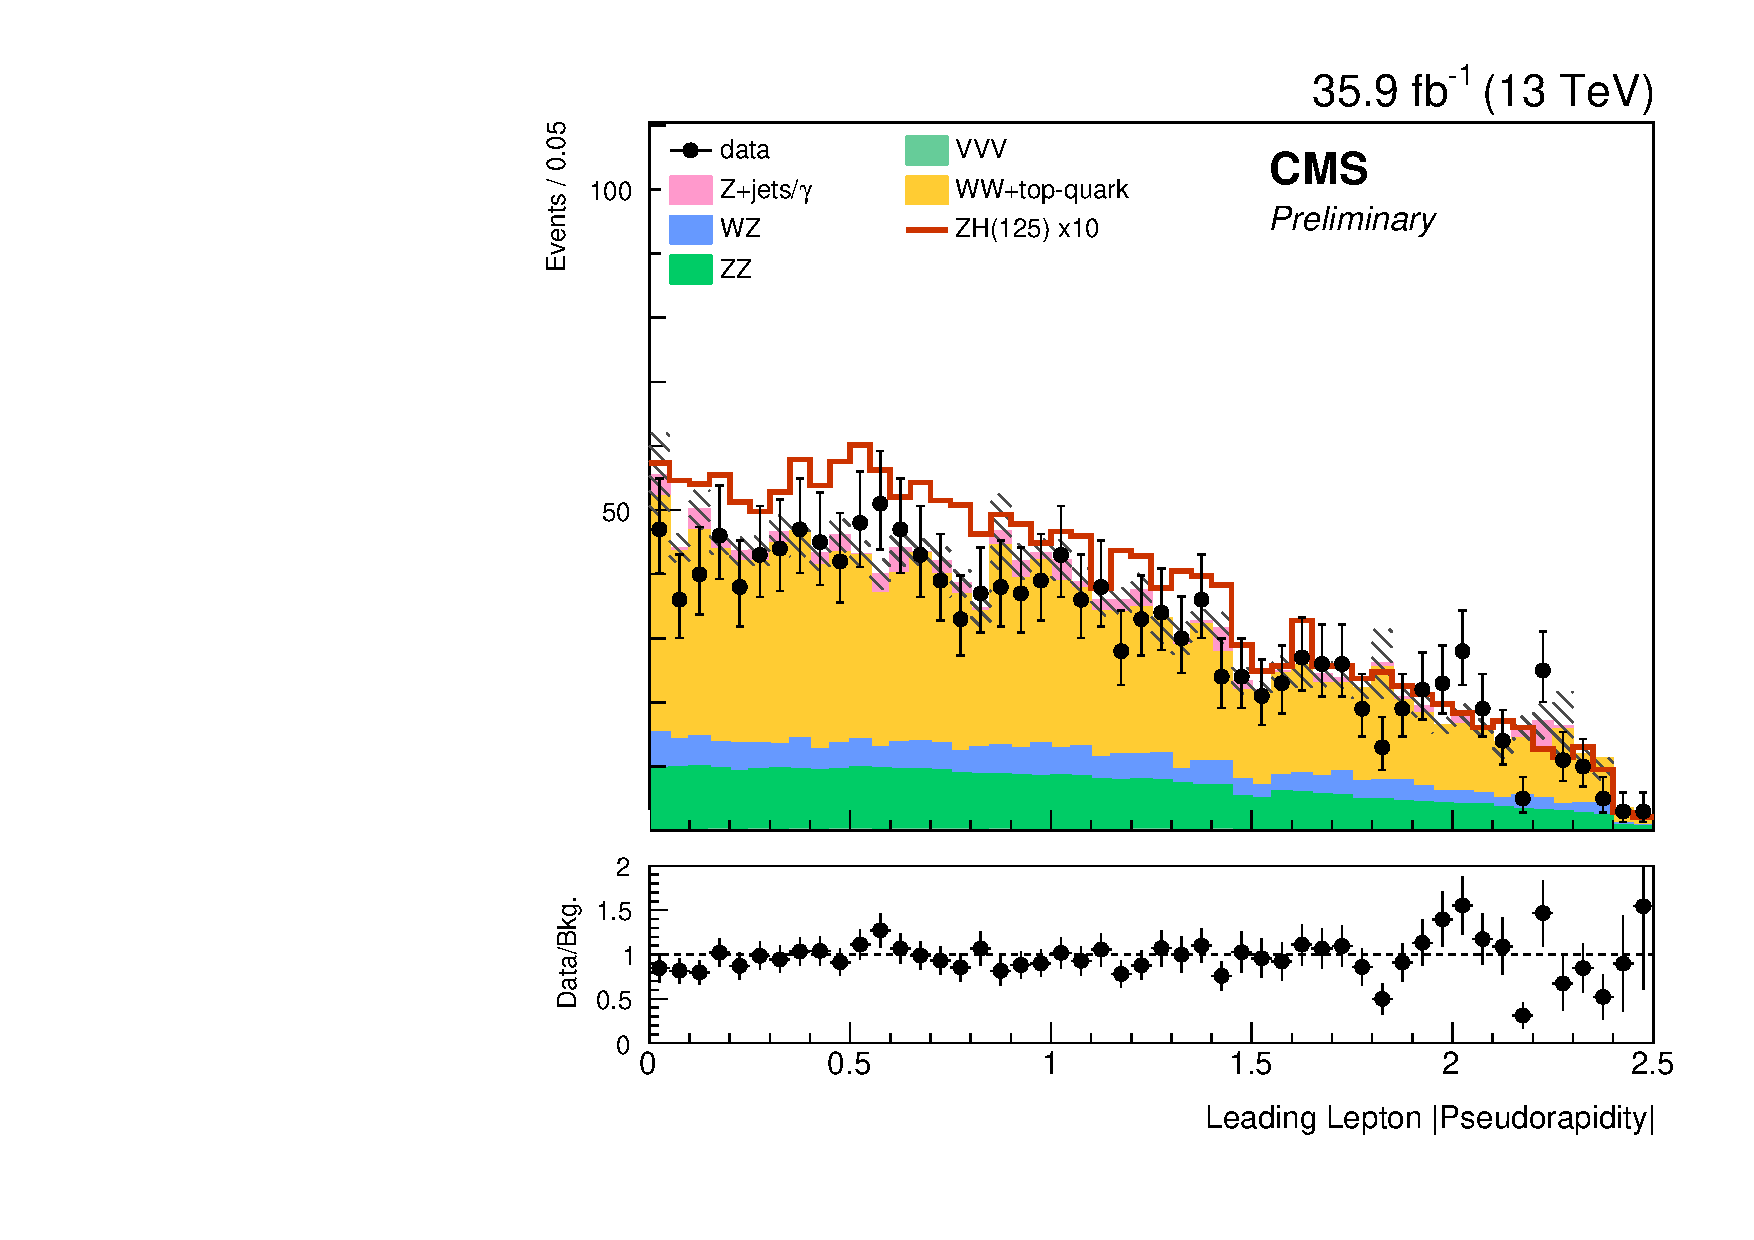
\includegraphics[width=0.48\textwidth]{figures/mva_abs_etal1_nice.pdf}
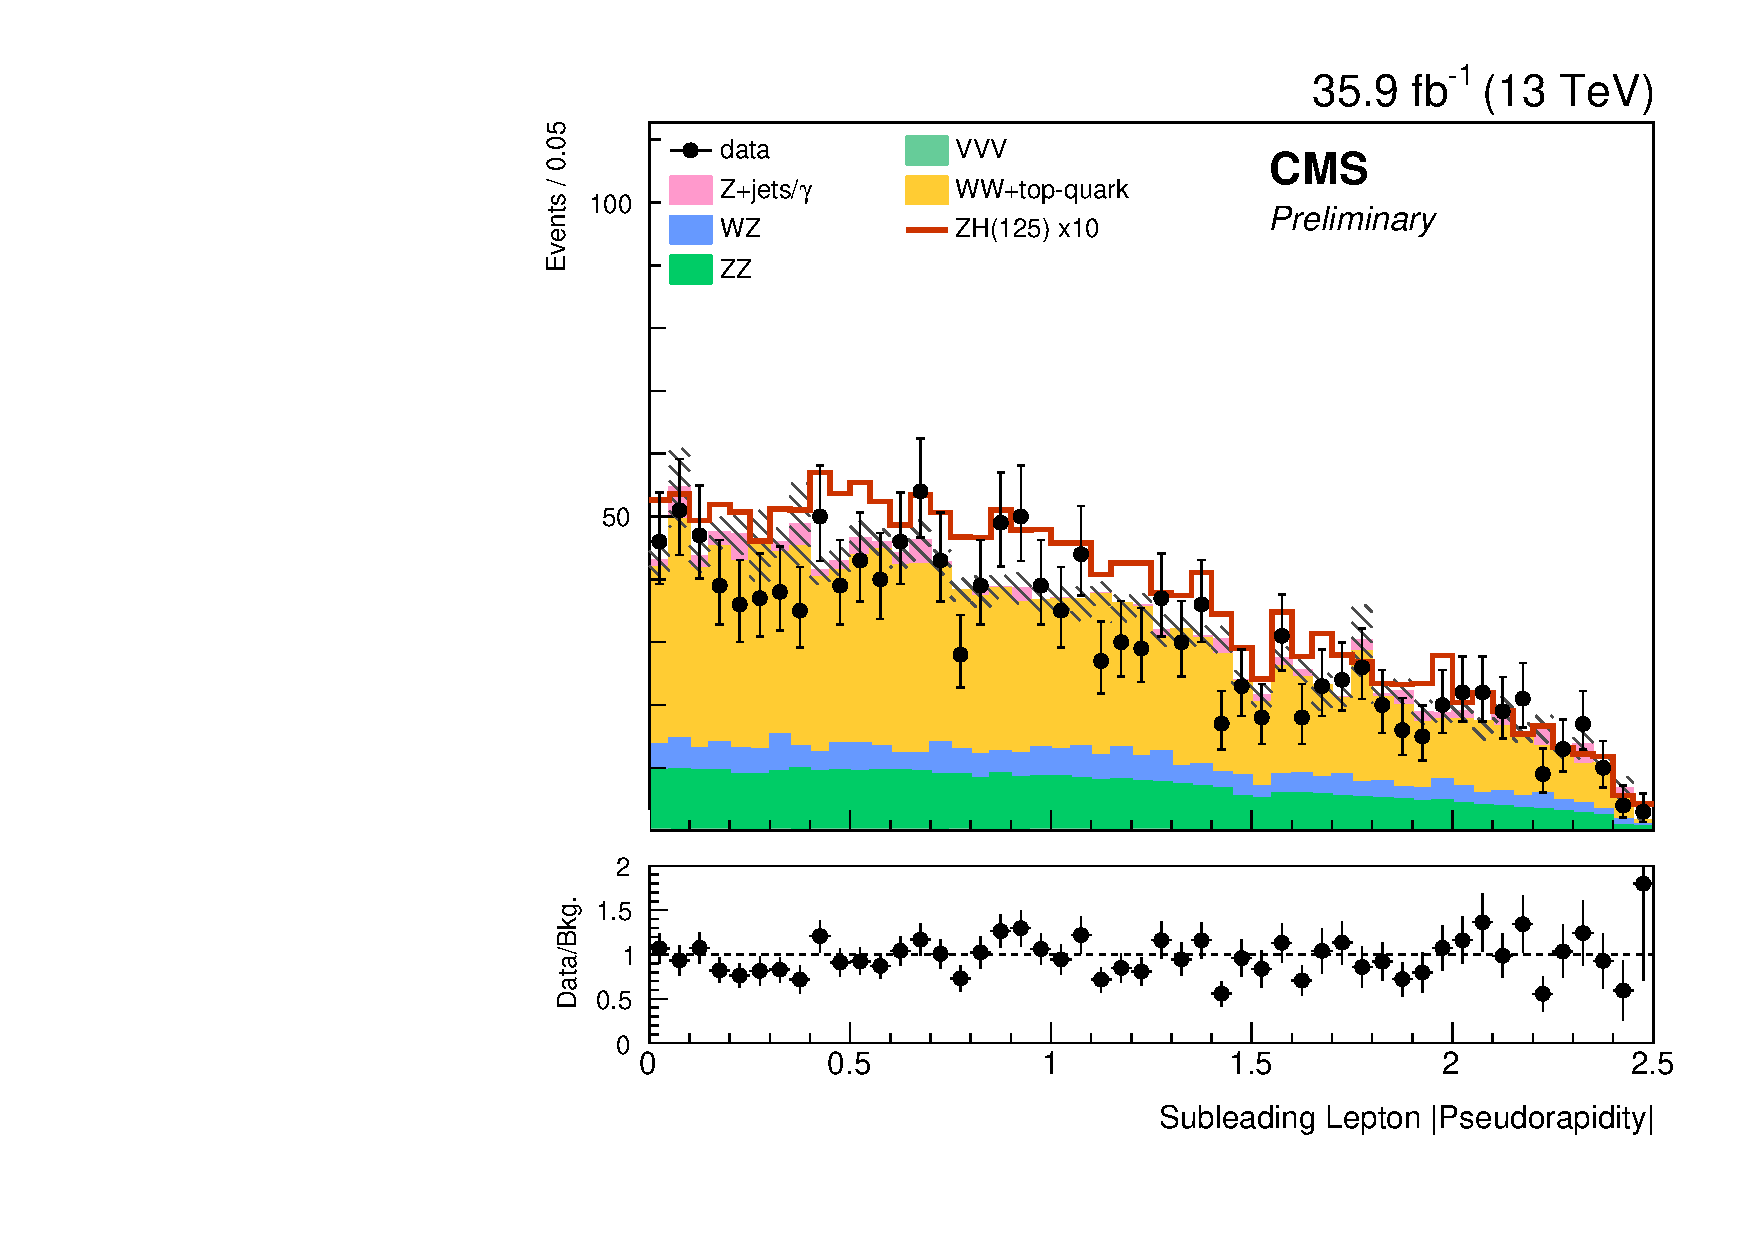
\includegraphics[width=0.48\textwidth]{figures/mva_abs_etal2_nice.pdf}
\caption{(continued, 1) Comparison of data and prediction in the BDT input variables after applying the training preselection. Signal strength has been enhanced by a factor of 10.}
\label{fig:bdt_inputvar_histos2}
\end{center}
\end{figure}


\section{Mapping the experimental uncertainties}
\label{sec:bdt_toys}
In order to perform a shape analysis in the classifier BDT spectrum, the effect of various nuisance parameters must be propagated to the BDT shape.
It is not sufficient to simply evaluate different shapes at the extremities of the nuisance variations, because a BDT is not a conformal map.
Therefore, we used a toy method to sample the distributions of the relevant nuisance parameters and found the resulting distributions in BDT value.
The nuisances considered to be relevant are the uncertainty of the lepton momentum scale (see Section~\ref{subsec:lepres}) and the uncertainty of missing energy due to the jet energy scale (JES).

The number of random toys used for the uncertainty propagation was 50 due to the high computing cost of many classifier evaluations. 
The lepton scale variations were sampled from a normal distribution with standard deviation of 0.01.
The \met variations were sampled from a normal distribution with standard deviation of 1, then multiplied by the relative size of the jet energy scale effect (this quantity varies per event).
Variations in the lepton scale affected the missing energy which was adjusted; variations in the missing energy affected many of the other variables, which were subsequently adjusted. 

After performing this procedure for all simulated events, we take the uncertainty bands from the non-normal toy distributions as the distance between the 15.9\% and 84.1\% quantiles.
These are the so-called $\pm1\sigma$ quantiles of a normal distribution.

Figures~\ref{fig:bdt_toy_envelopes_electron},~\ref{fig:bdt_toy_envelopes_muon}, and~\ref{fig:bdt_toy_envelopes_MET} show 2D maps of the nuisance variations with the BDT value on the horizontal axis and the relative variation from the nominal BDT bin yield on the vertical axis.
Figures~\ref{fig:bdt_electron_scale},~\ref{fig:bdt_muon_scale}, and~\ref{fig:bdt_MET_scale} show the resulting uncertainty shapes that enter the likelihood fit, for the electron scale, muon scale, and MET scale nuisances respectively. 
In most combinations of background process and nuisance parameter, the propagated uncertainty is irrelevant compared to the statistical uncertainty from the number of simulated events.

We do not propagate this uncertainty for the non-resonant backgrounds or the Drell-Yan process, 
since they are not highly signal-like and the other extrapolation uncertainties are sufficiently conservative.
Furthermore, when performing the likelihood fit to determine the exclusion limits, 
we ignore these propagated uncertainties in the ratio of the diboson control regions, 
and fully correlate them across the shape bins in the signal region. 

\begin{figure}[htbp]
\begin{center}
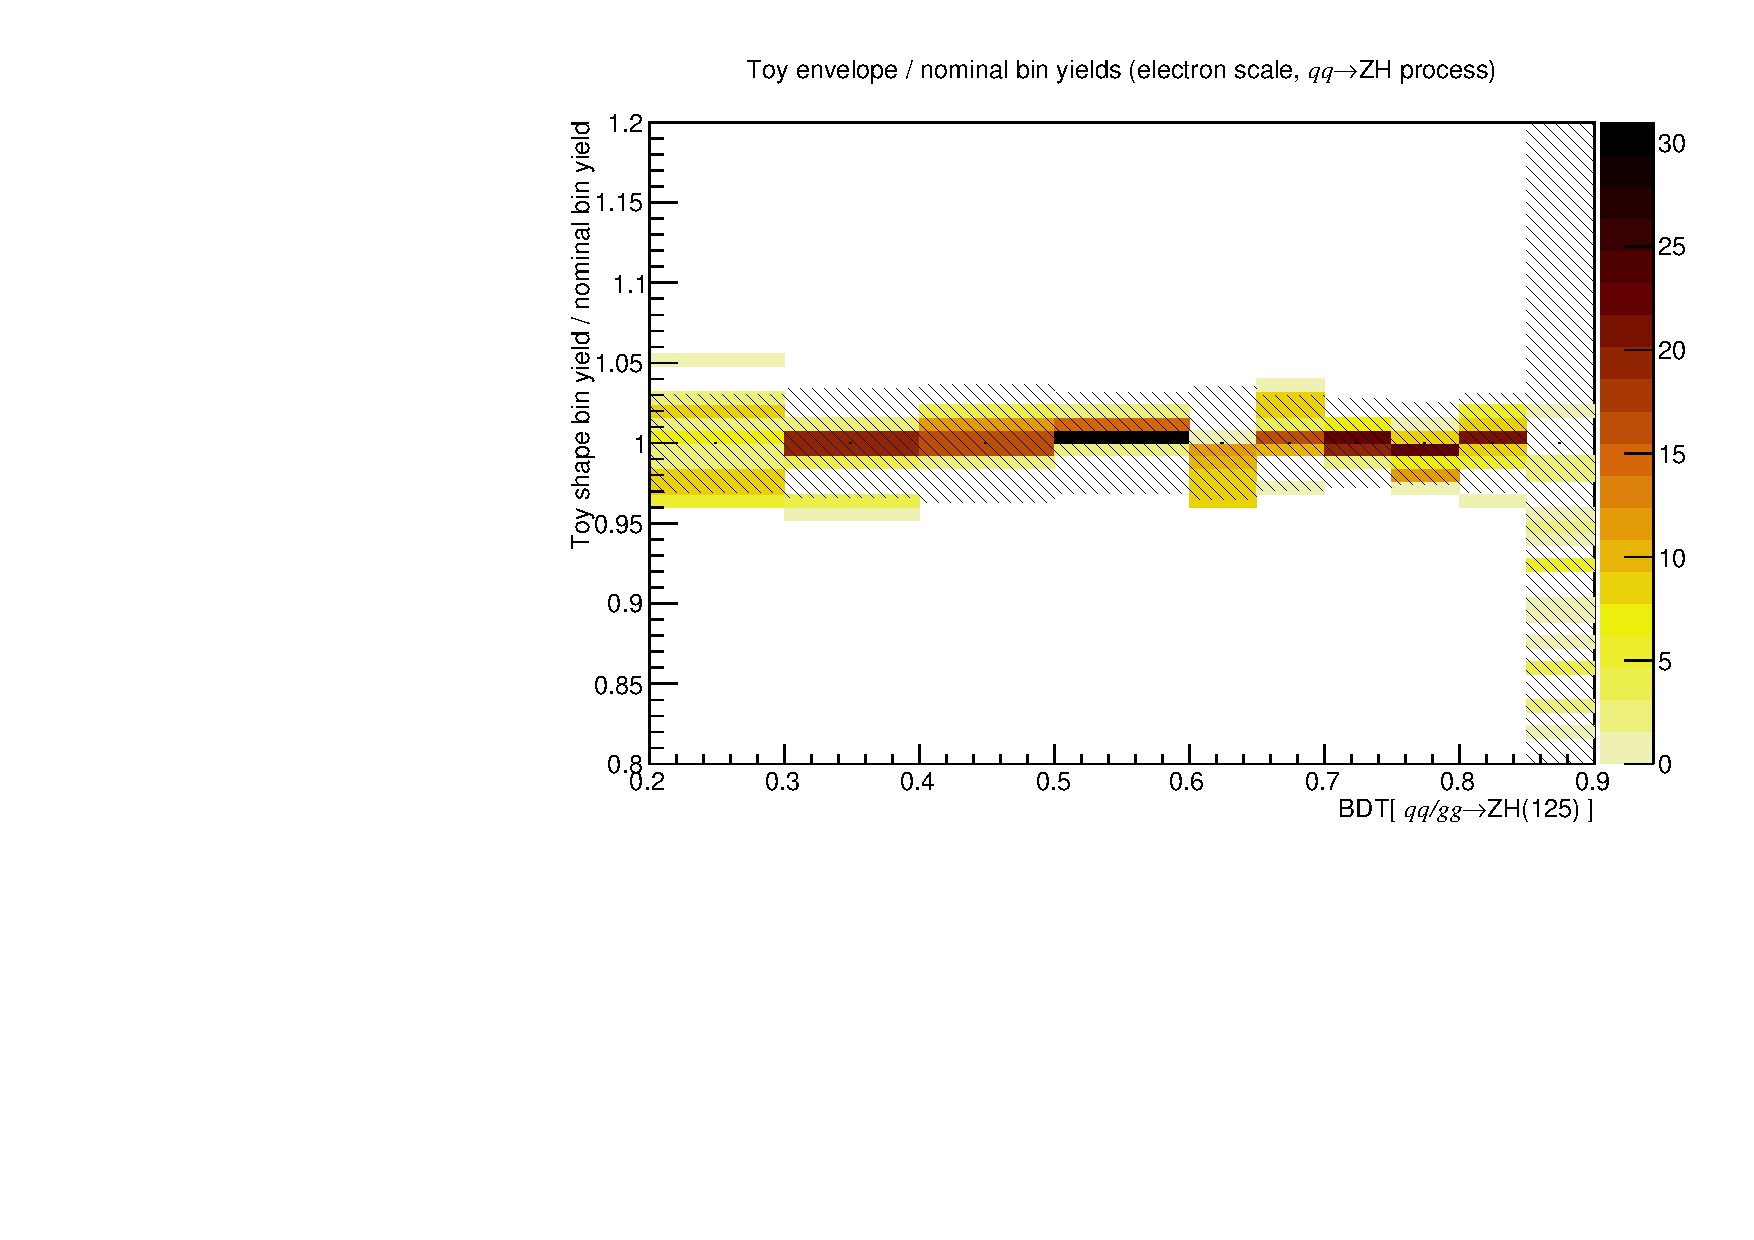
\includegraphics[width=0.48\textwidth]{figures/syst_BDT_ZH_hinv_sm_toyenvelope_electron.pdf}
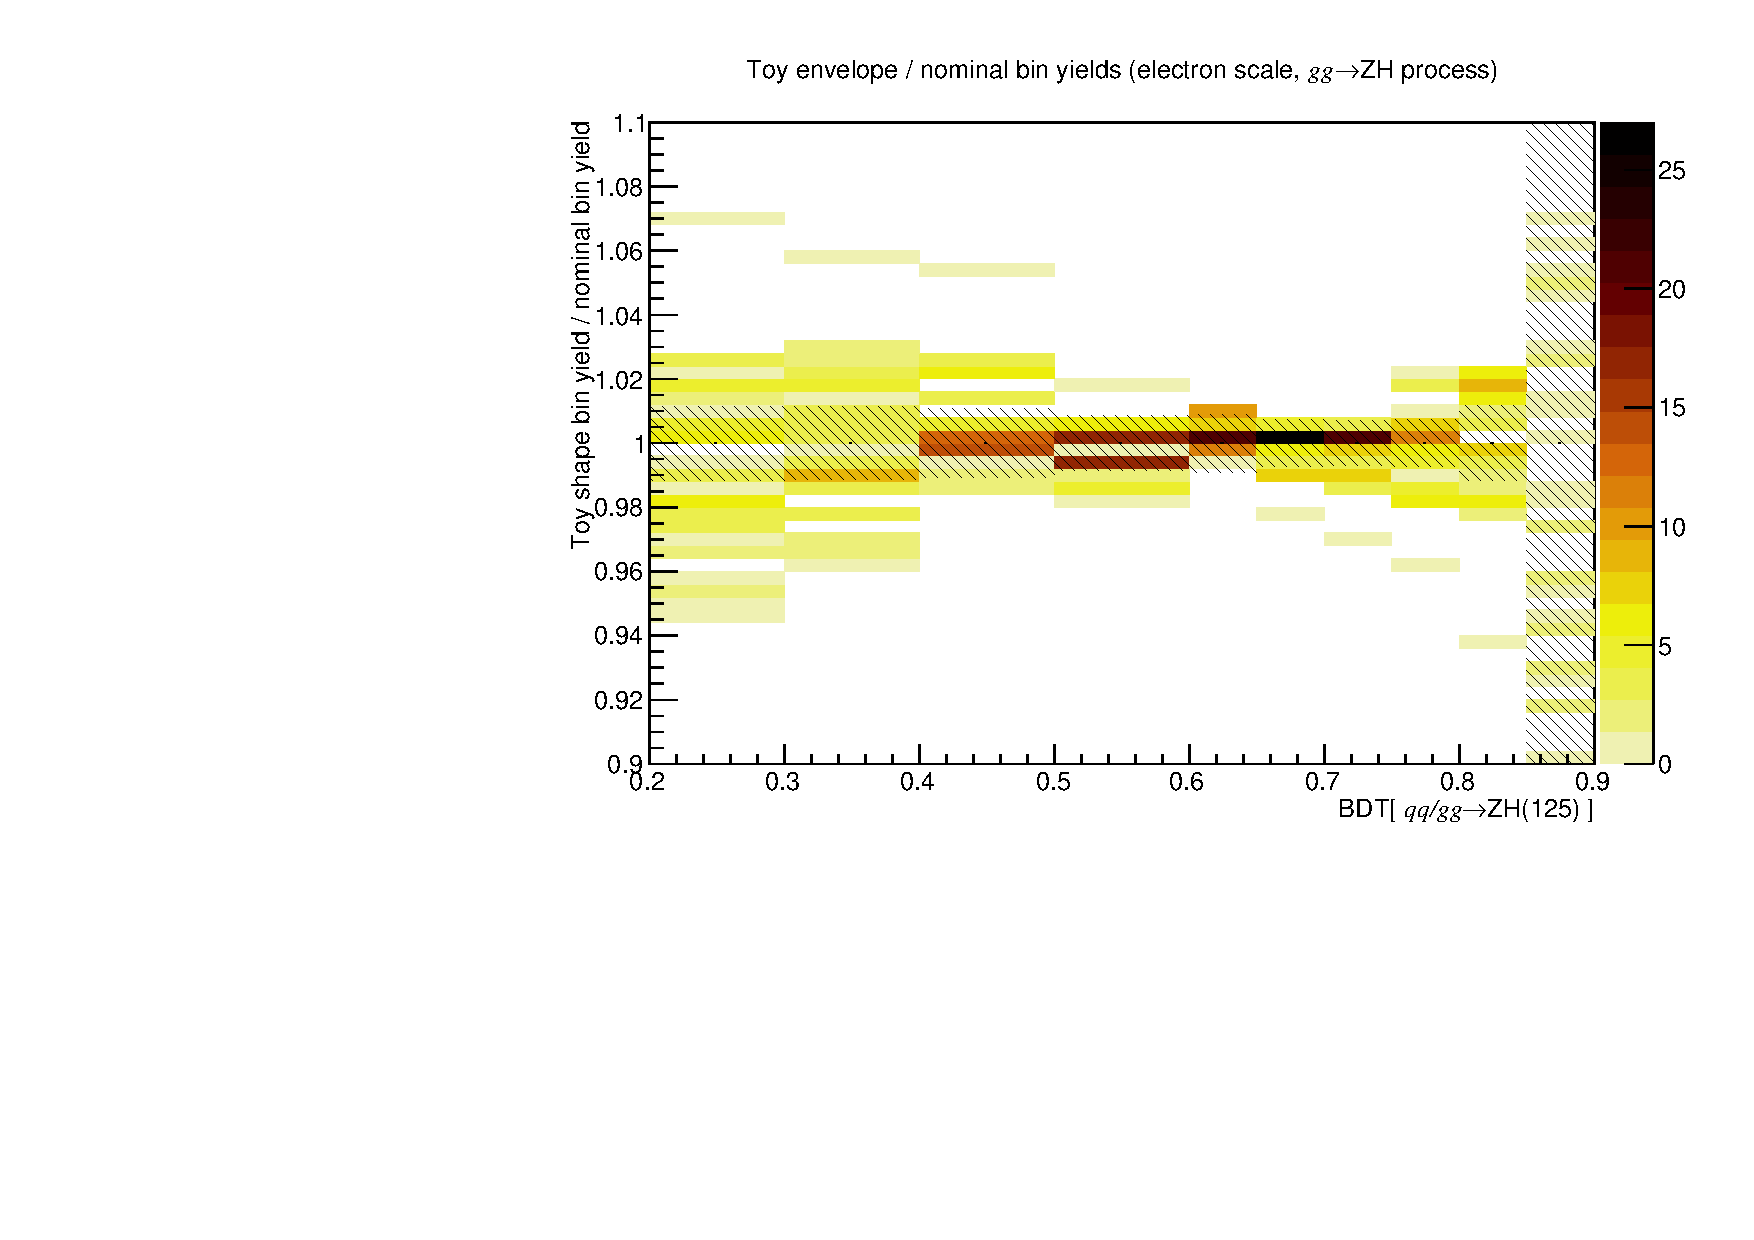
\includegraphics[width=0.48\textwidth]{figures/syst_BDT_ggZH_hinv_toyenvelope_electron.pdf}
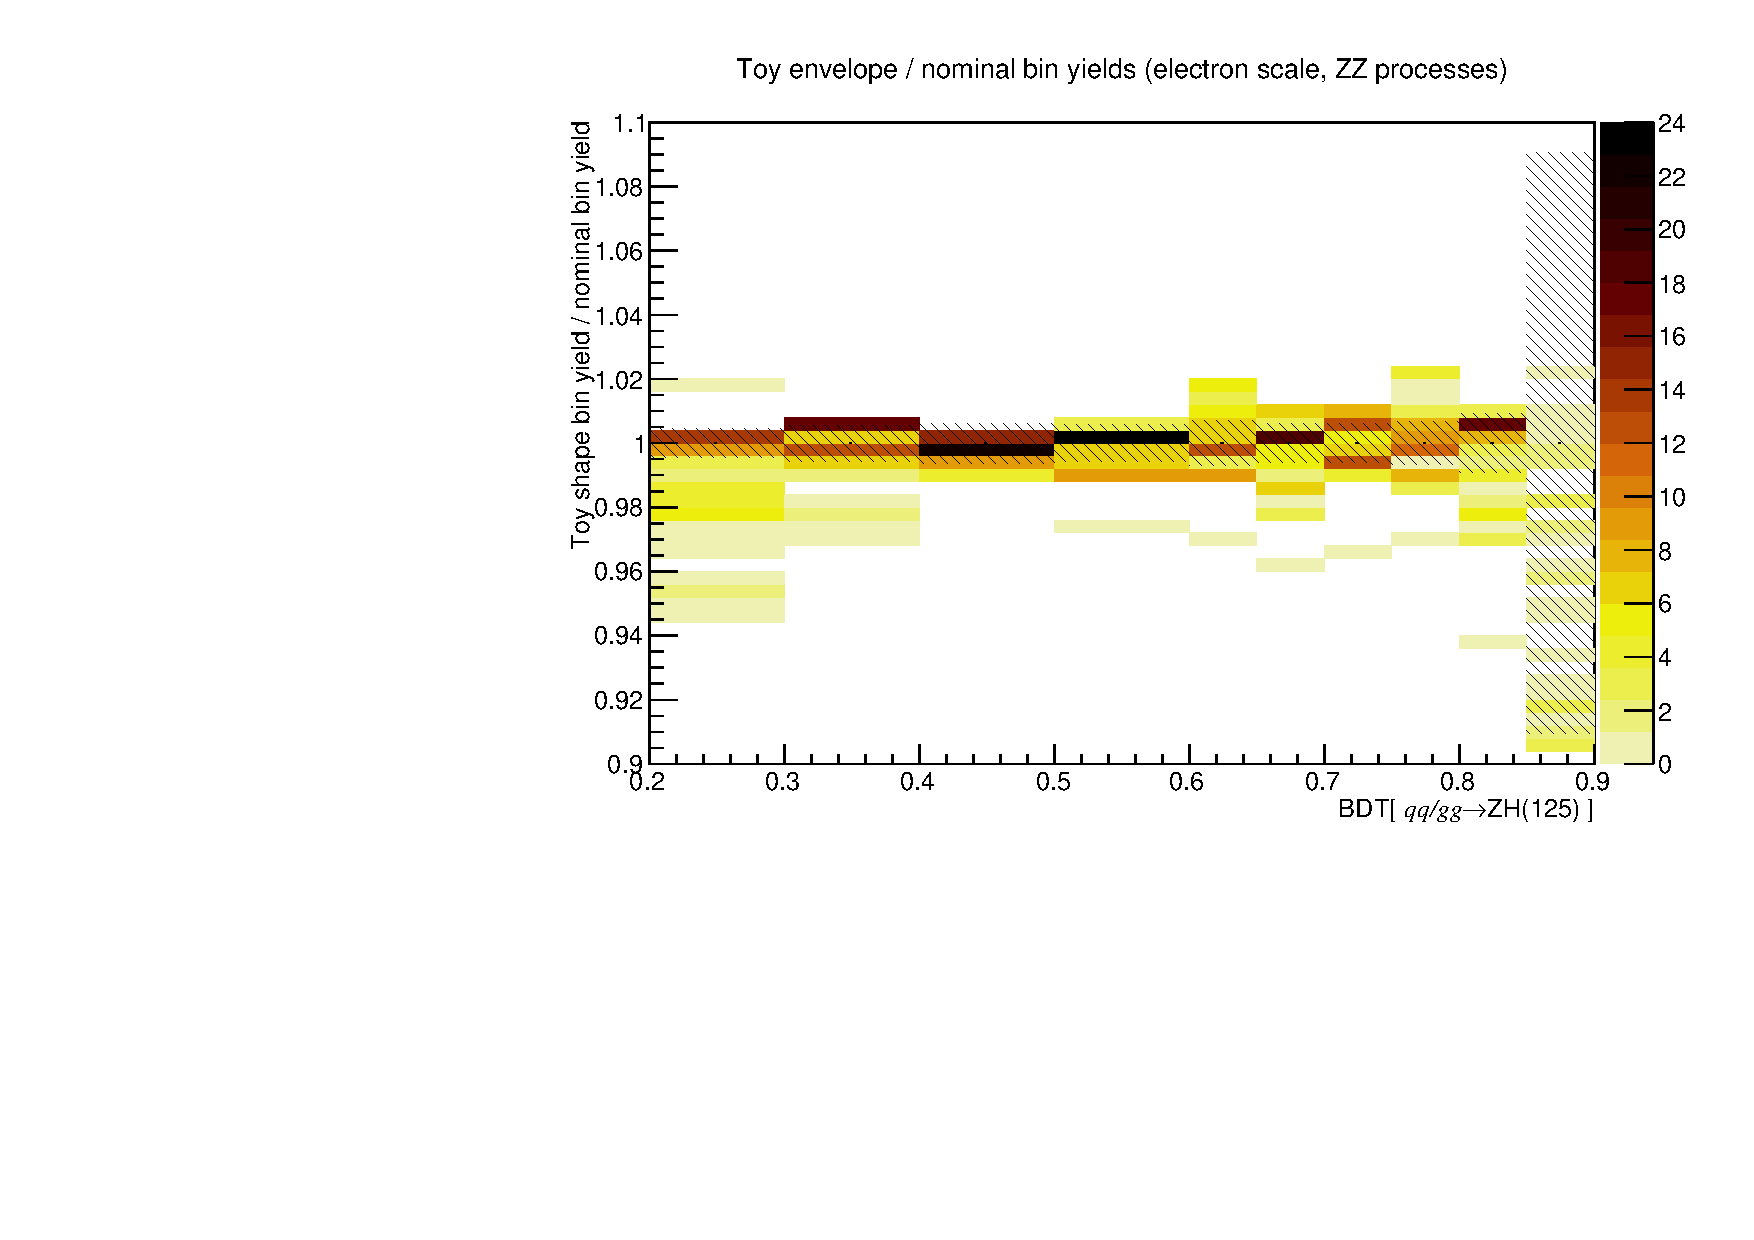
\includegraphics[width=0.48\textwidth]{figures/syst_BDT_ZZ_toyenvelope_electron.pdf}
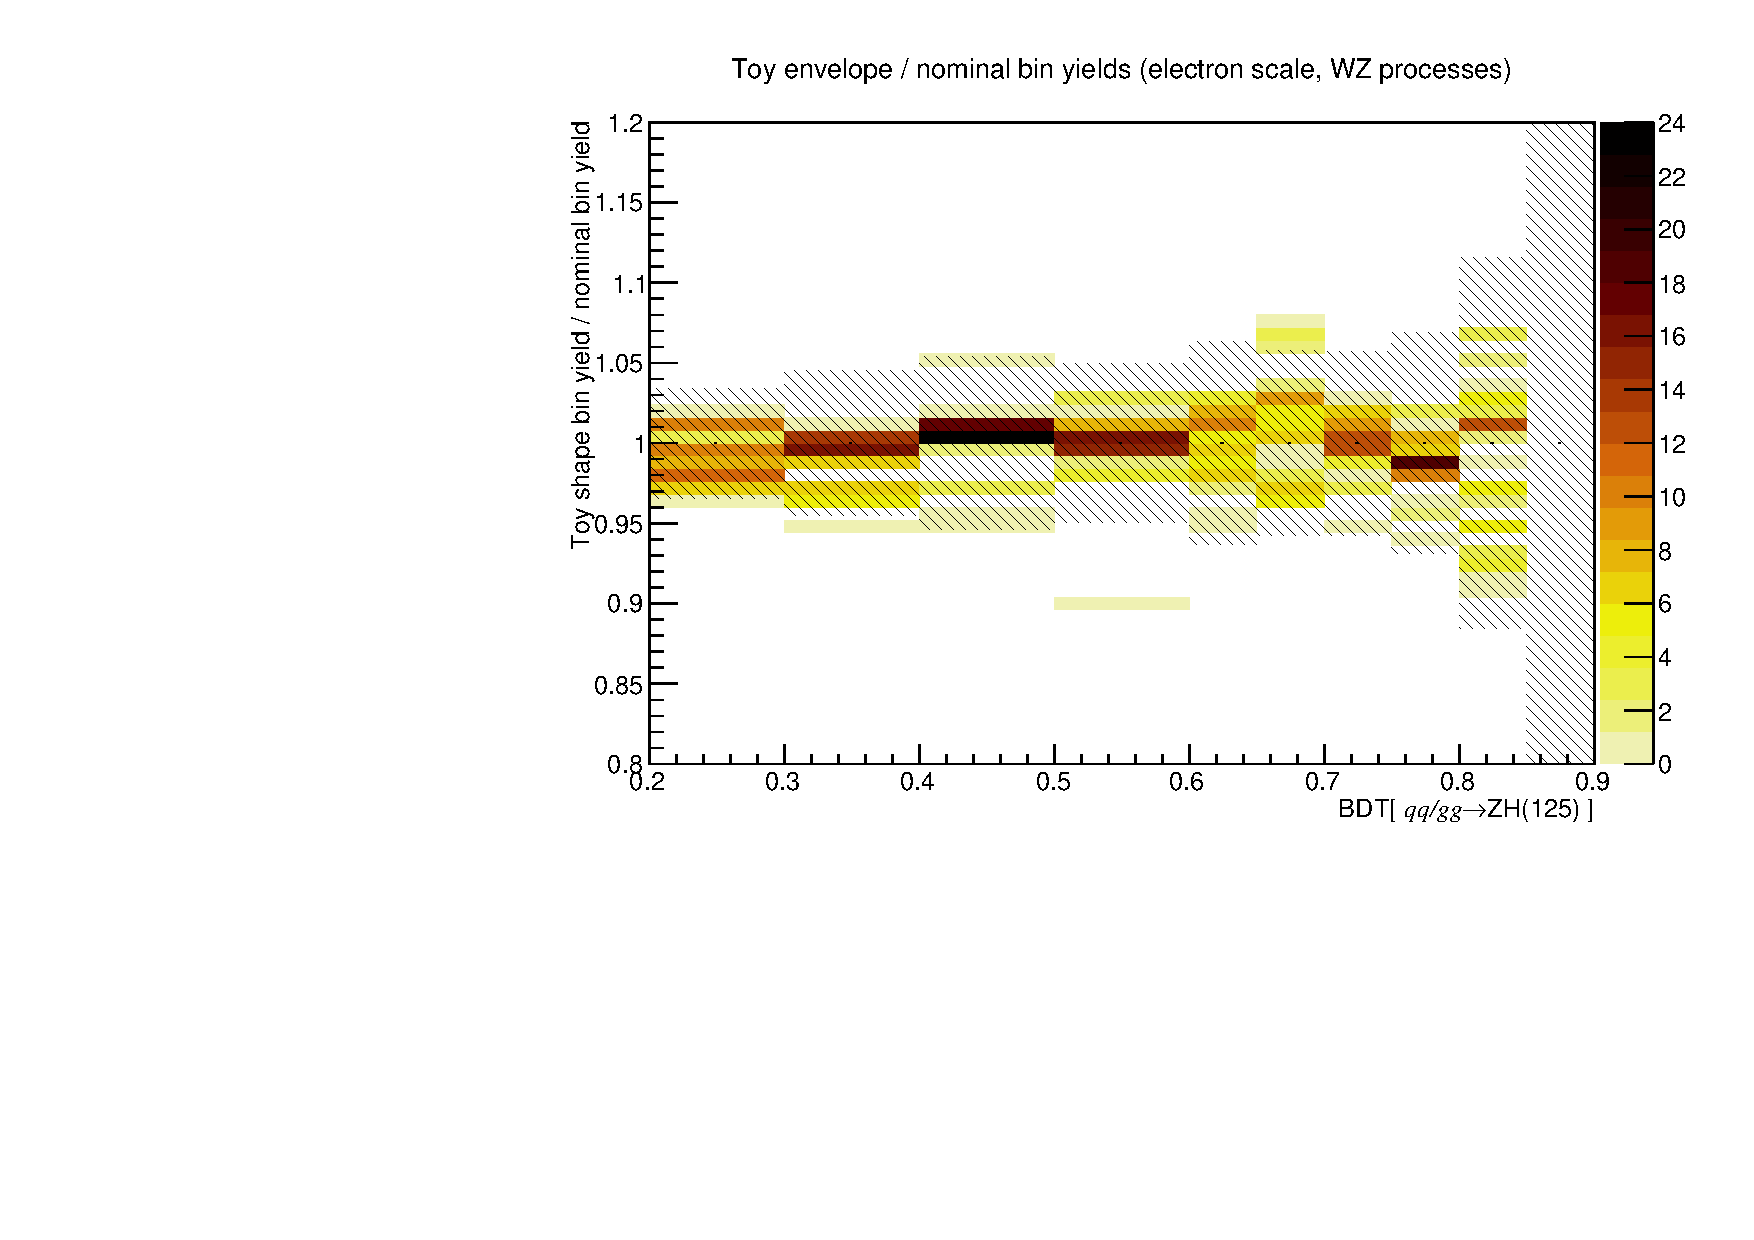
\includegraphics[width=0.48\textwidth]{figures/syst_BDT_WZ_toyenvelope_electron.pdf}
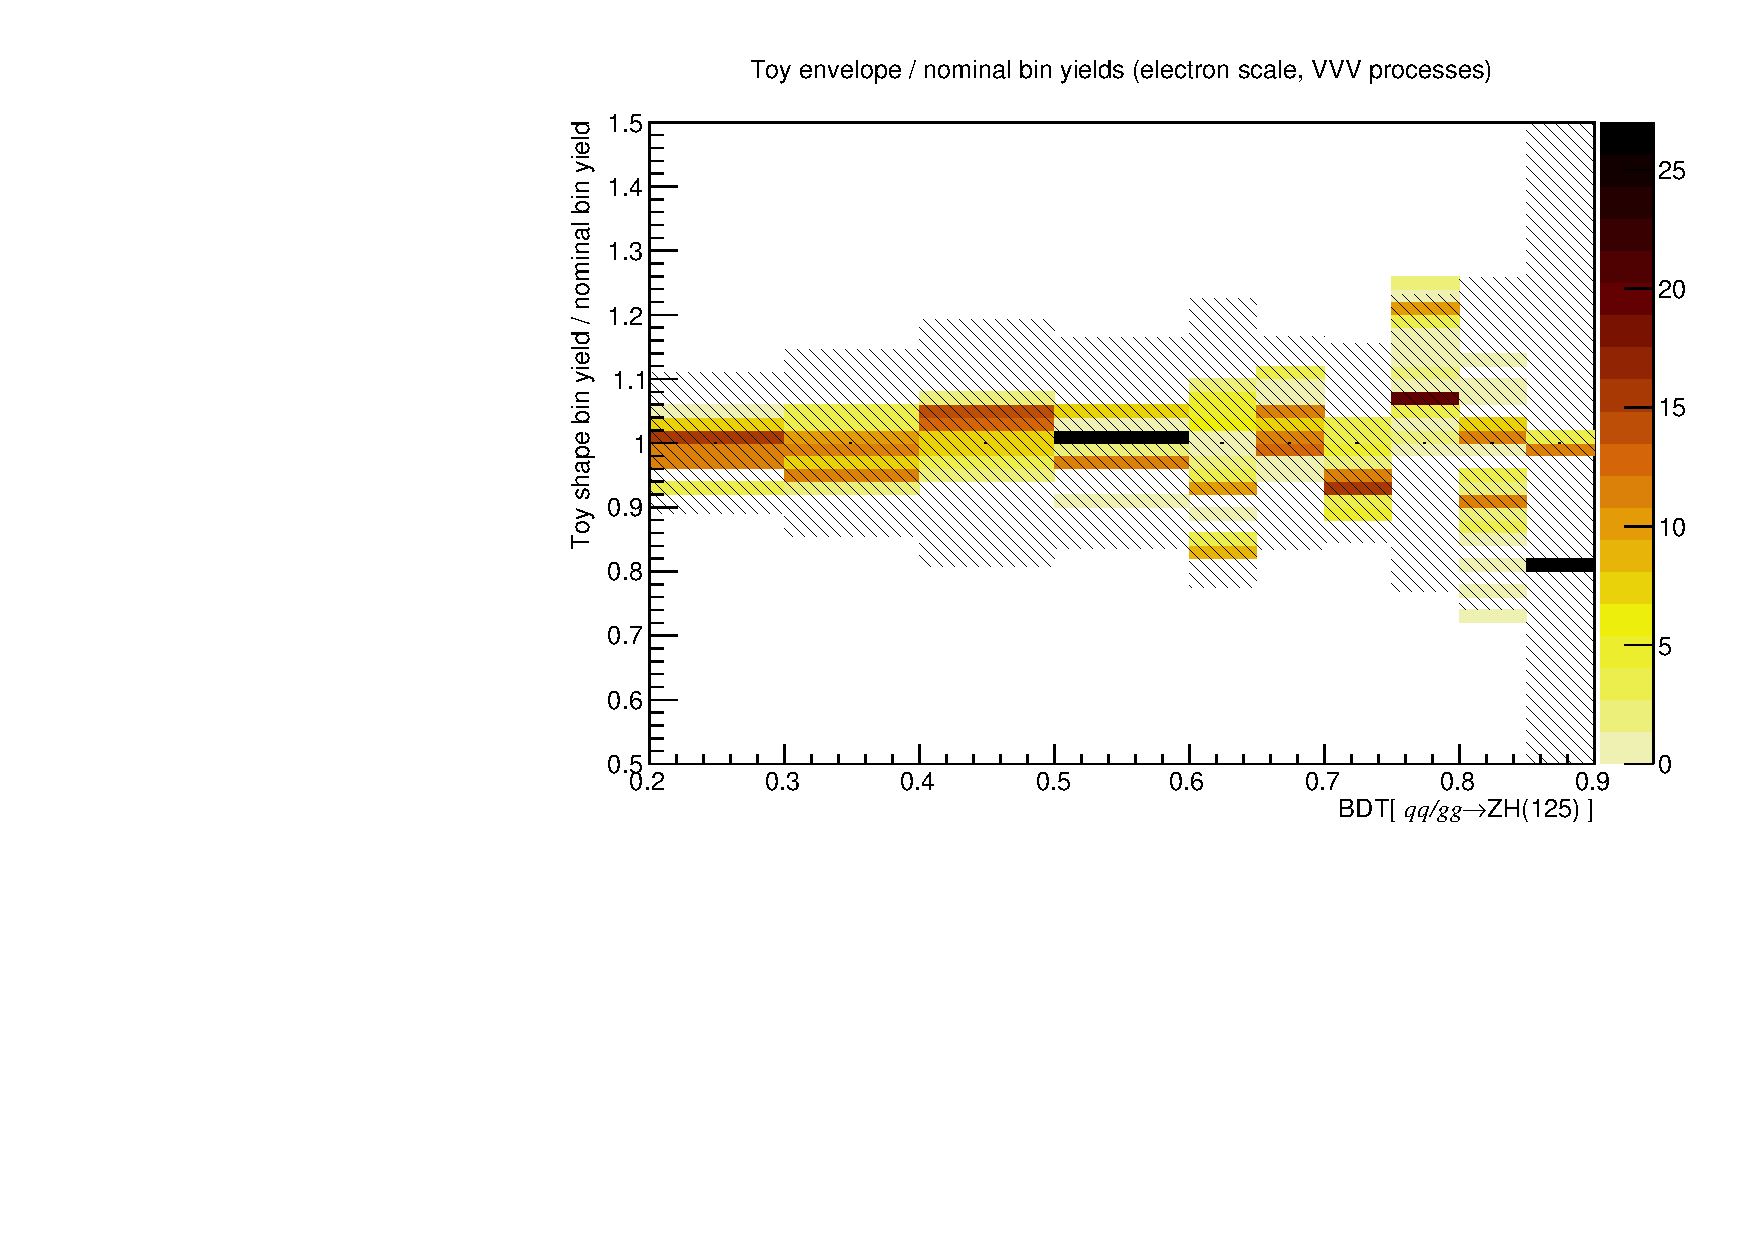
\includegraphics[width=0.48\textwidth]{figures/syst_BDT_VVV_toyenvelope_electron.pdf}
\caption{2D maps of the relative toy variations from the nominal BDT shape versus the BDT value, for the electron scale. The hashed bands represent statistical uncertainty on the simulated events.}
\label{fig:bdt_toy_envelopes_electron}
\end{center}
\end{figure}

\begin{figure}[htbp]
\begin{center}
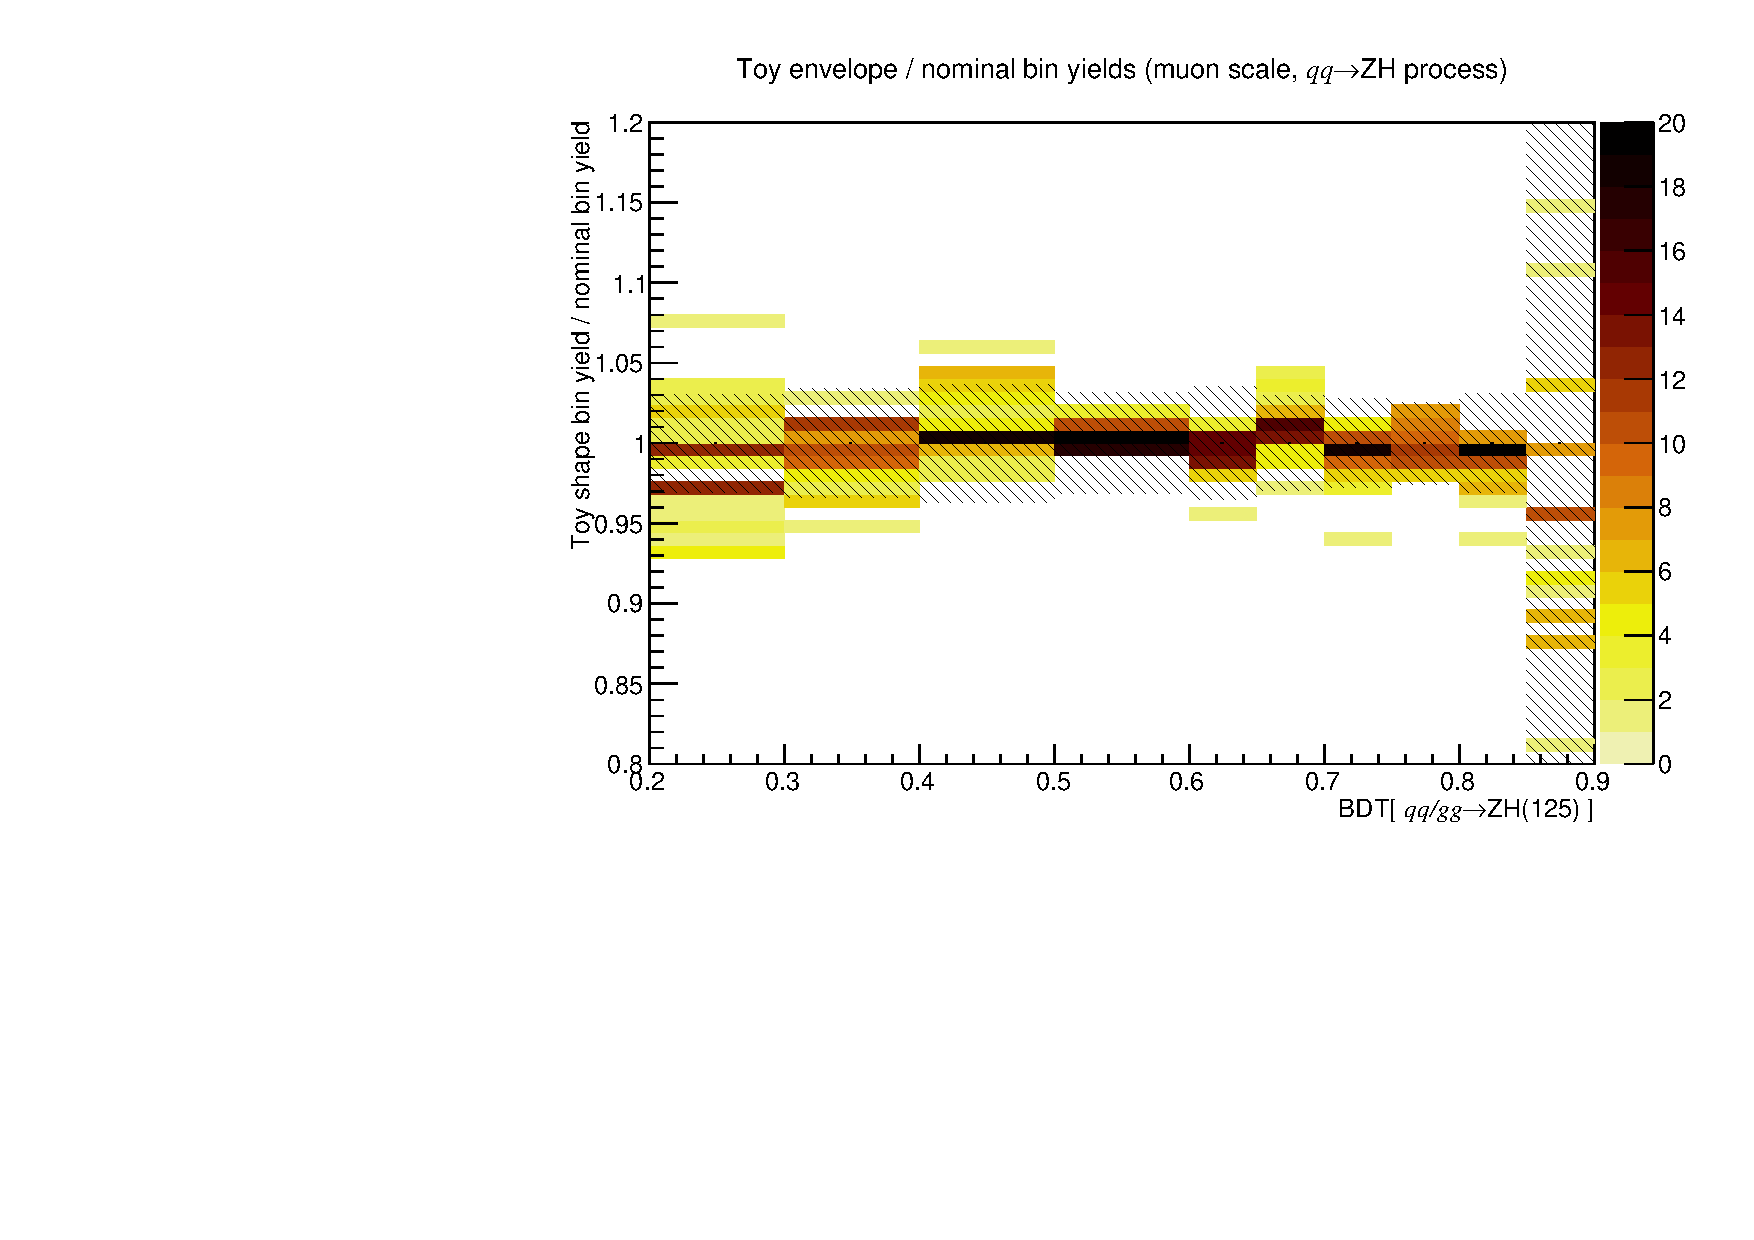
\includegraphics[width=0.48\textwidth]{figures/syst_BDT_ZH_hinv_sm_toyenvelope_muon.pdf}
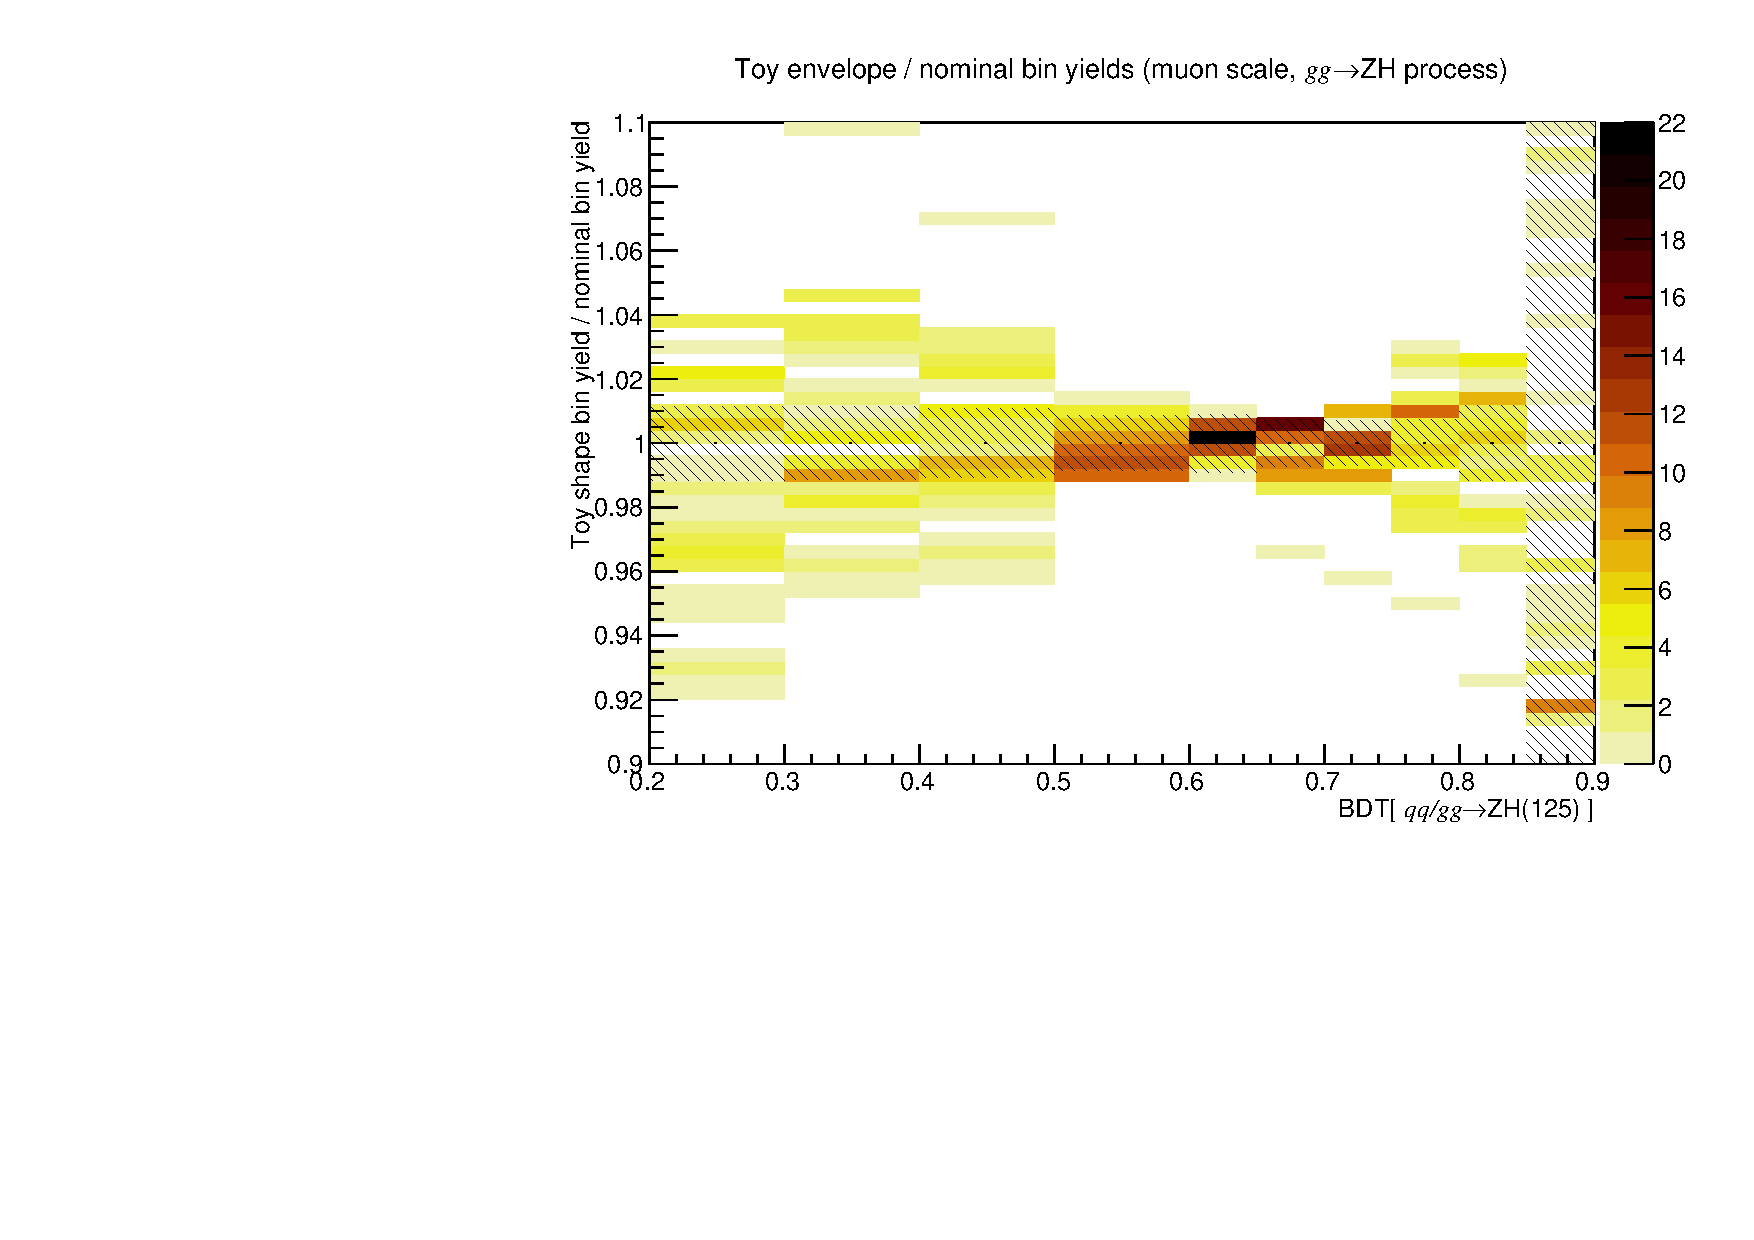
\includegraphics[width=0.48\textwidth]{figures/syst_BDT_ggZH_hinv_toyenvelope_muon.pdf}
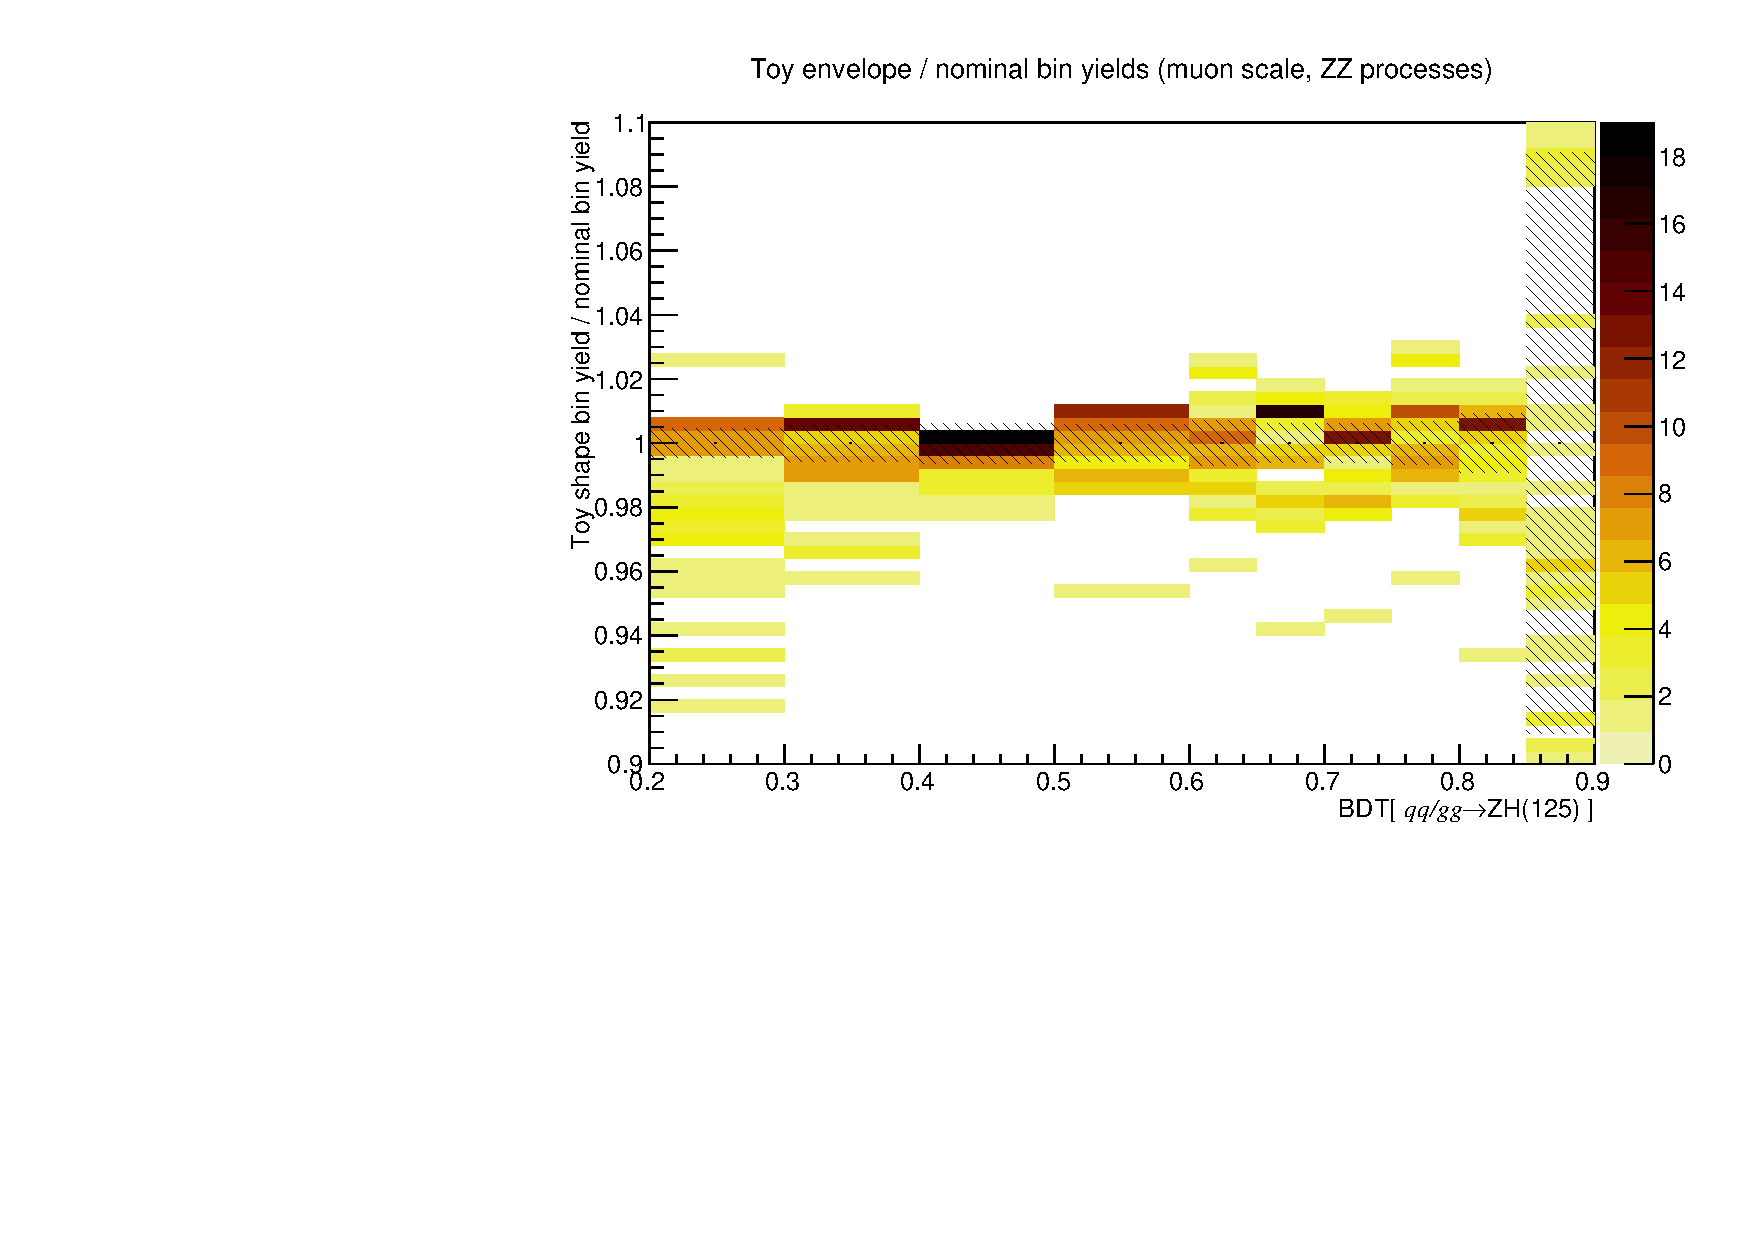
\includegraphics[width=0.48\textwidth]{figures/syst_BDT_ZZ_toyenvelope_muon.pdf}
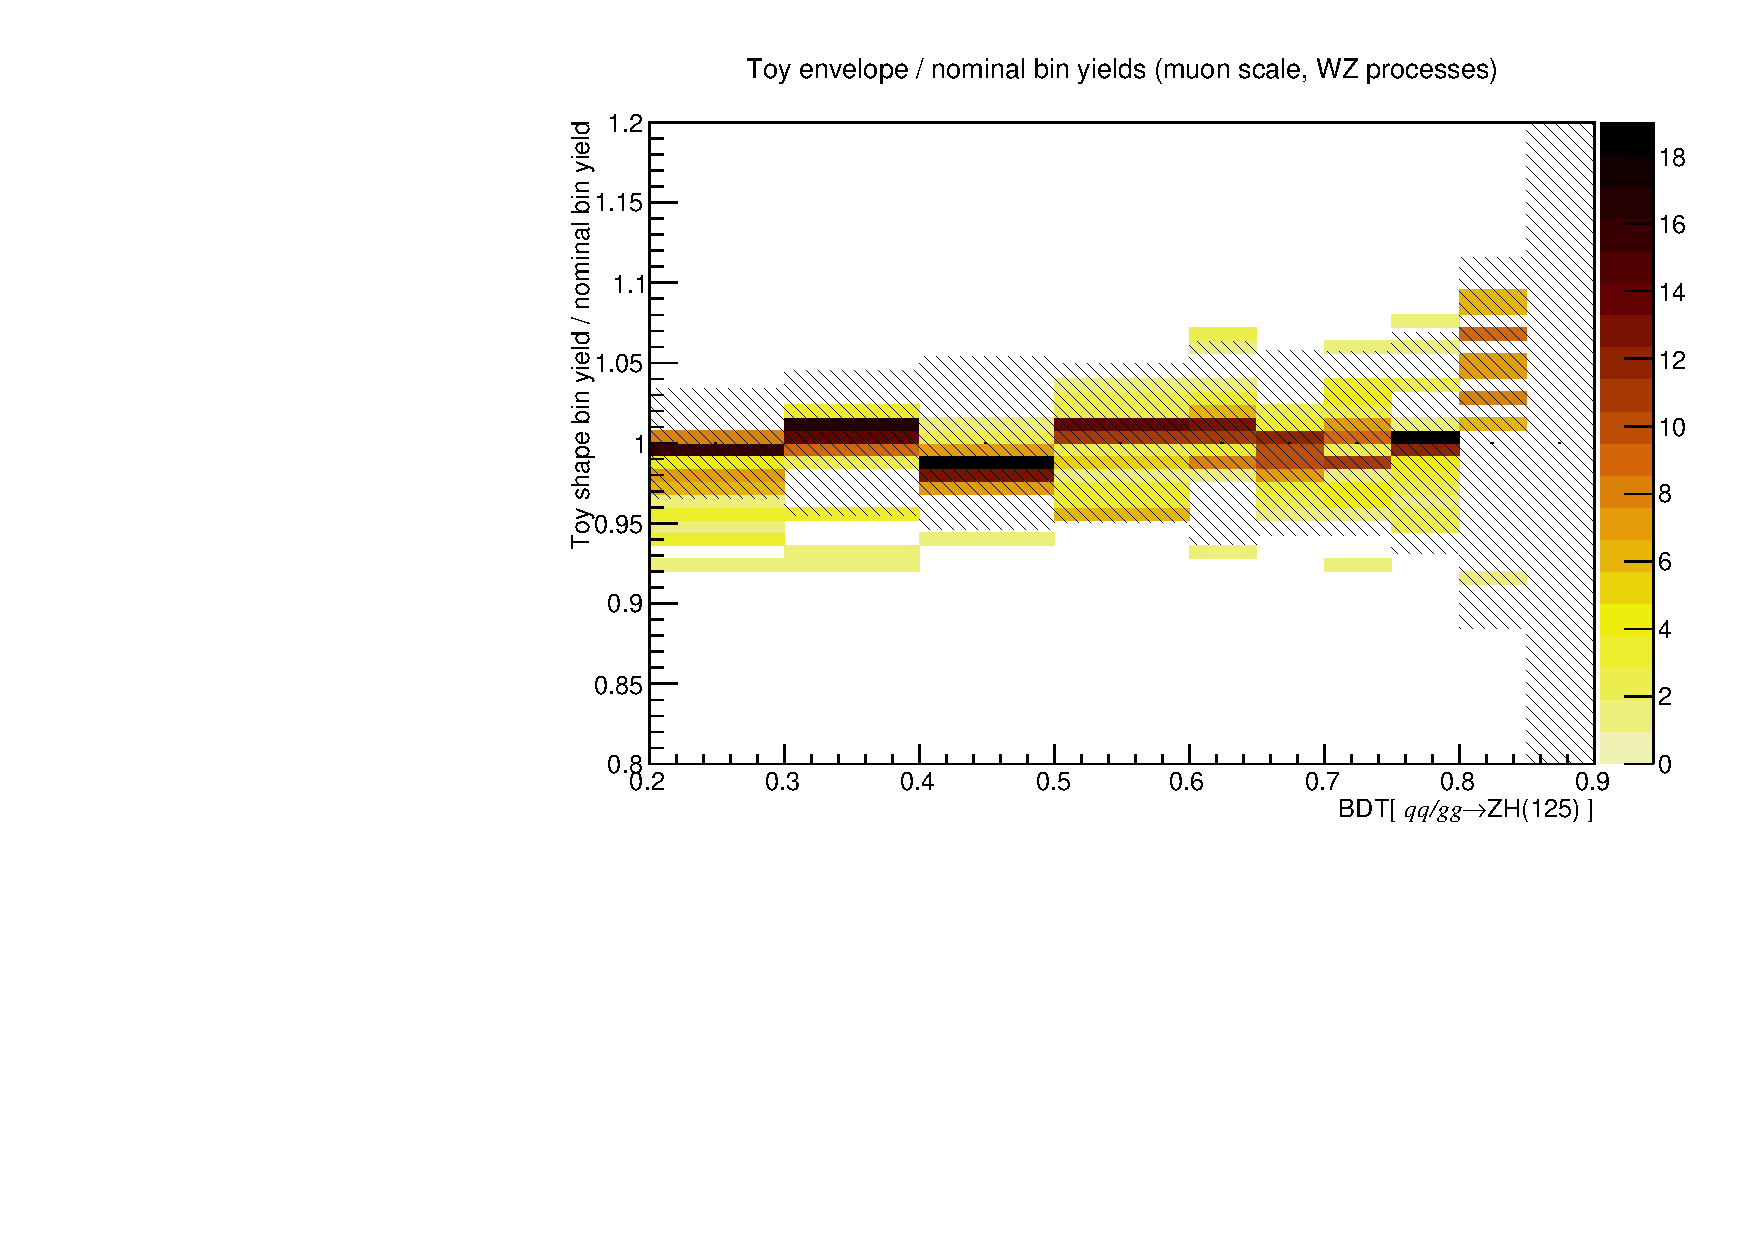
\includegraphics[width=0.48\textwidth]{figures/syst_BDT_WZ_toyenvelope_muon.pdf}
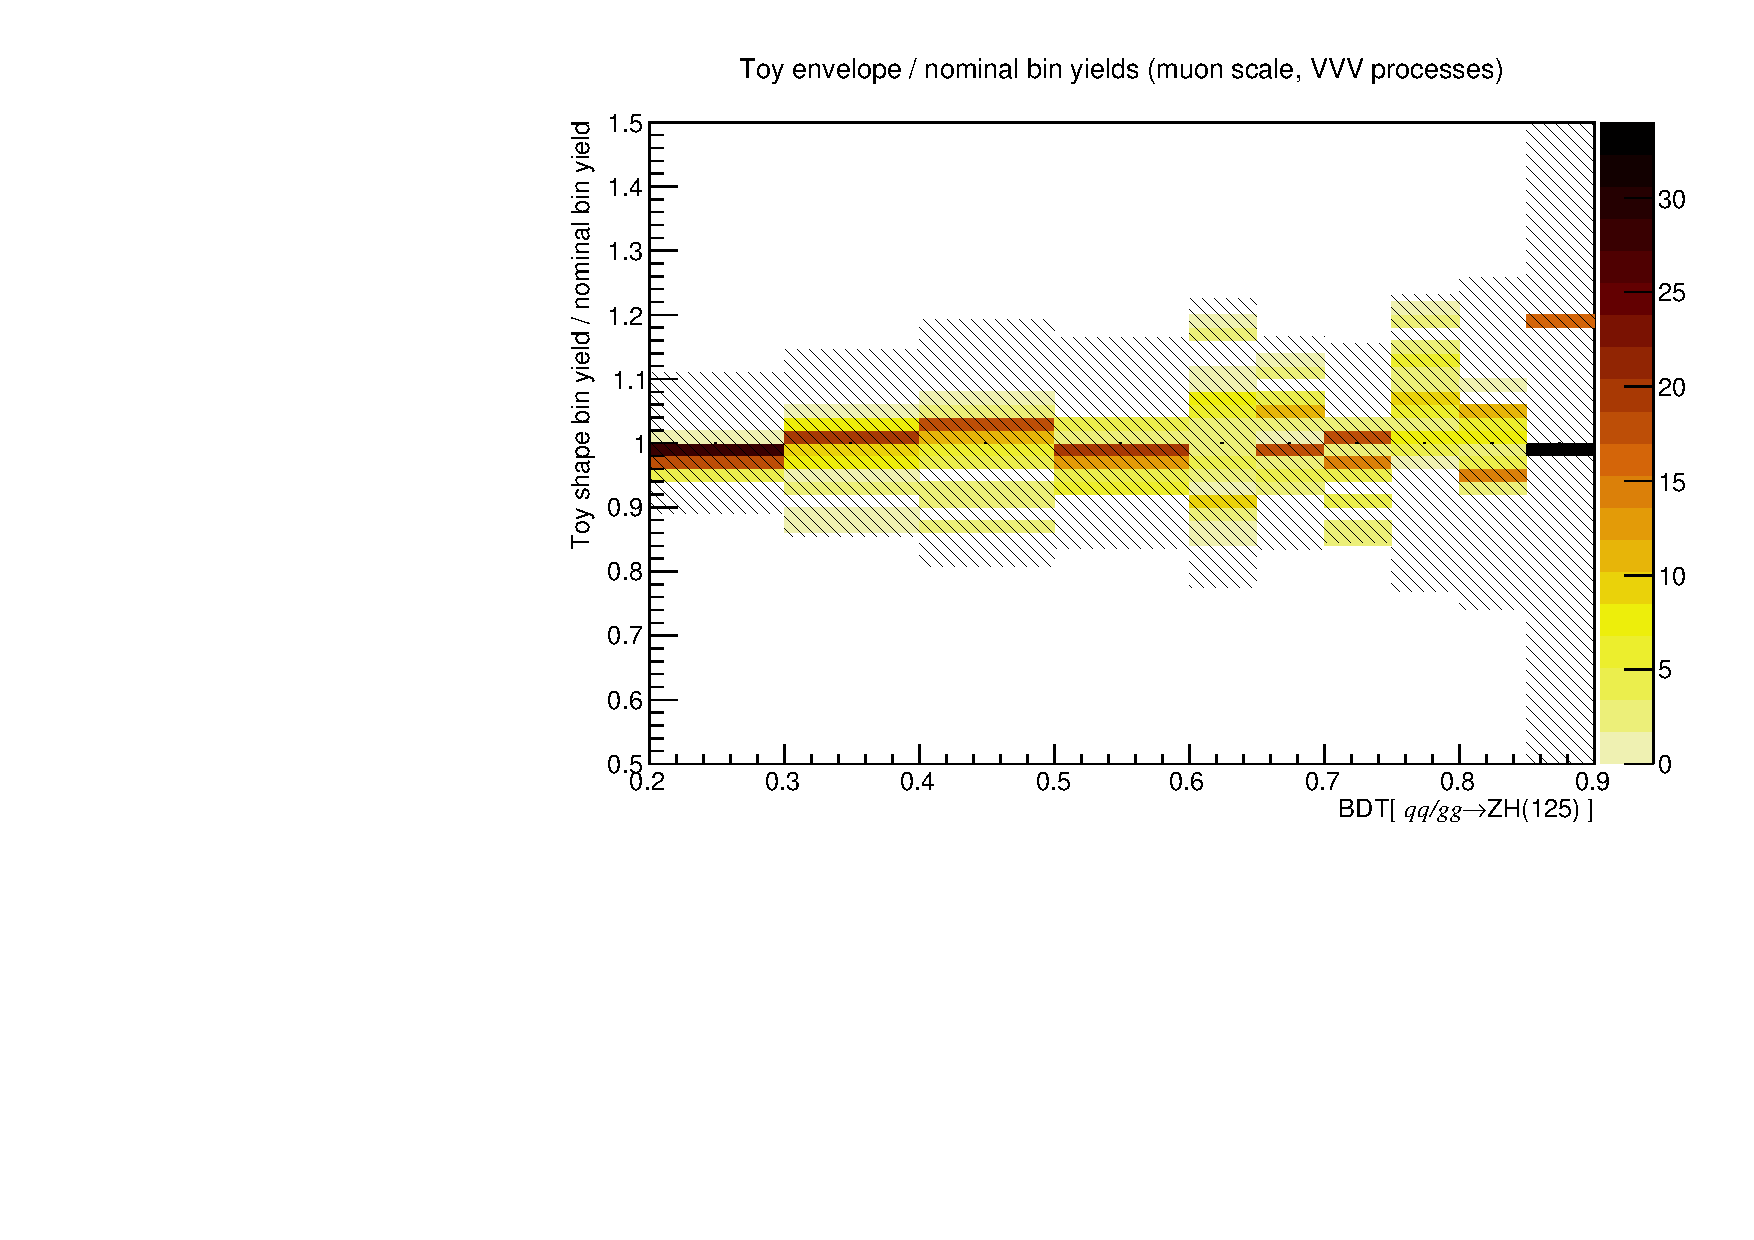
\includegraphics[width=0.48\textwidth]{figures/syst_BDT_VVV_toyenvelope_muon.pdf}
\caption{2D maps of the relative toy variations from the nominal BDT shape versus the BDT value, for the muon scale. The hashed bands represent statistical uncertainty on the simulated events.}
\label{fig:bdt_toy_envelopes_muon}
\end{center}
\end{figure}

\begin{figure}[htbp]
\begin{center}
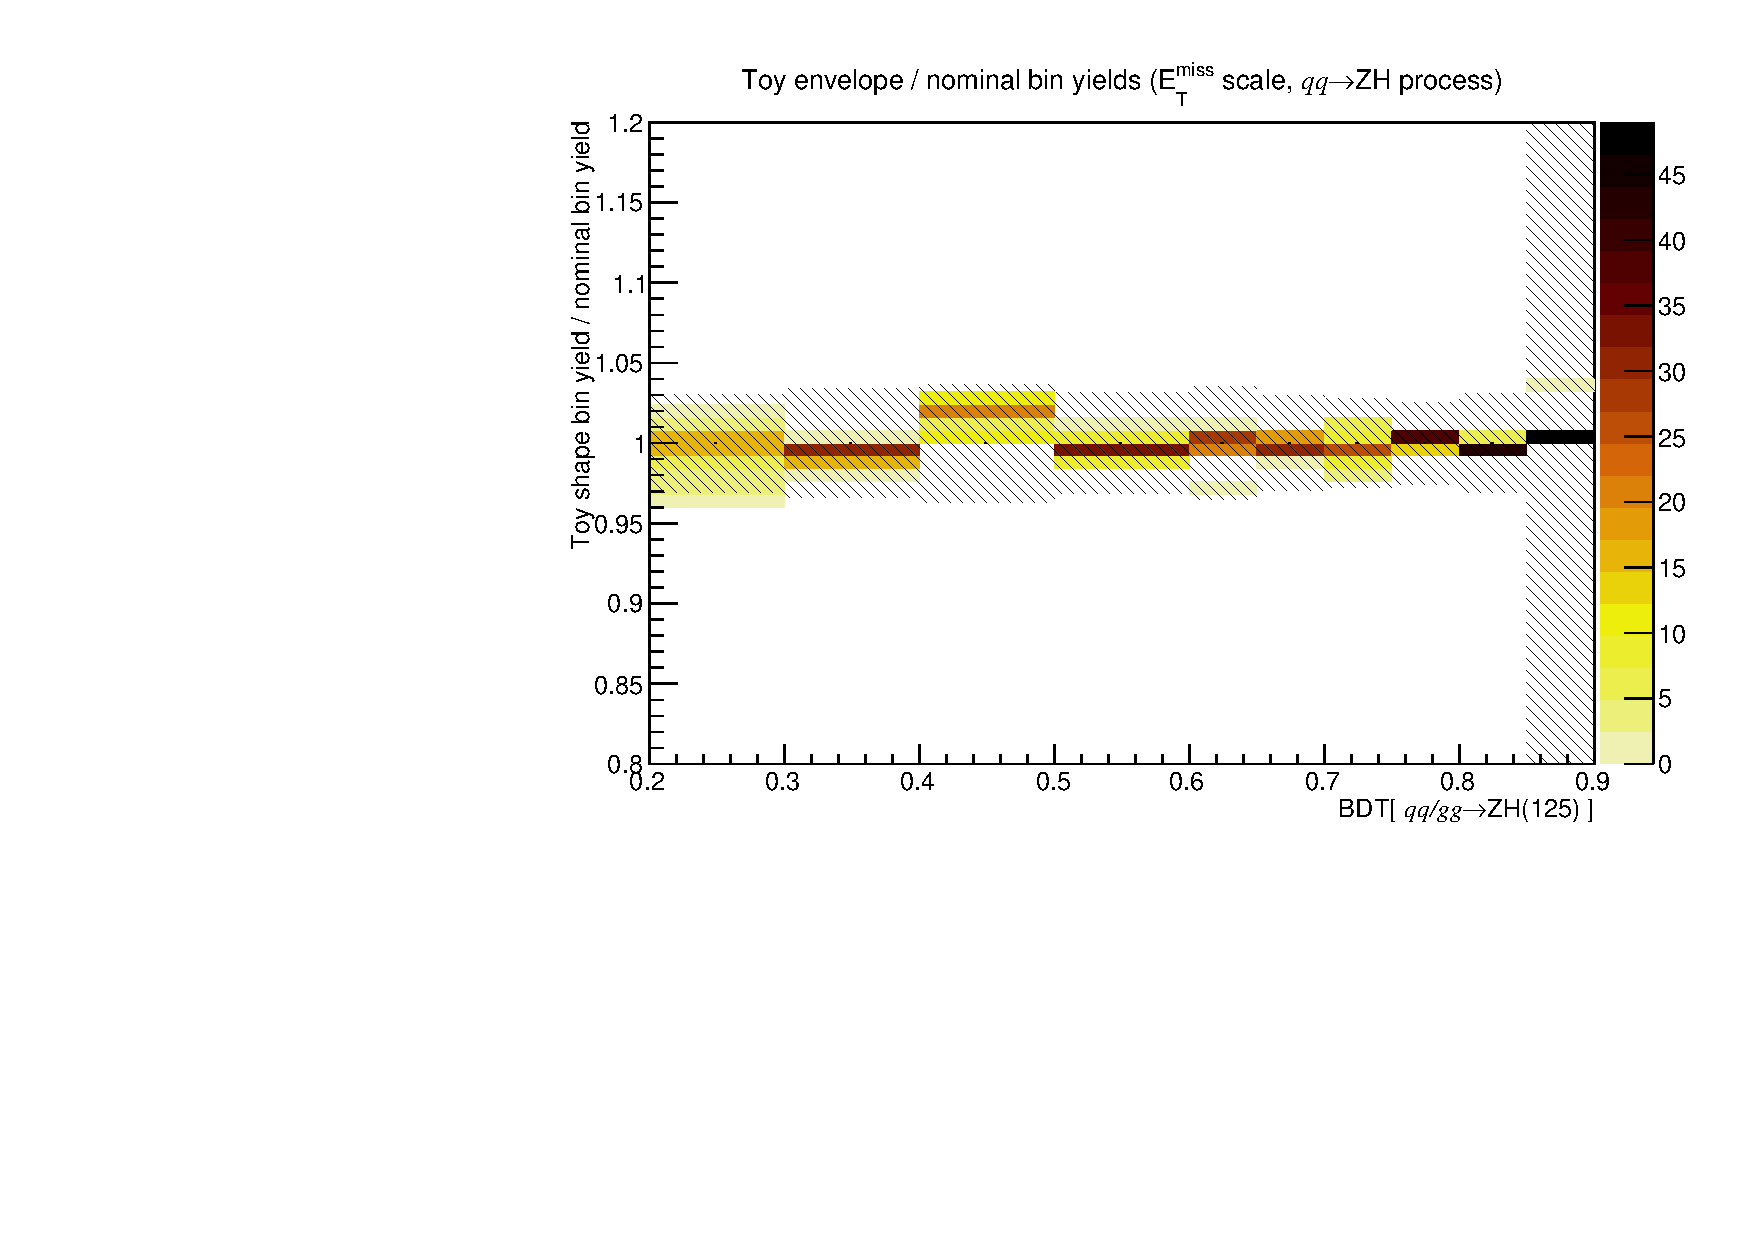
\includegraphics[width=0.48\textwidth]{figures/syst_BDT_ZH_hinv_sm_toyenvelope_MET.pdf}
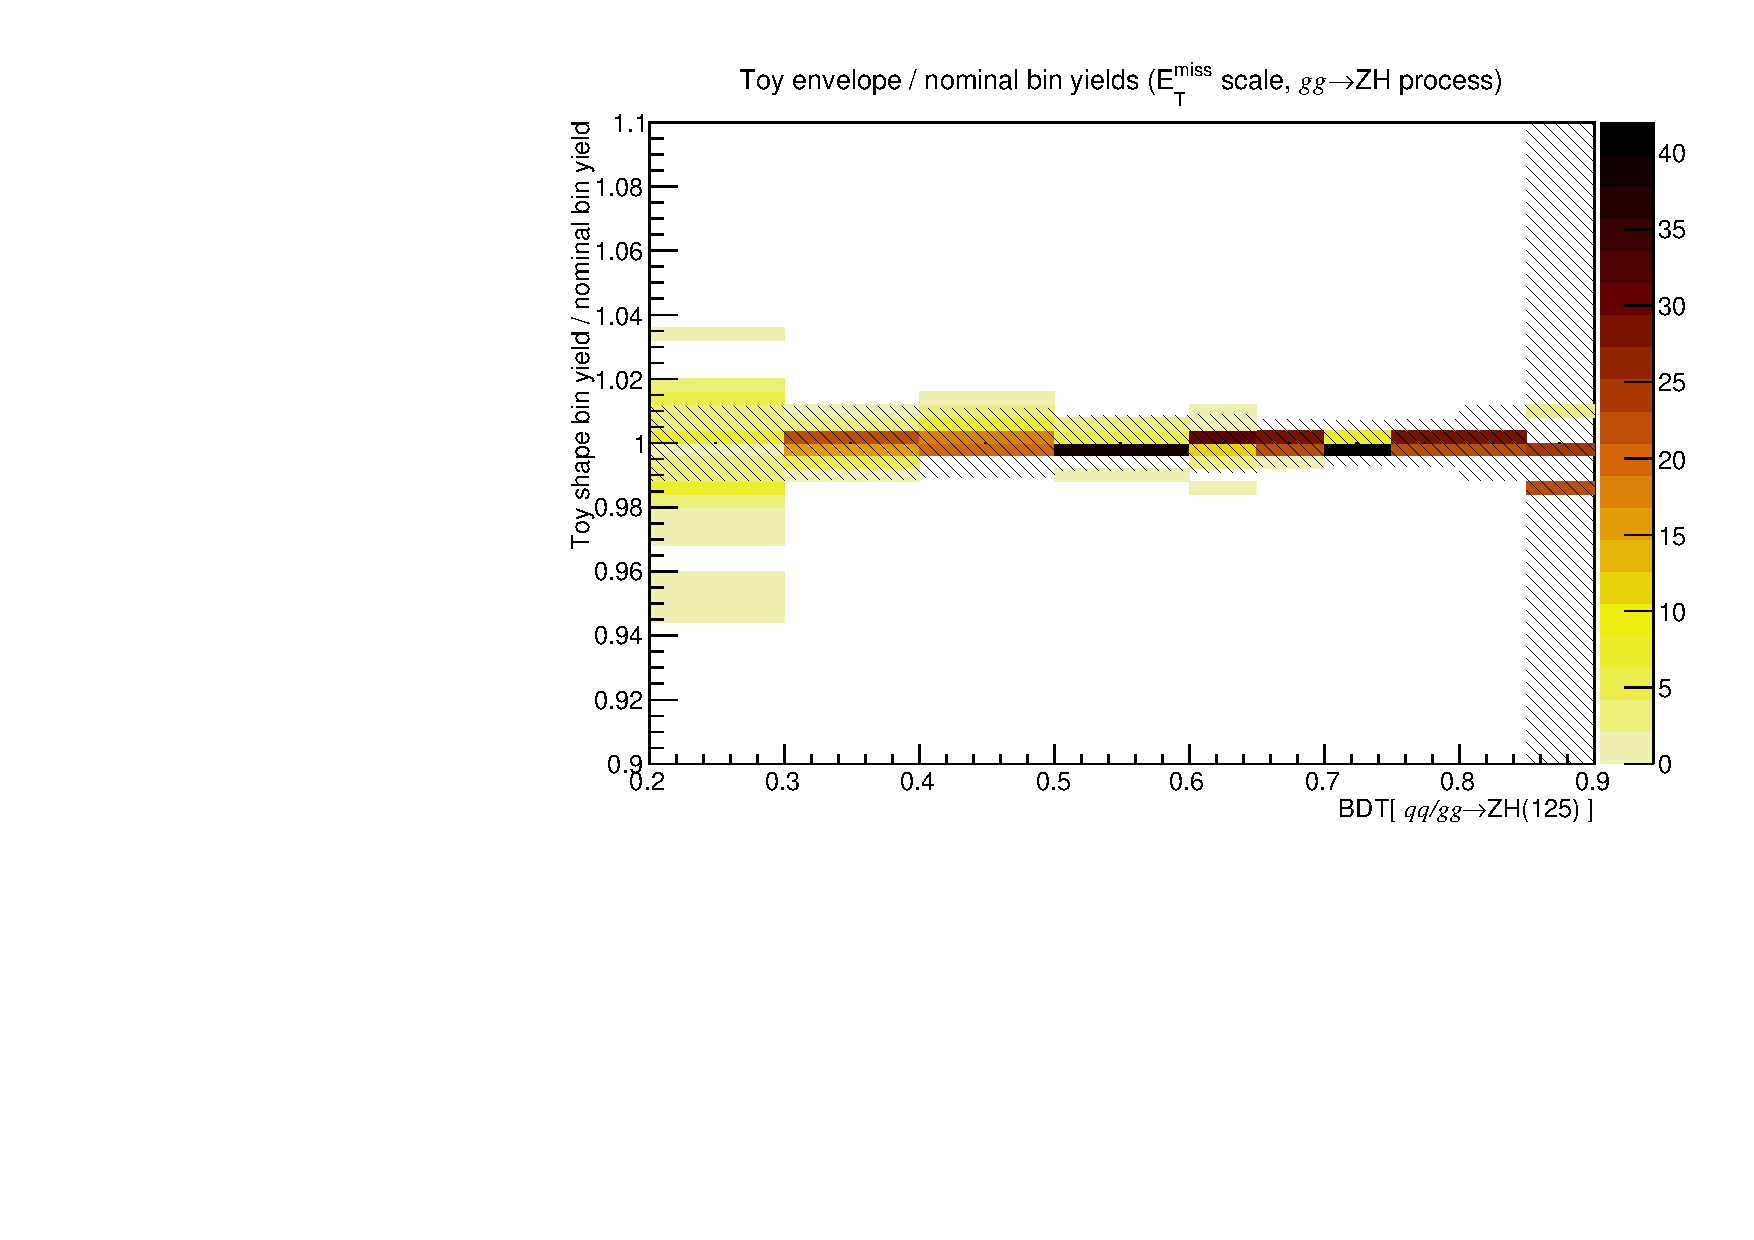
\includegraphics[width=0.48\textwidth]{figures/syst_BDT_ggZH_hinv_toyenvelope_MET.pdf}
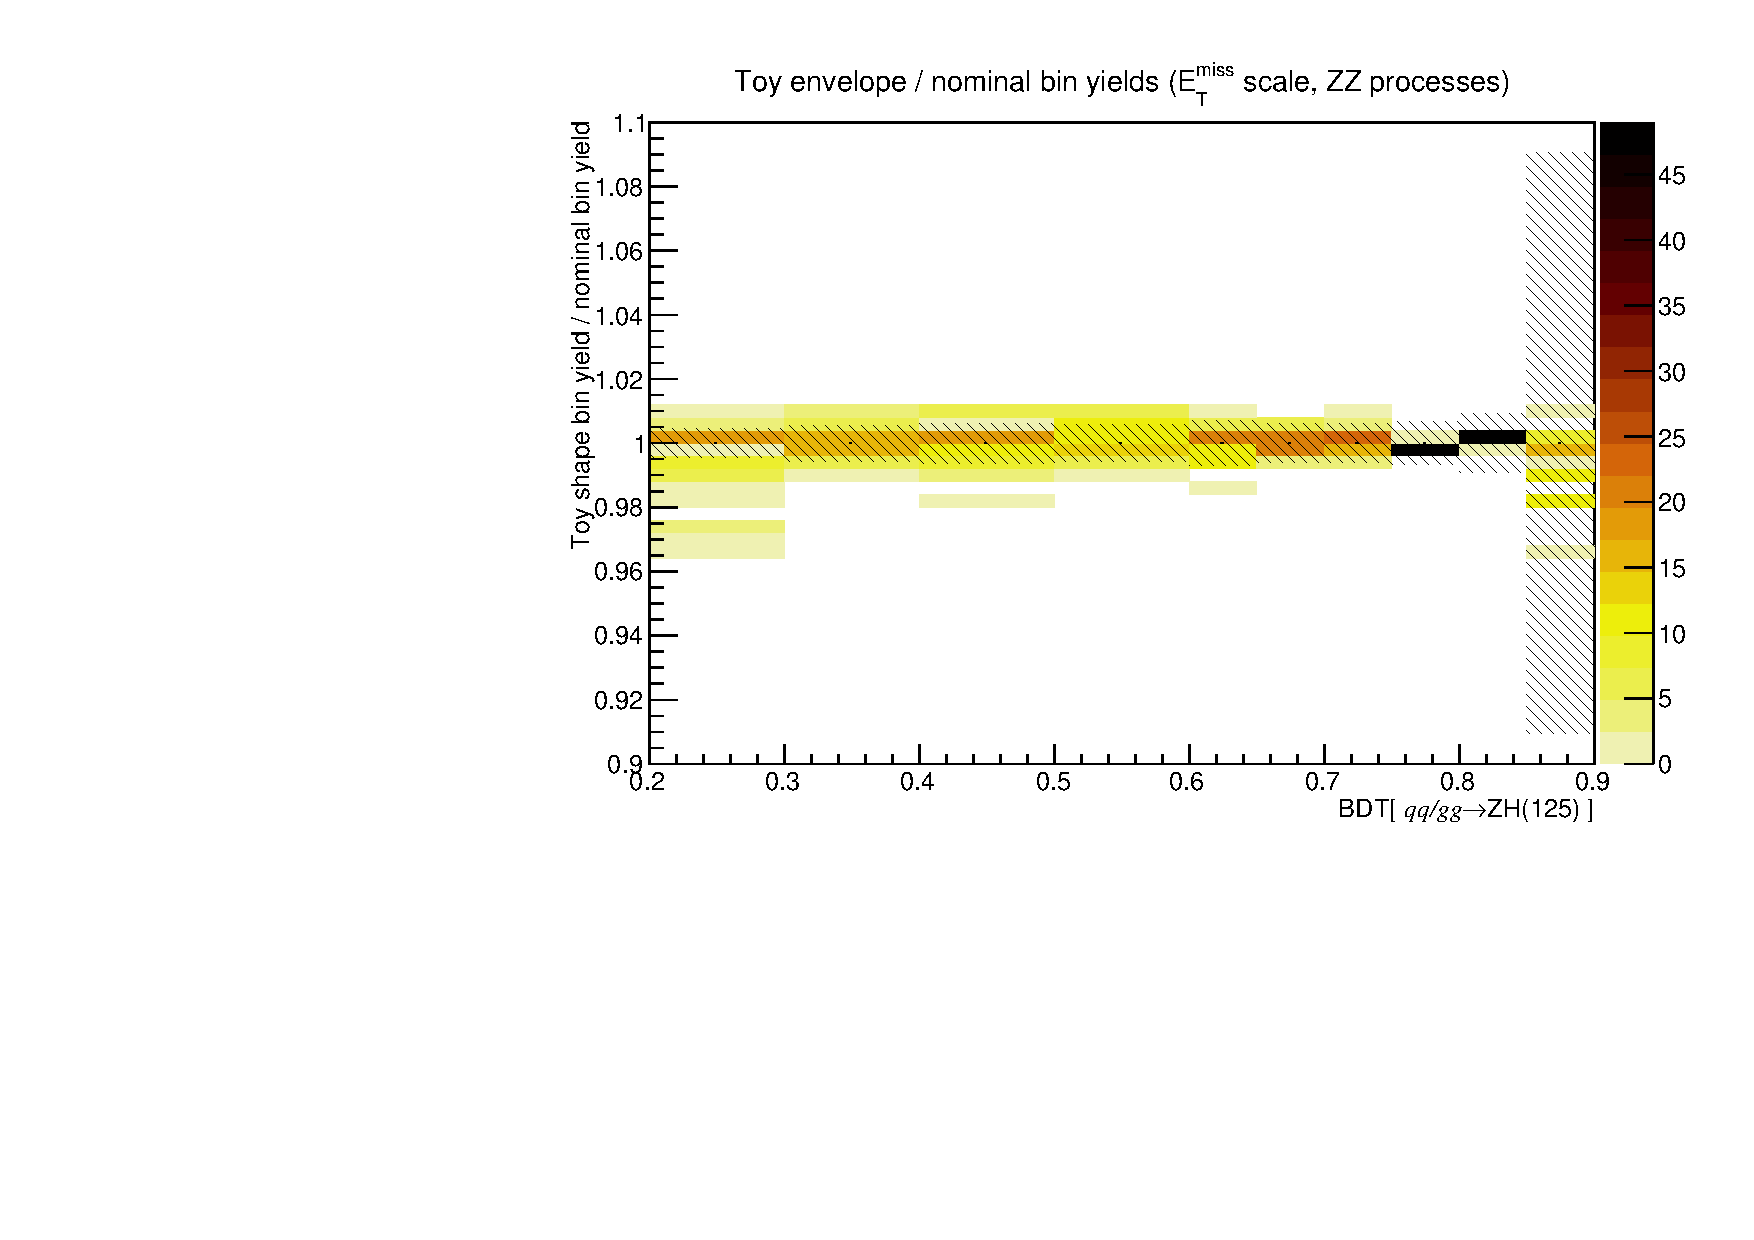
\includegraphics[width=0.48\textwidth]{figures/syst_BDT_ZZ_toyenvelope_MET.pdf}
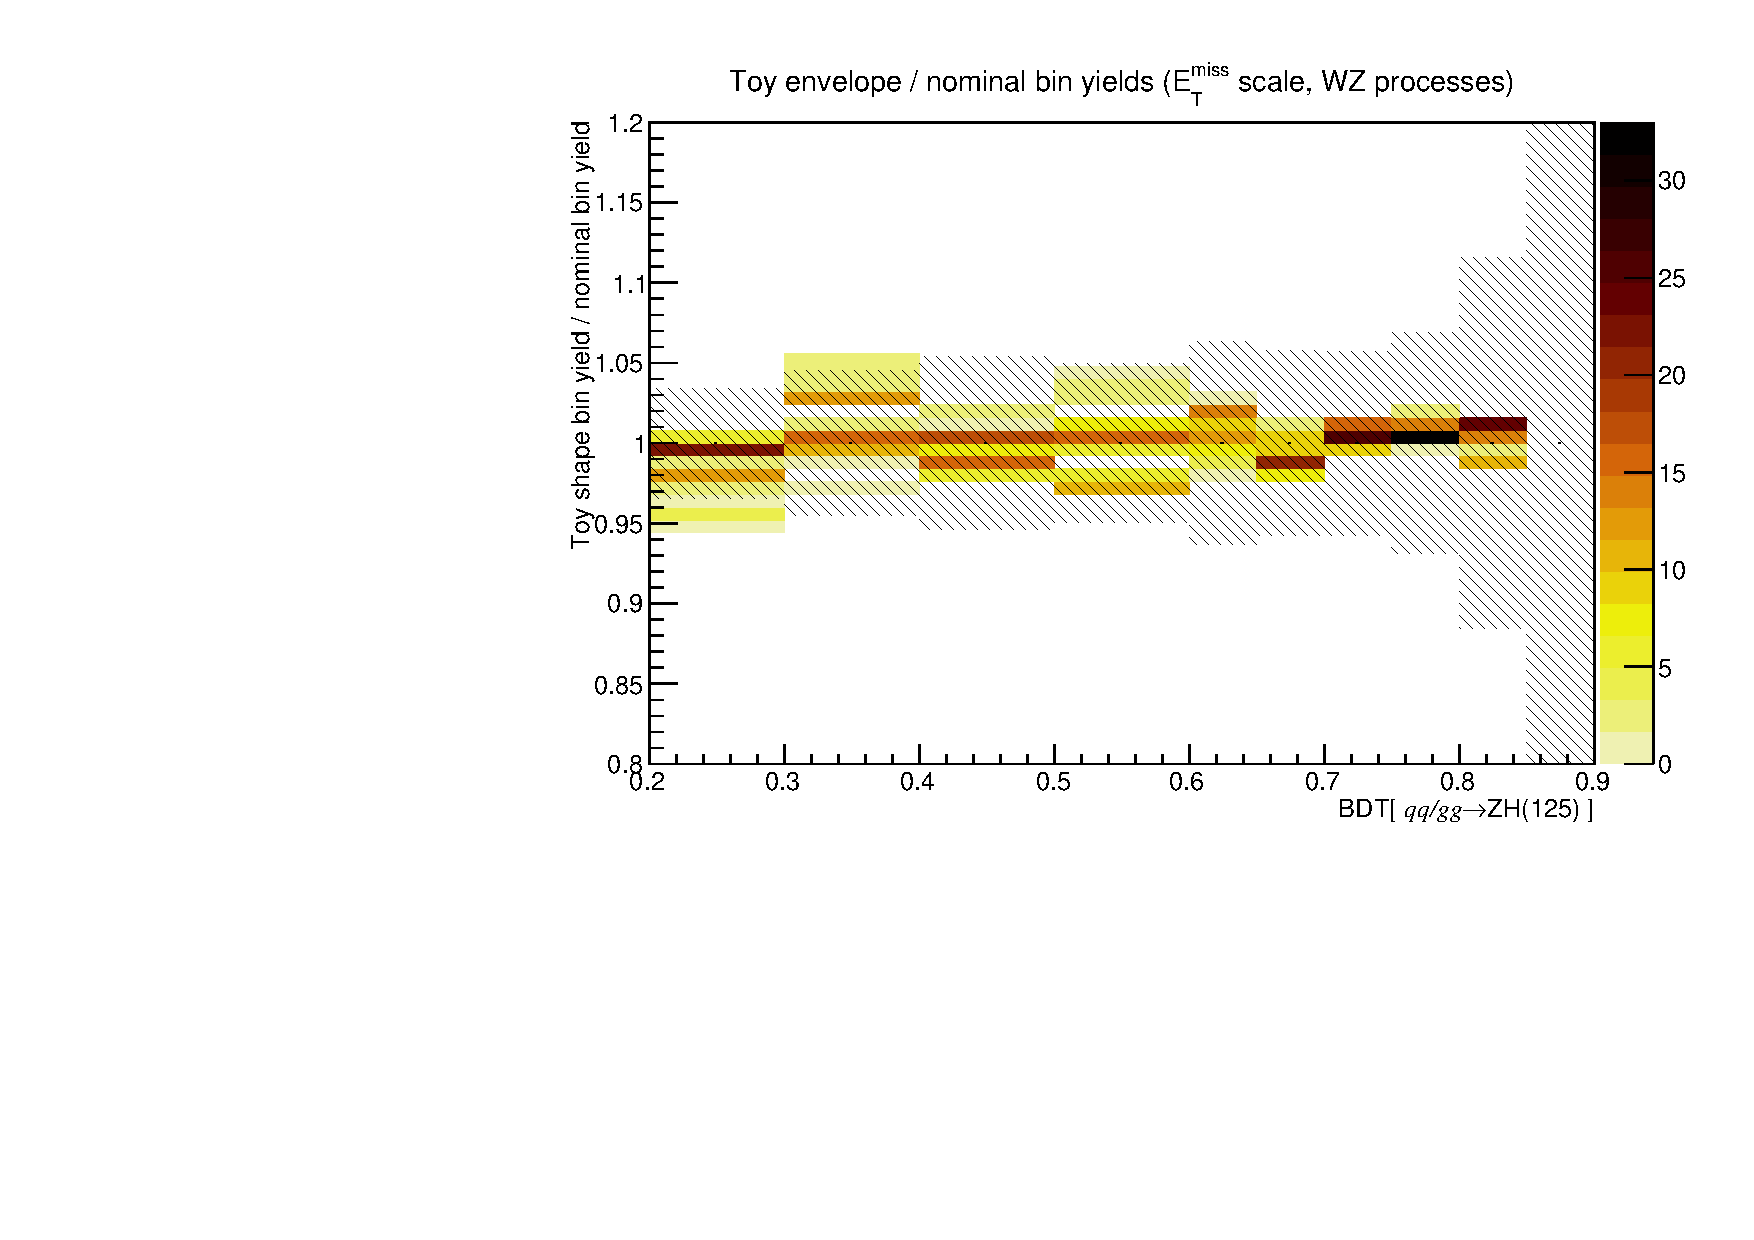
\includegraphics[width=0.48\textwidth]{figures/syst_BDT_WZ_toyenvelope_MET.pdf}
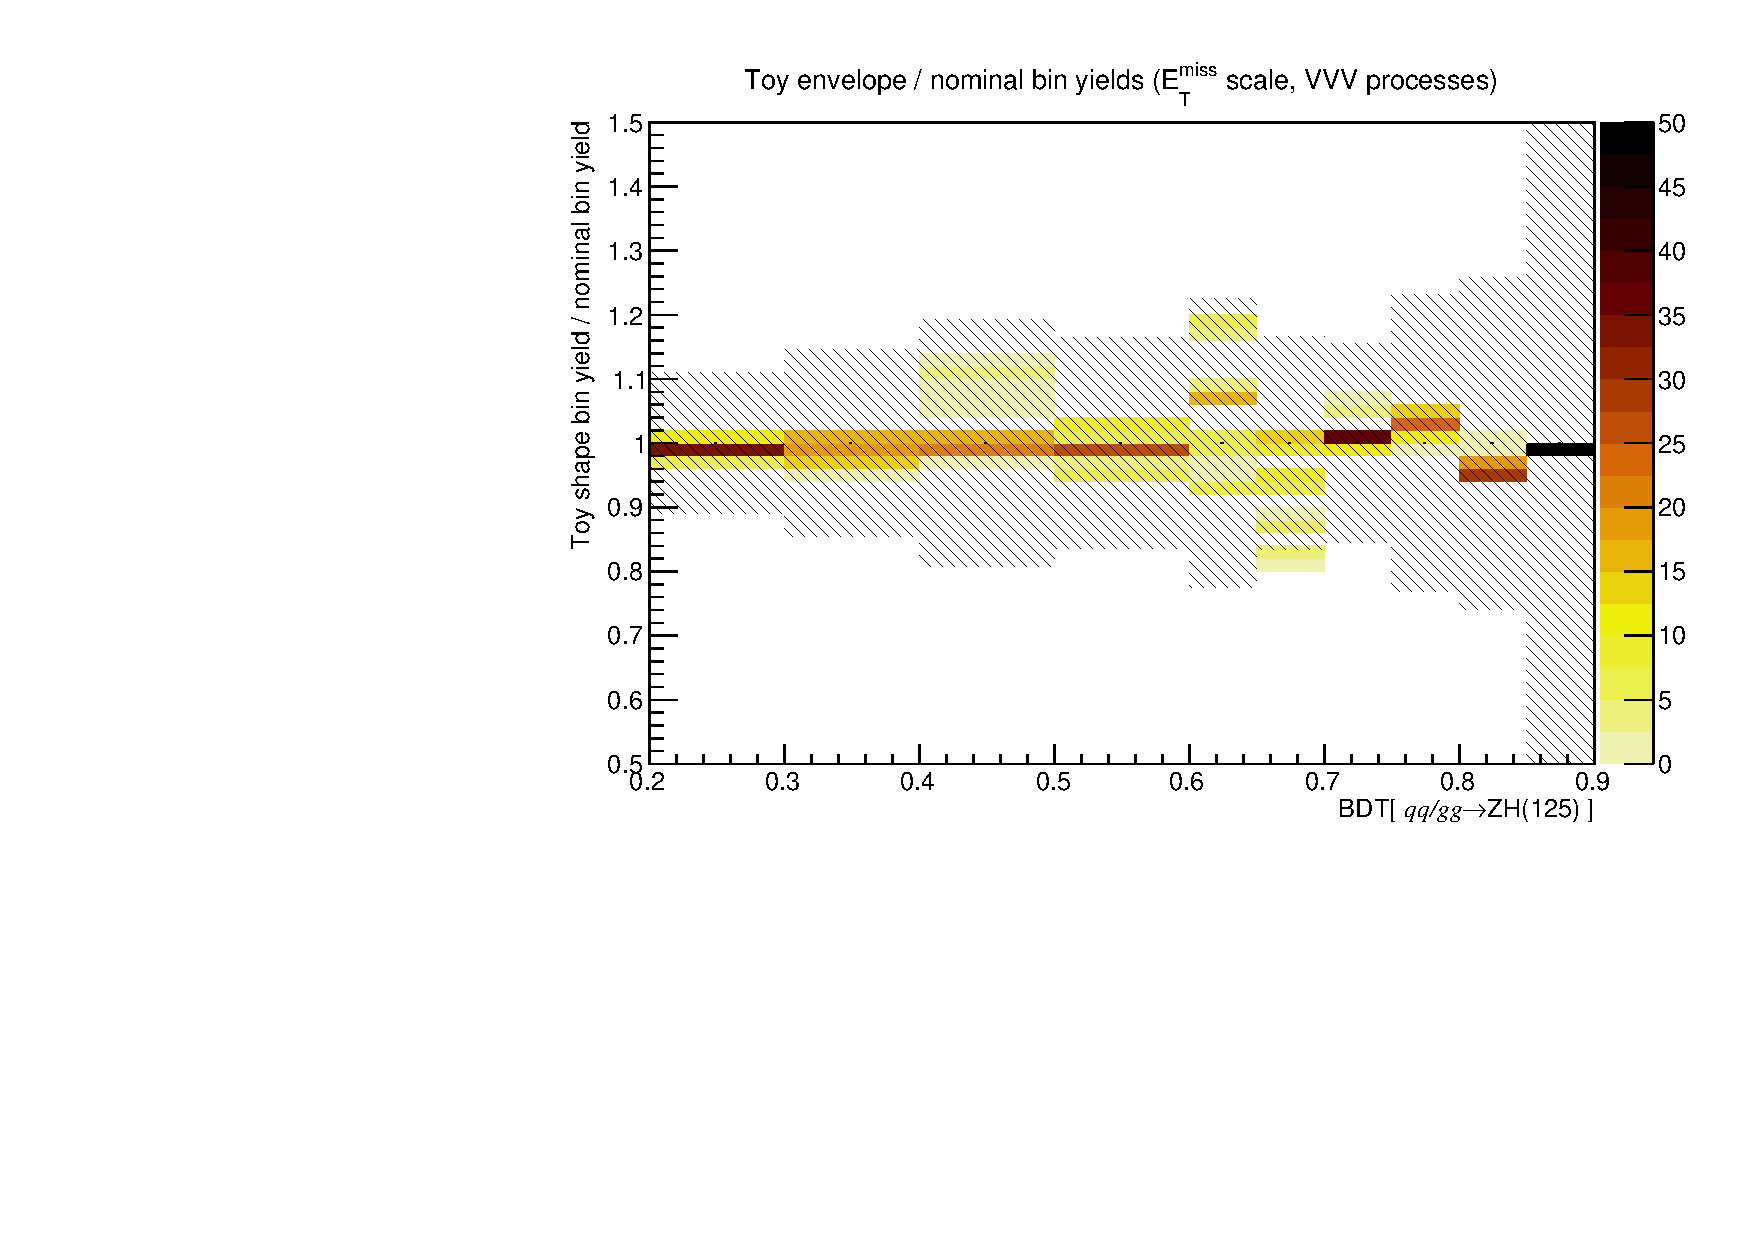
\includegraphics[width=0.48\textwidth]{figures/syst_BDT_VVV_toyenvelope_MET.pdf}
\caption{2D maps of the relative toy variations from the nominal BDT shape versus the BDT value, for the \met scale due to the JES uncertainty. The hashed bands represent statistical uncertainty on the simulated events.}
\label{fig:bdt_toy_envelopes_MET}
\end{center}
\end{figure}

\begin{figure}[htbp]
\begin{center}
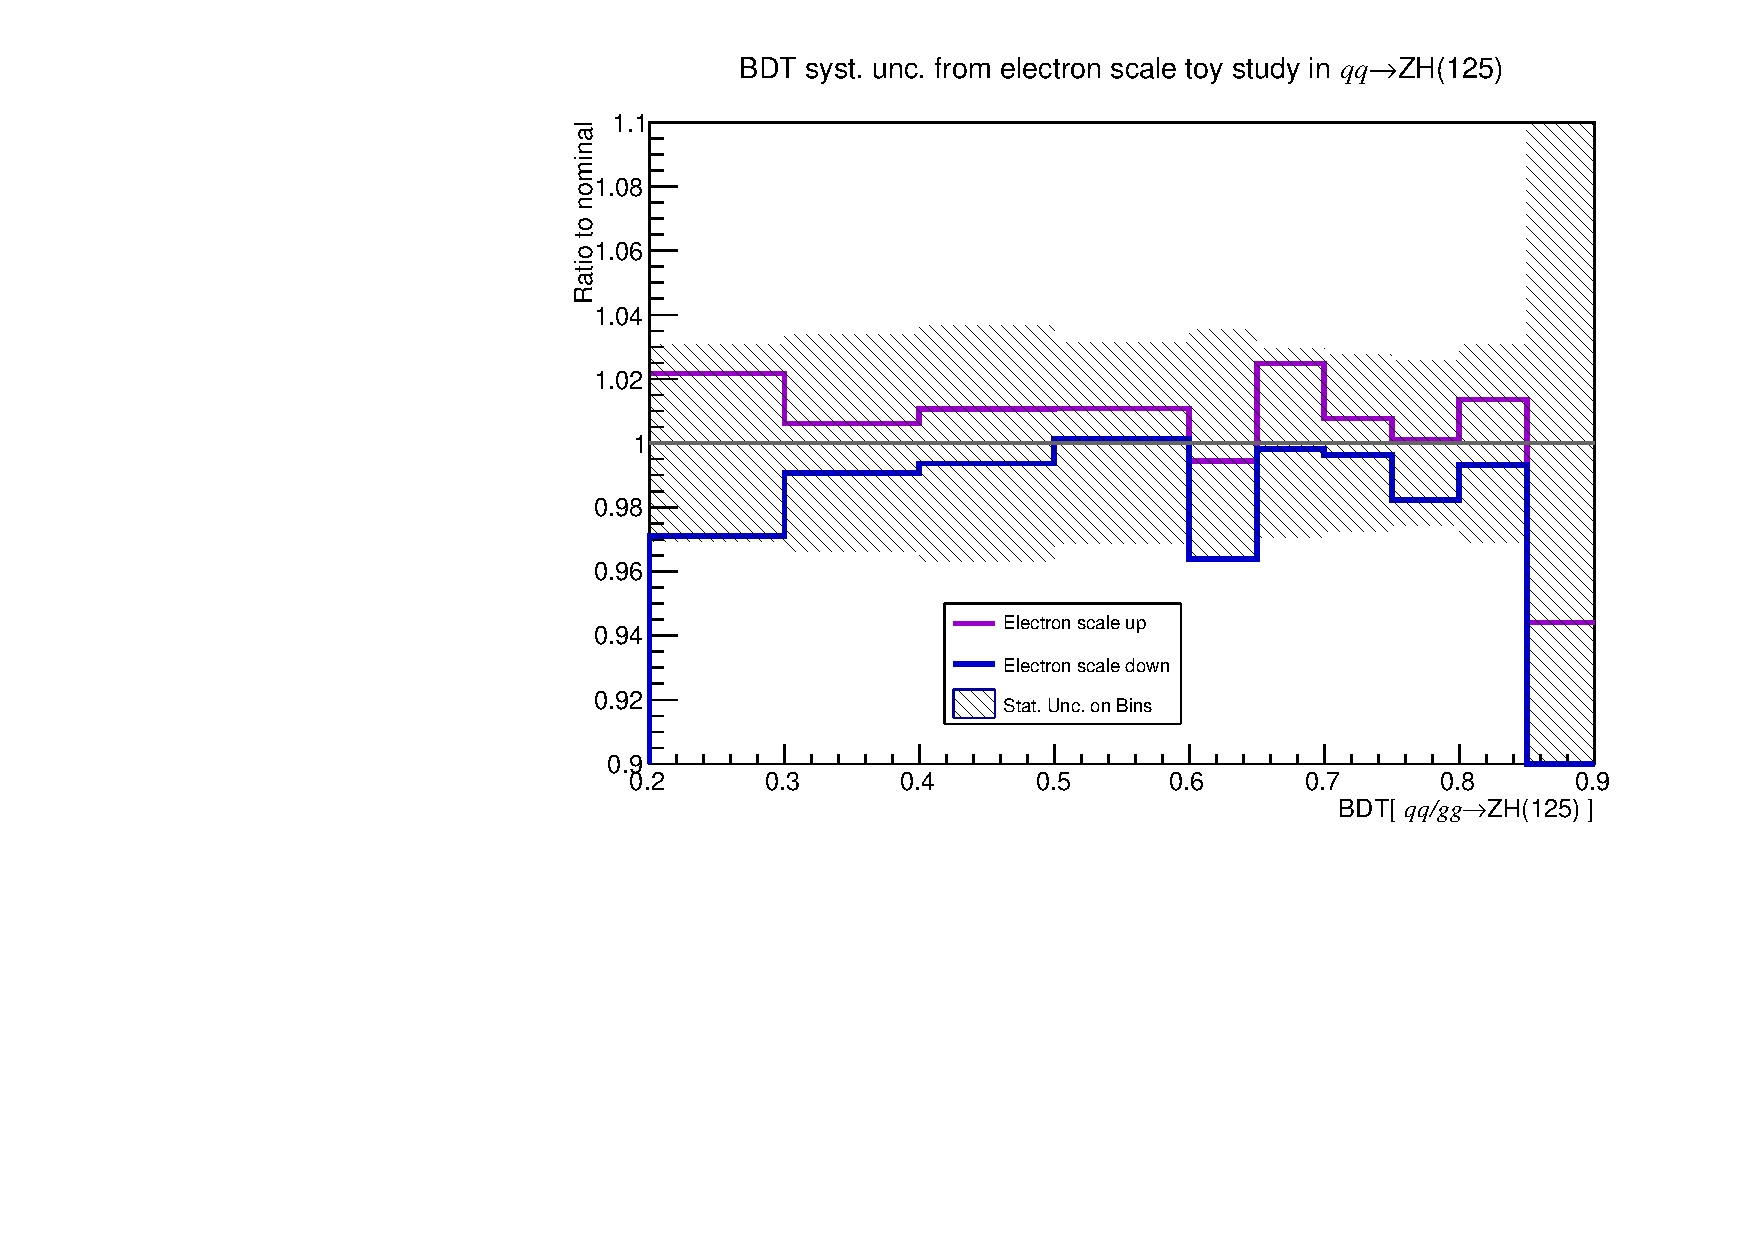
\includegraphics[width=0.48\textwidth]{figures/syst_BDT_ZH_hinv_sm_toys_electron.pdf}
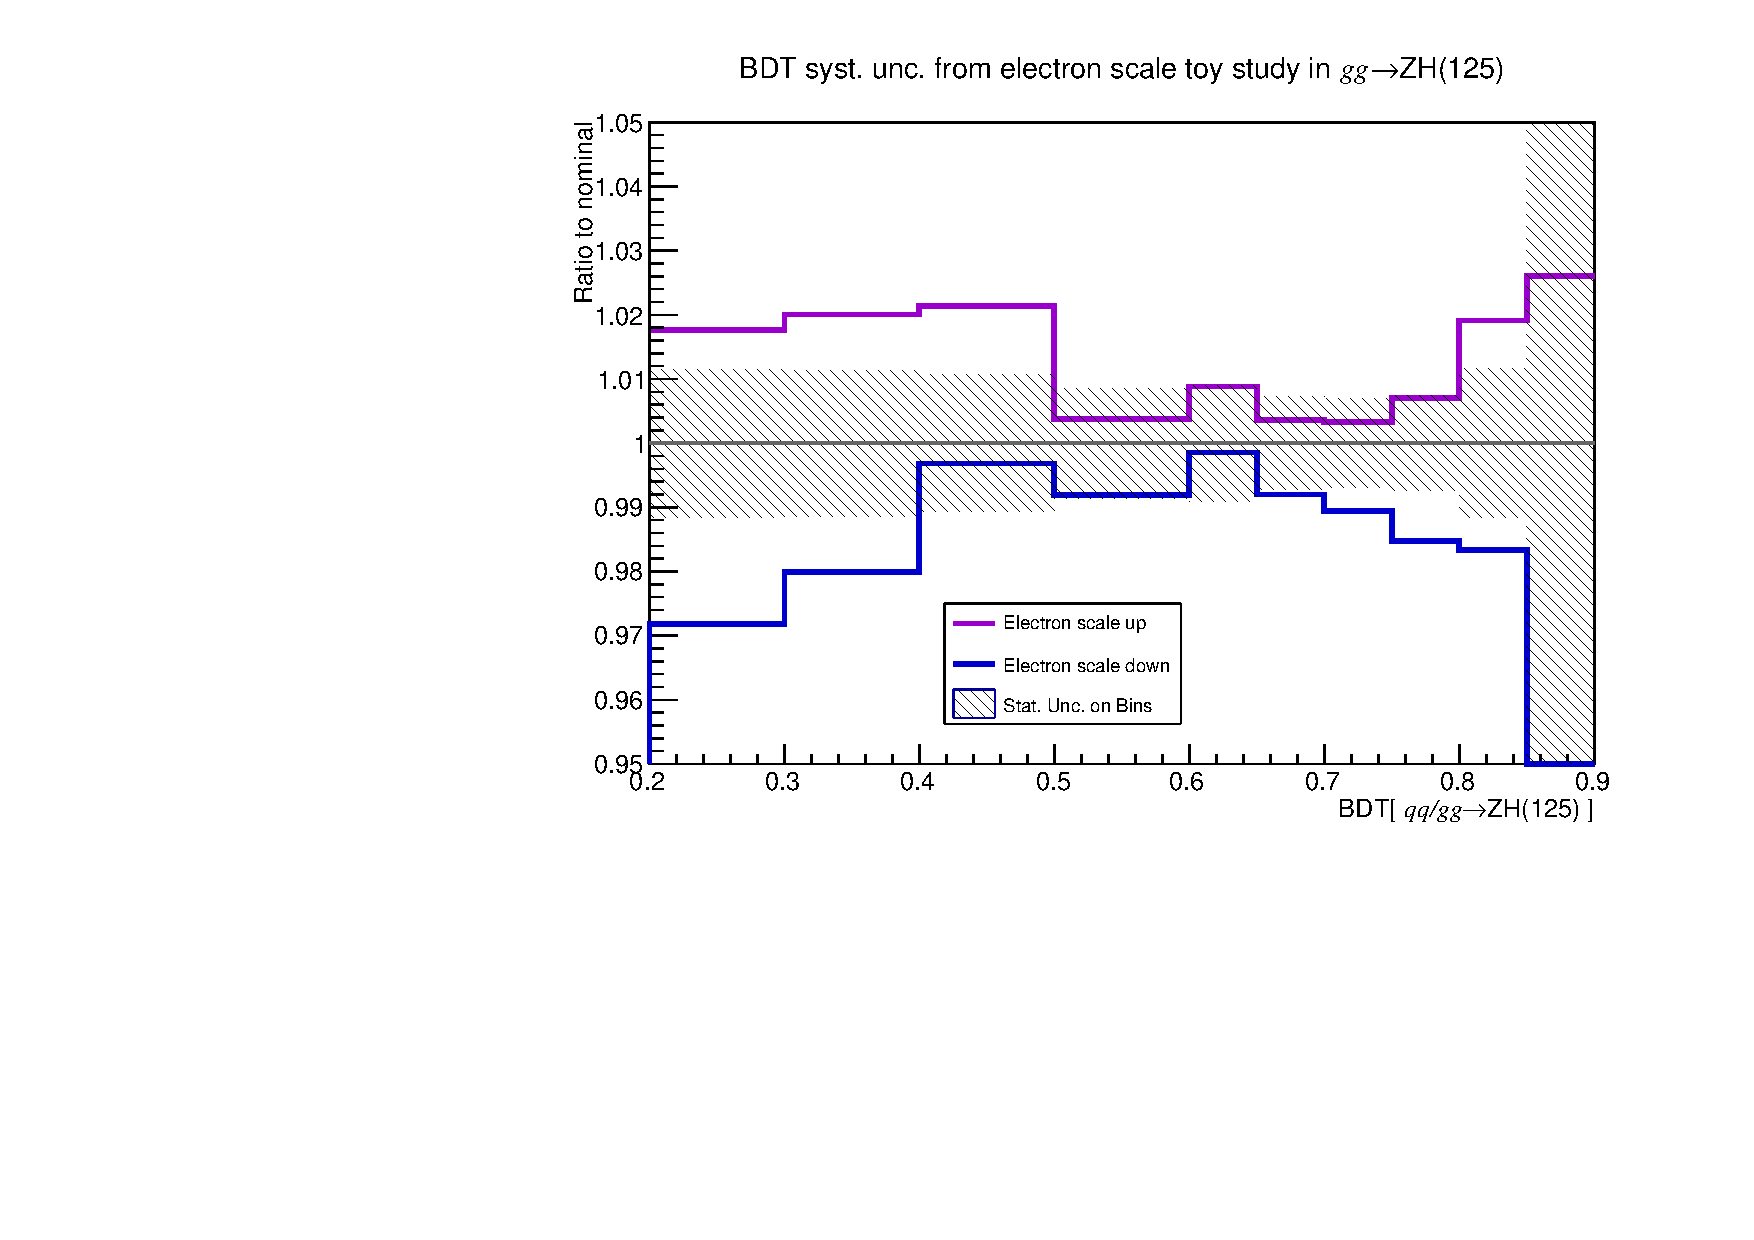
\includegraphics[width=0.48\textwidth]{figures/syst_BDT_ggZH_hinv_toys_electron.pdf}
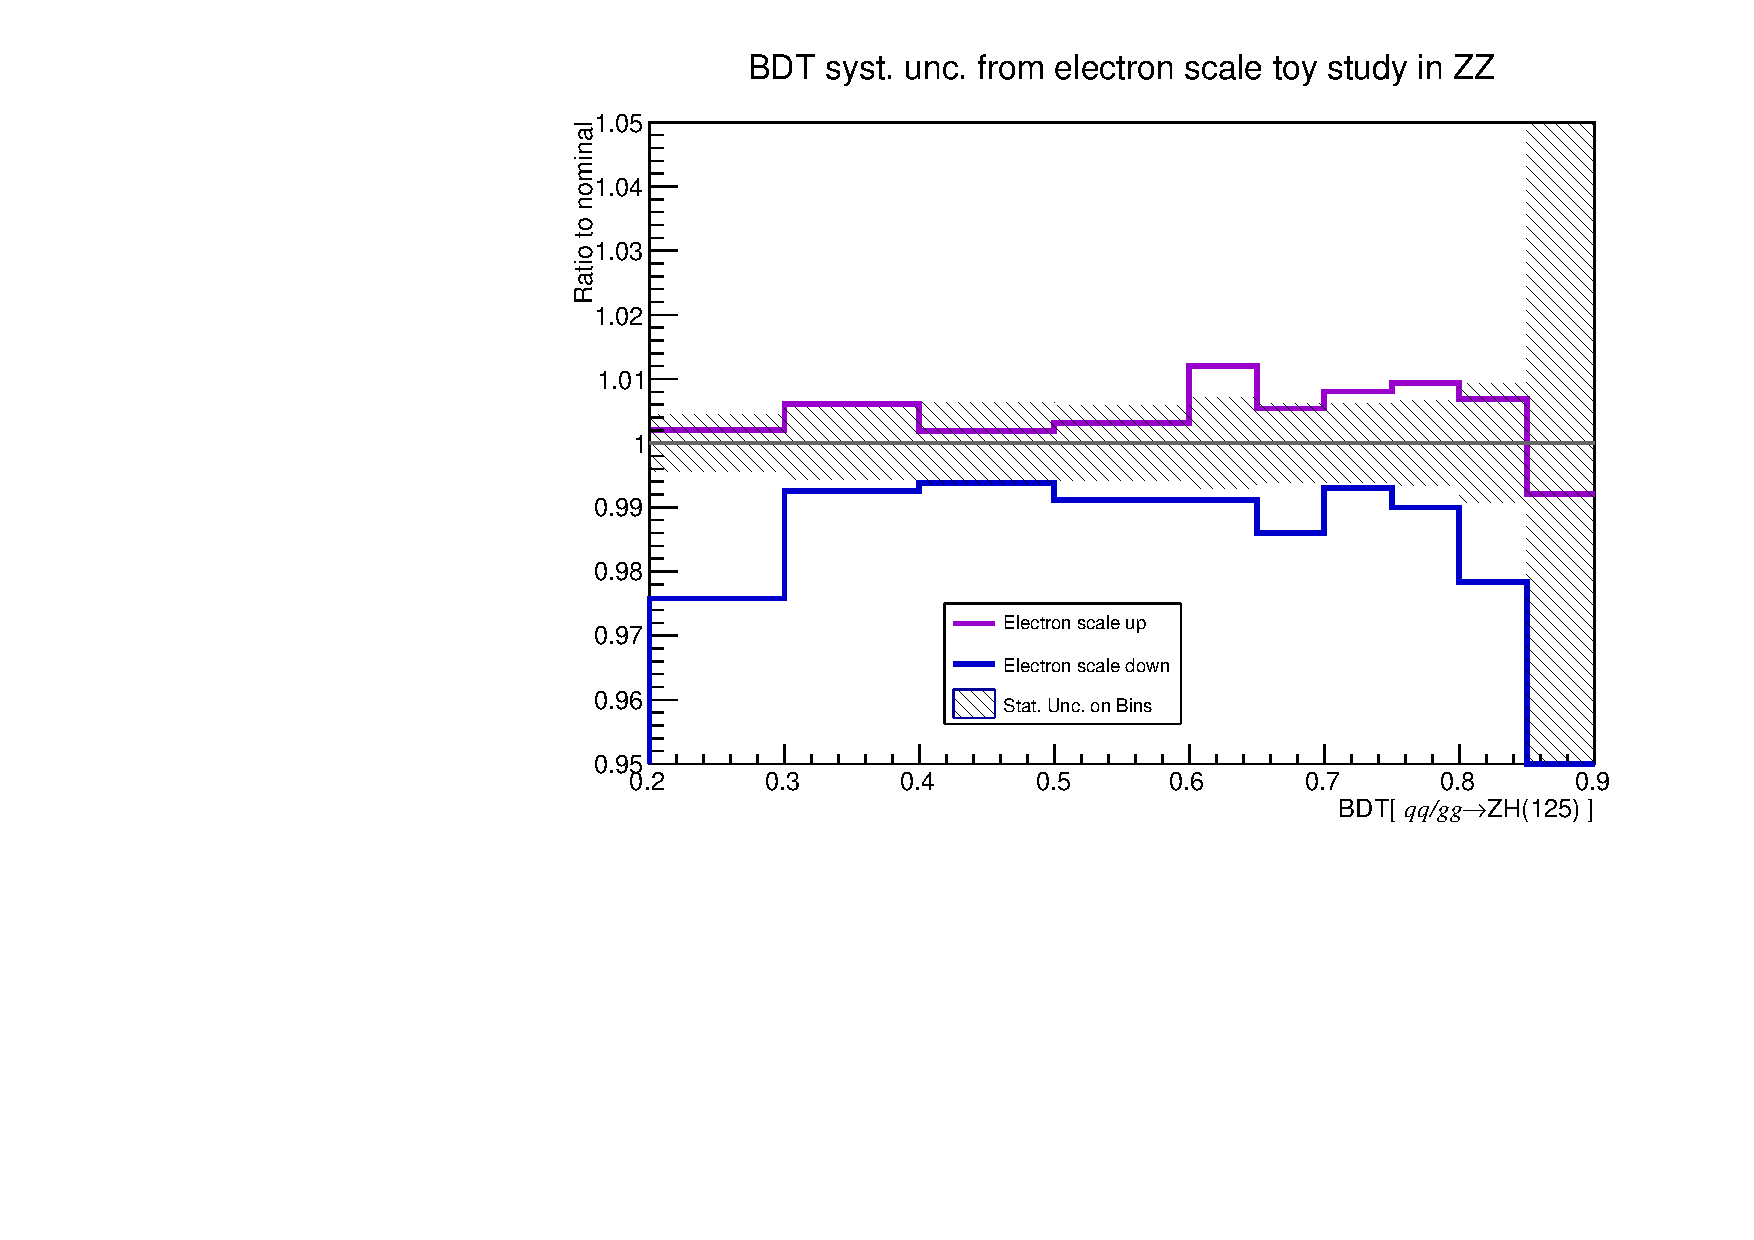
\includegraphics[width=0.48\textwidth]{figures/syst_BDT_ZZ_toys_electron.pdf}
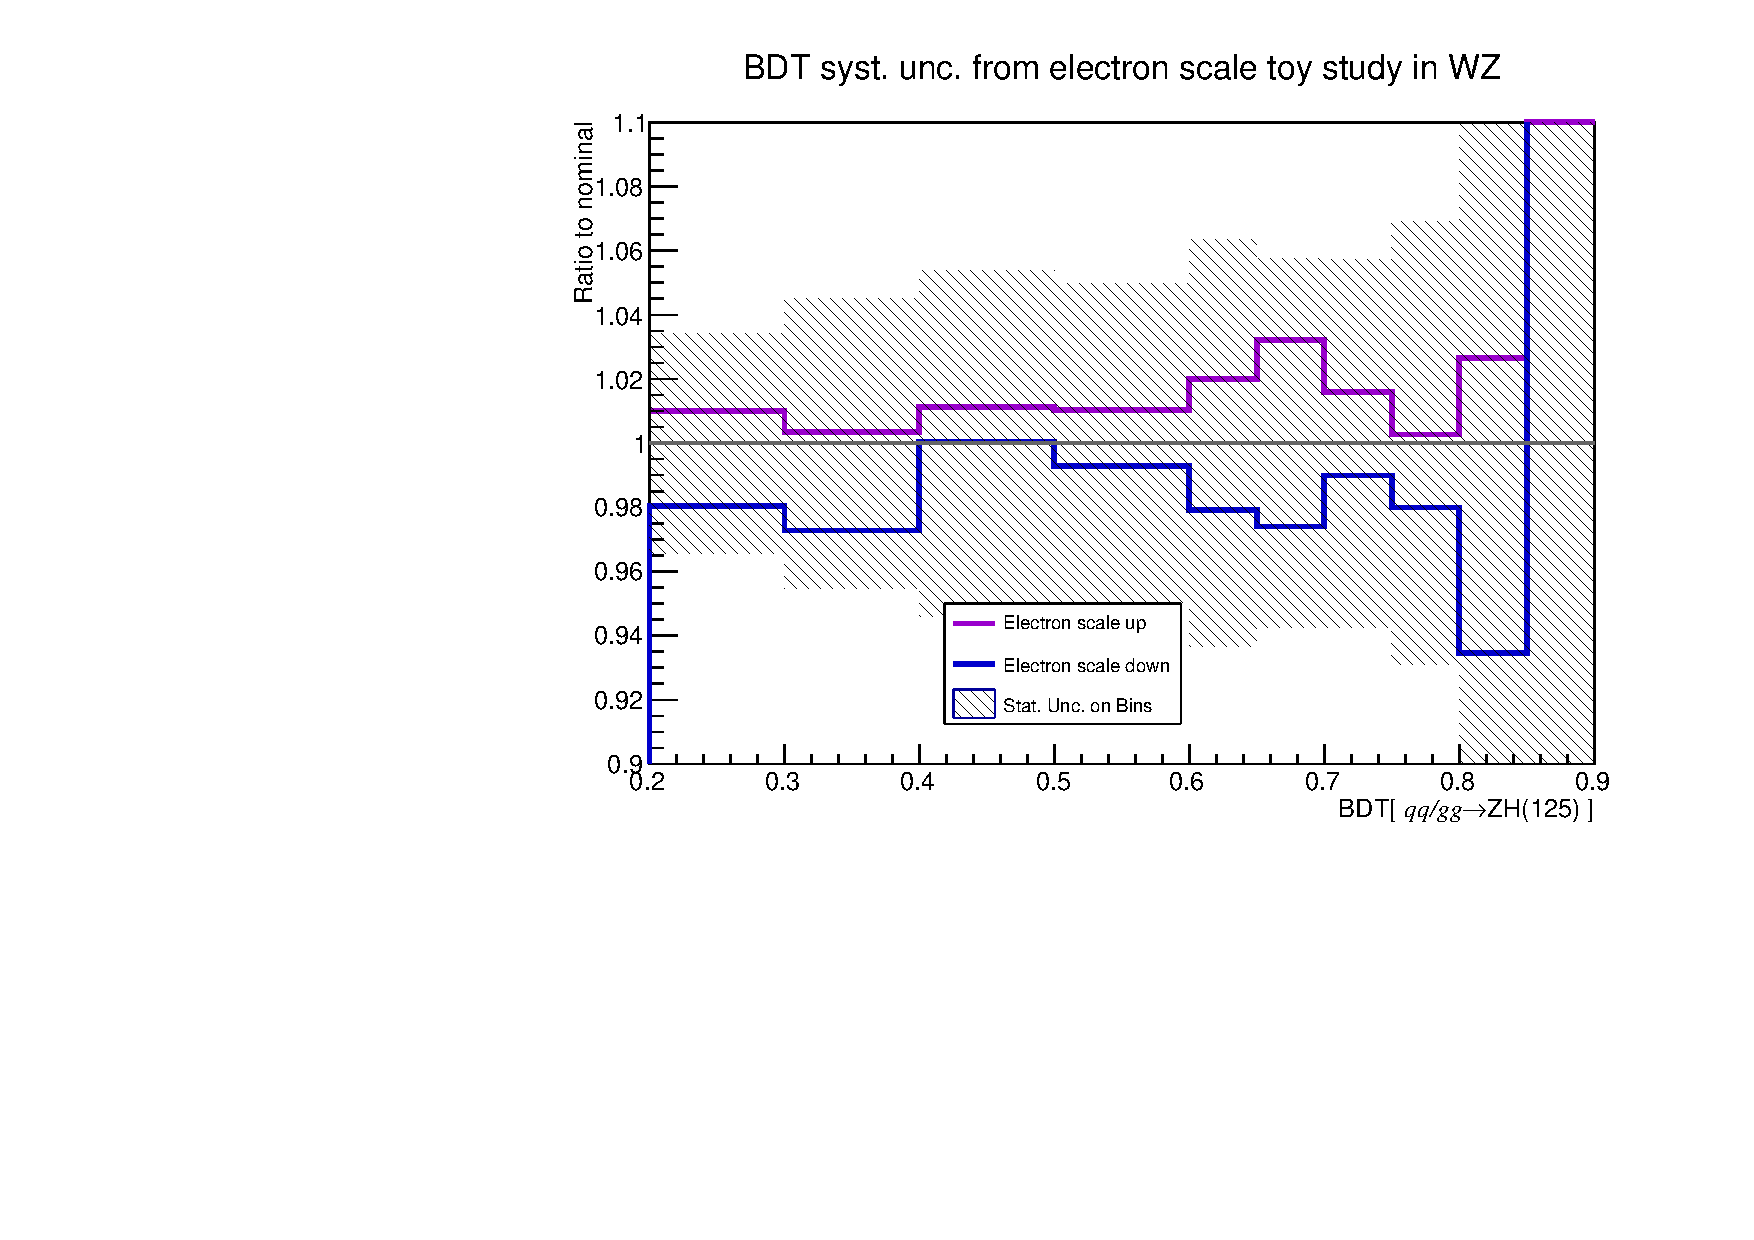
\includegraphics[width=0.48\textwidth]{figures/syst_BDT_WZ_toys_electron.pdf}
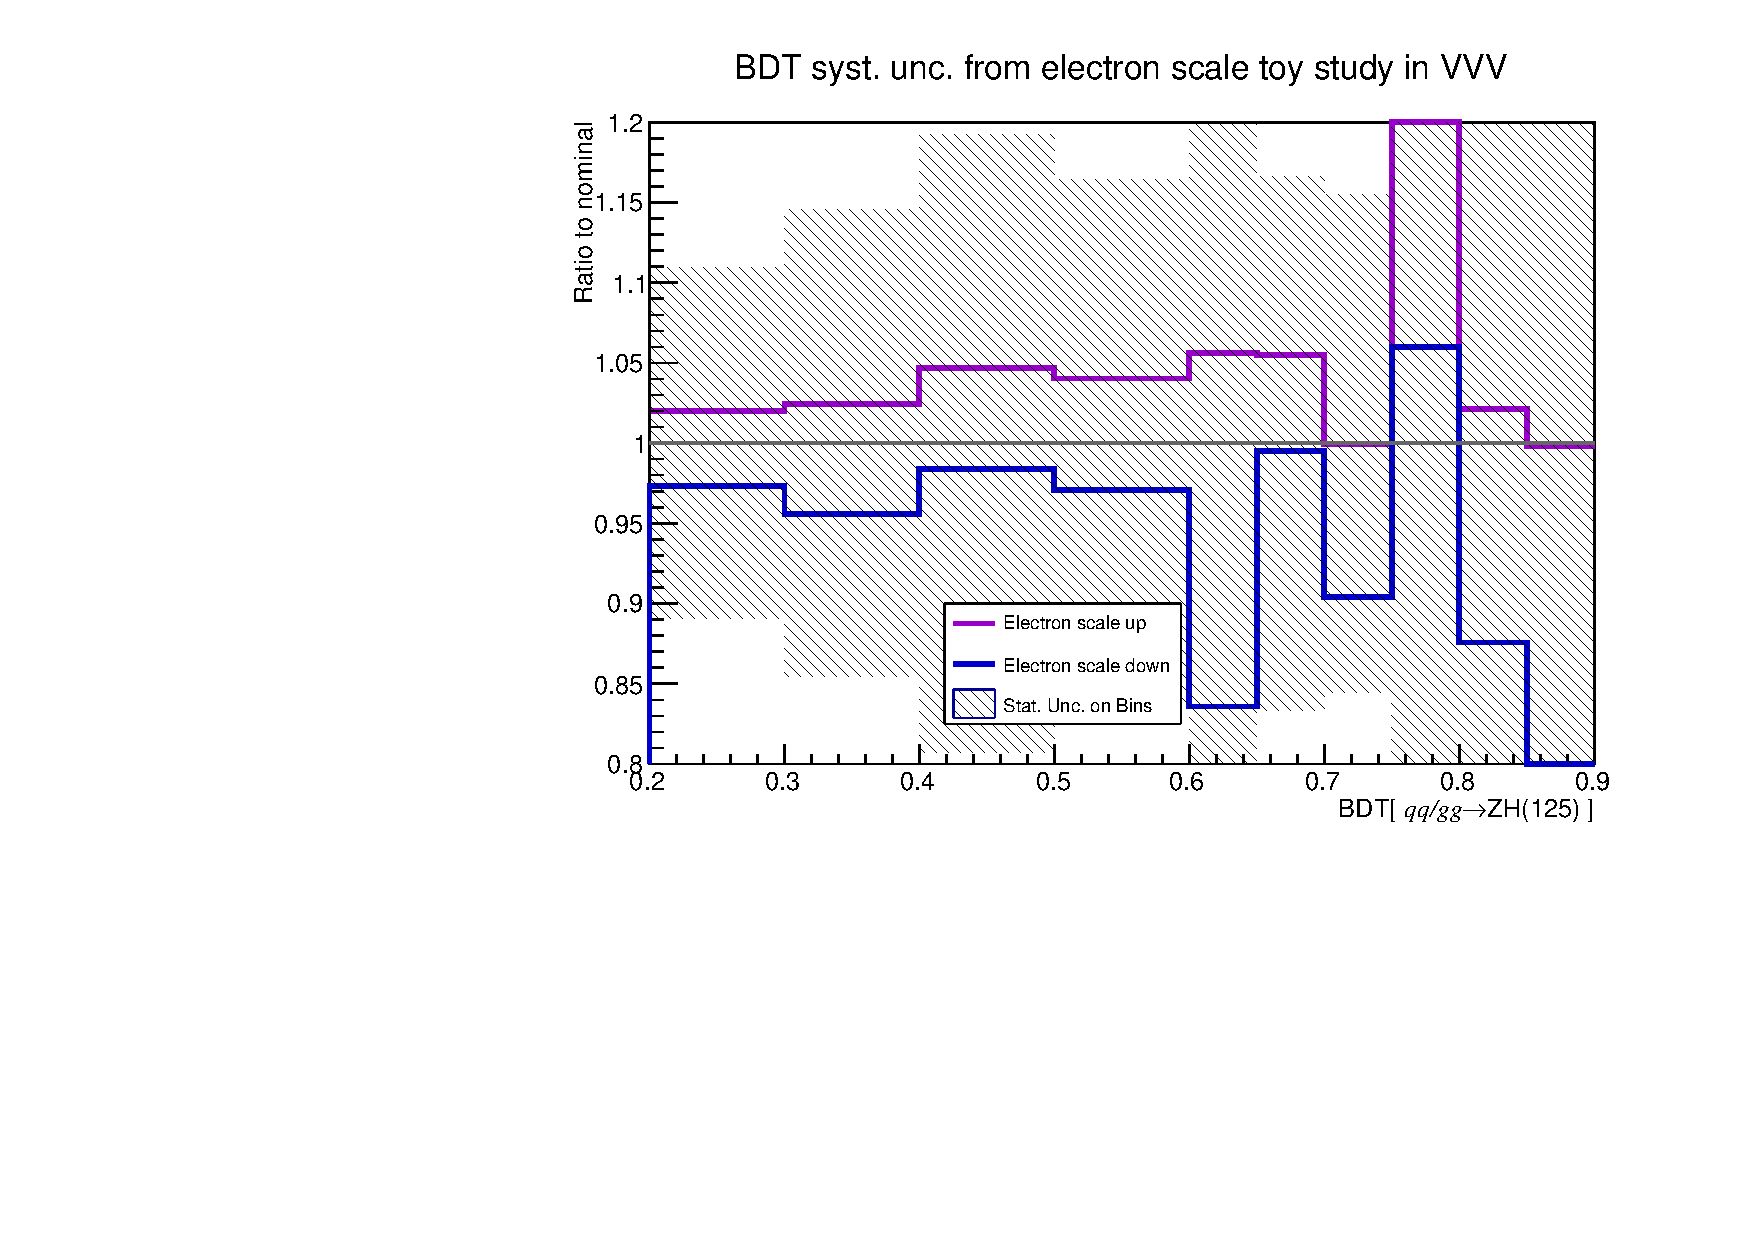
\includegraphics[width=0.48\textwidth]{figures/syst_BDT_VVV_toys_electron.pdf}
\caption{Uncertainty shapes calculated from the toy method for the electron scale.}
\label{fig:bdt_electron_scale}
\end{center}
\end{figure}

\begin{figure}[htbp]
\begin{center}
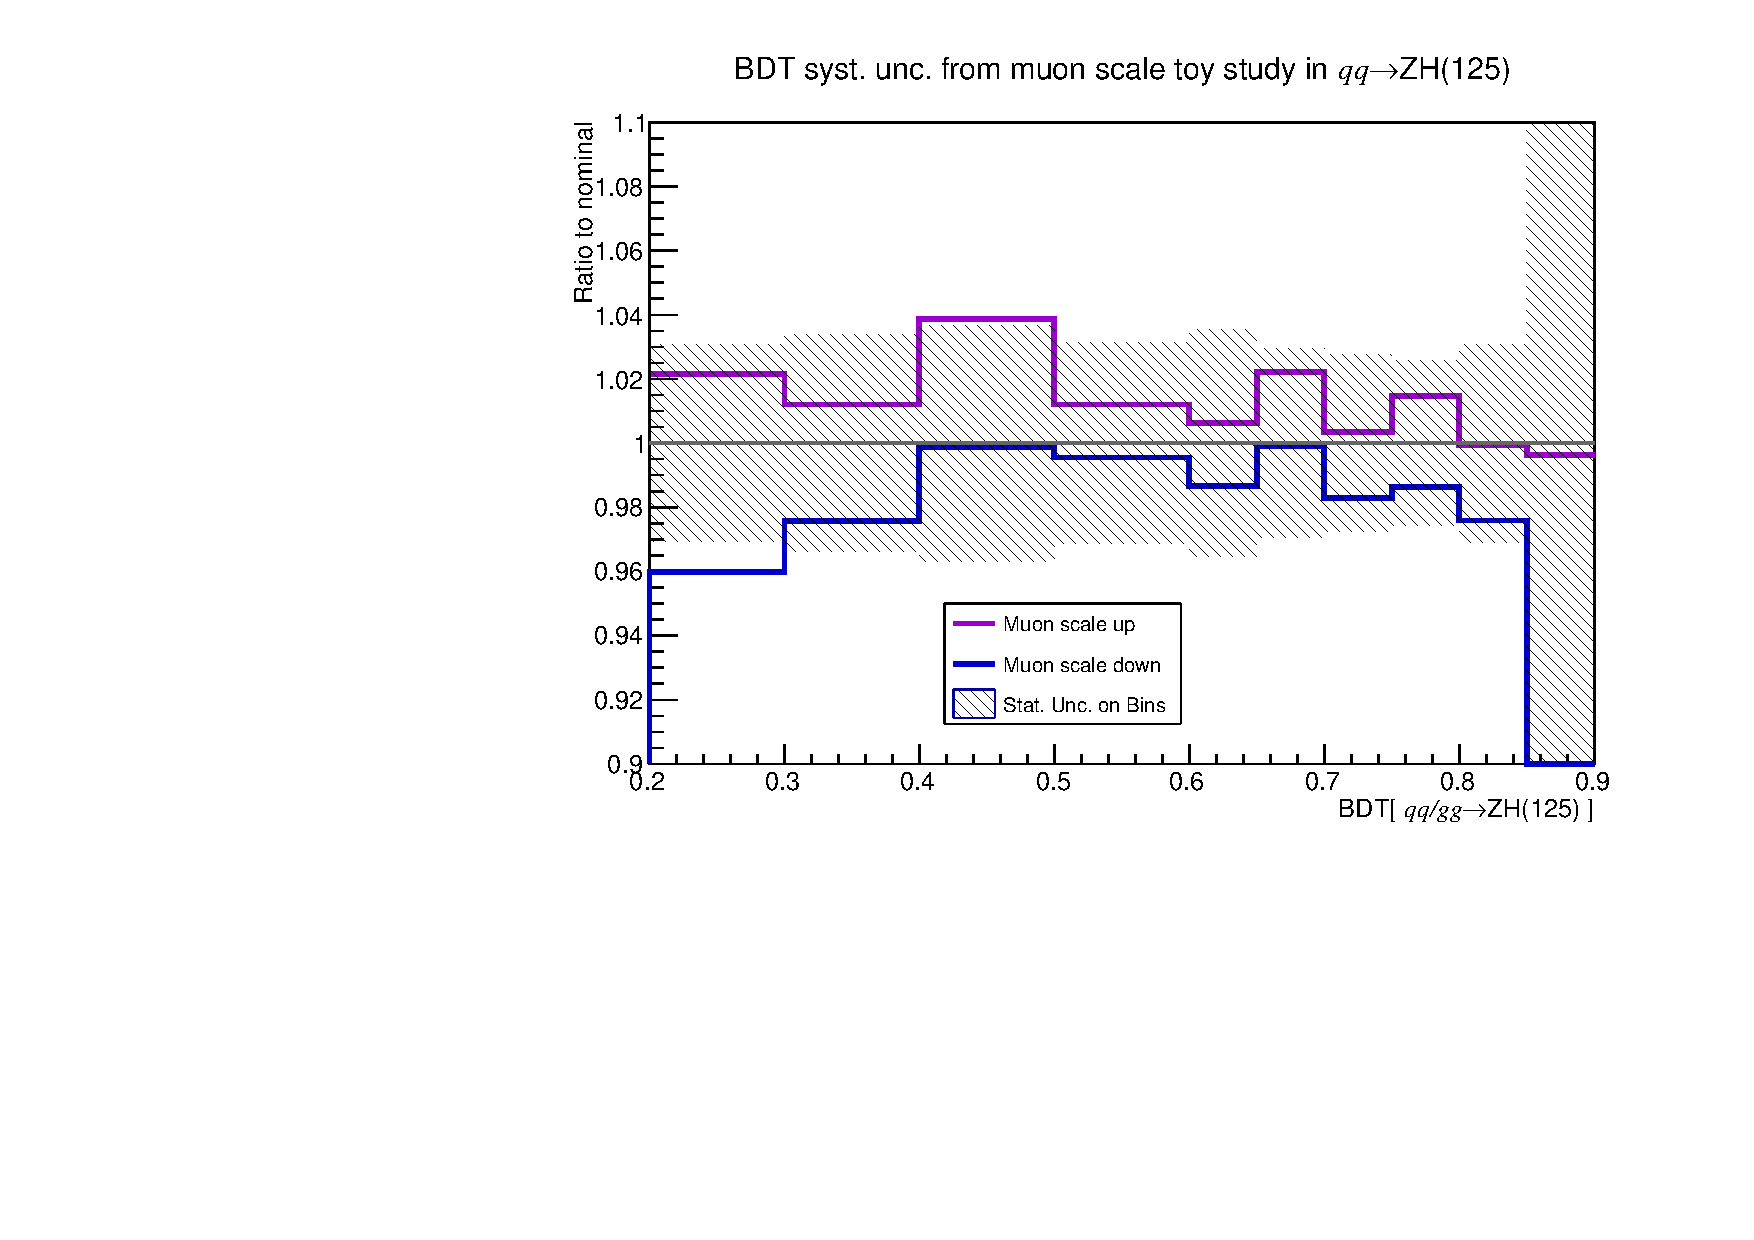
\includegraphics[width=0.48\textwidth]{figures/syst_BDT_ZH_hinv_sm_toys_muon.pdf}
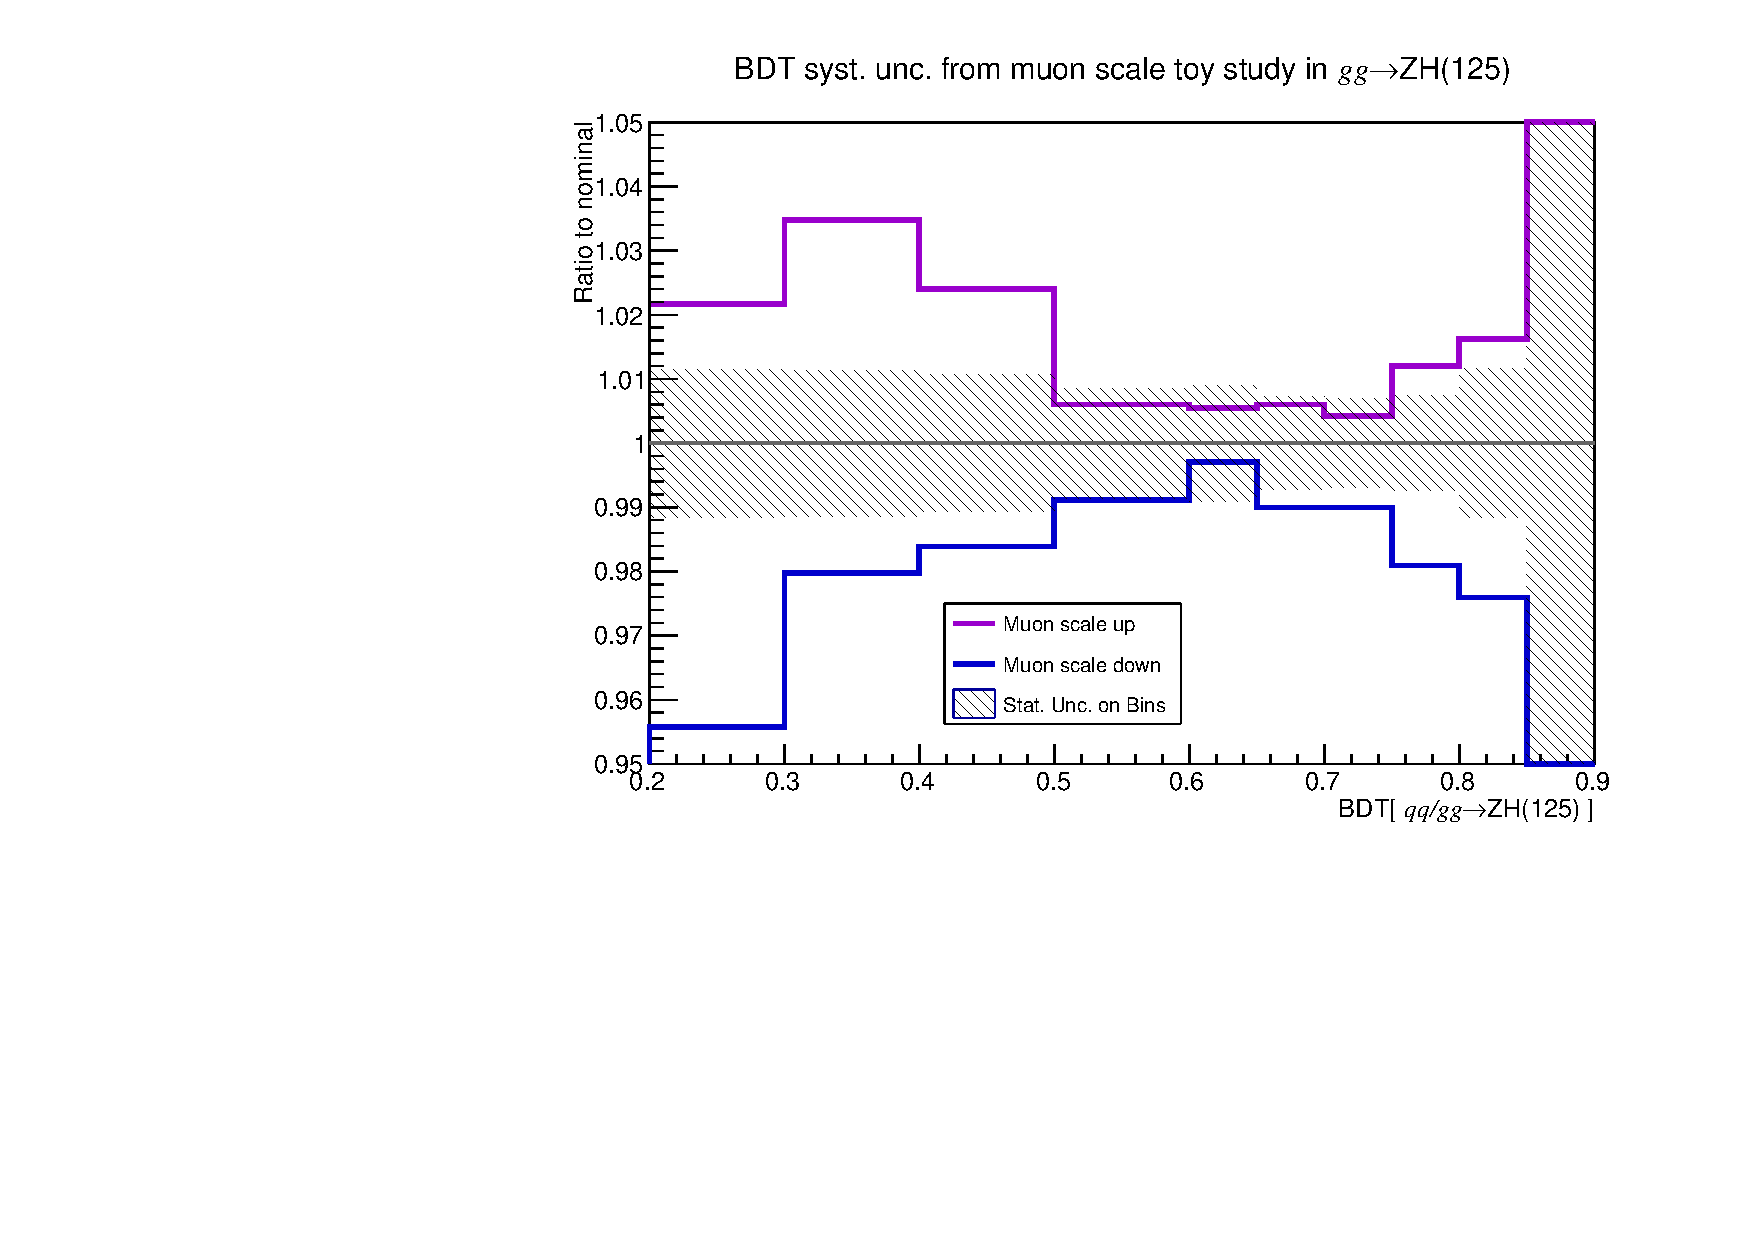
\includegraphics[width=0.48\textwidth]{figures/syst_BDT_ggZH_hinv_toys_muon.pdf}
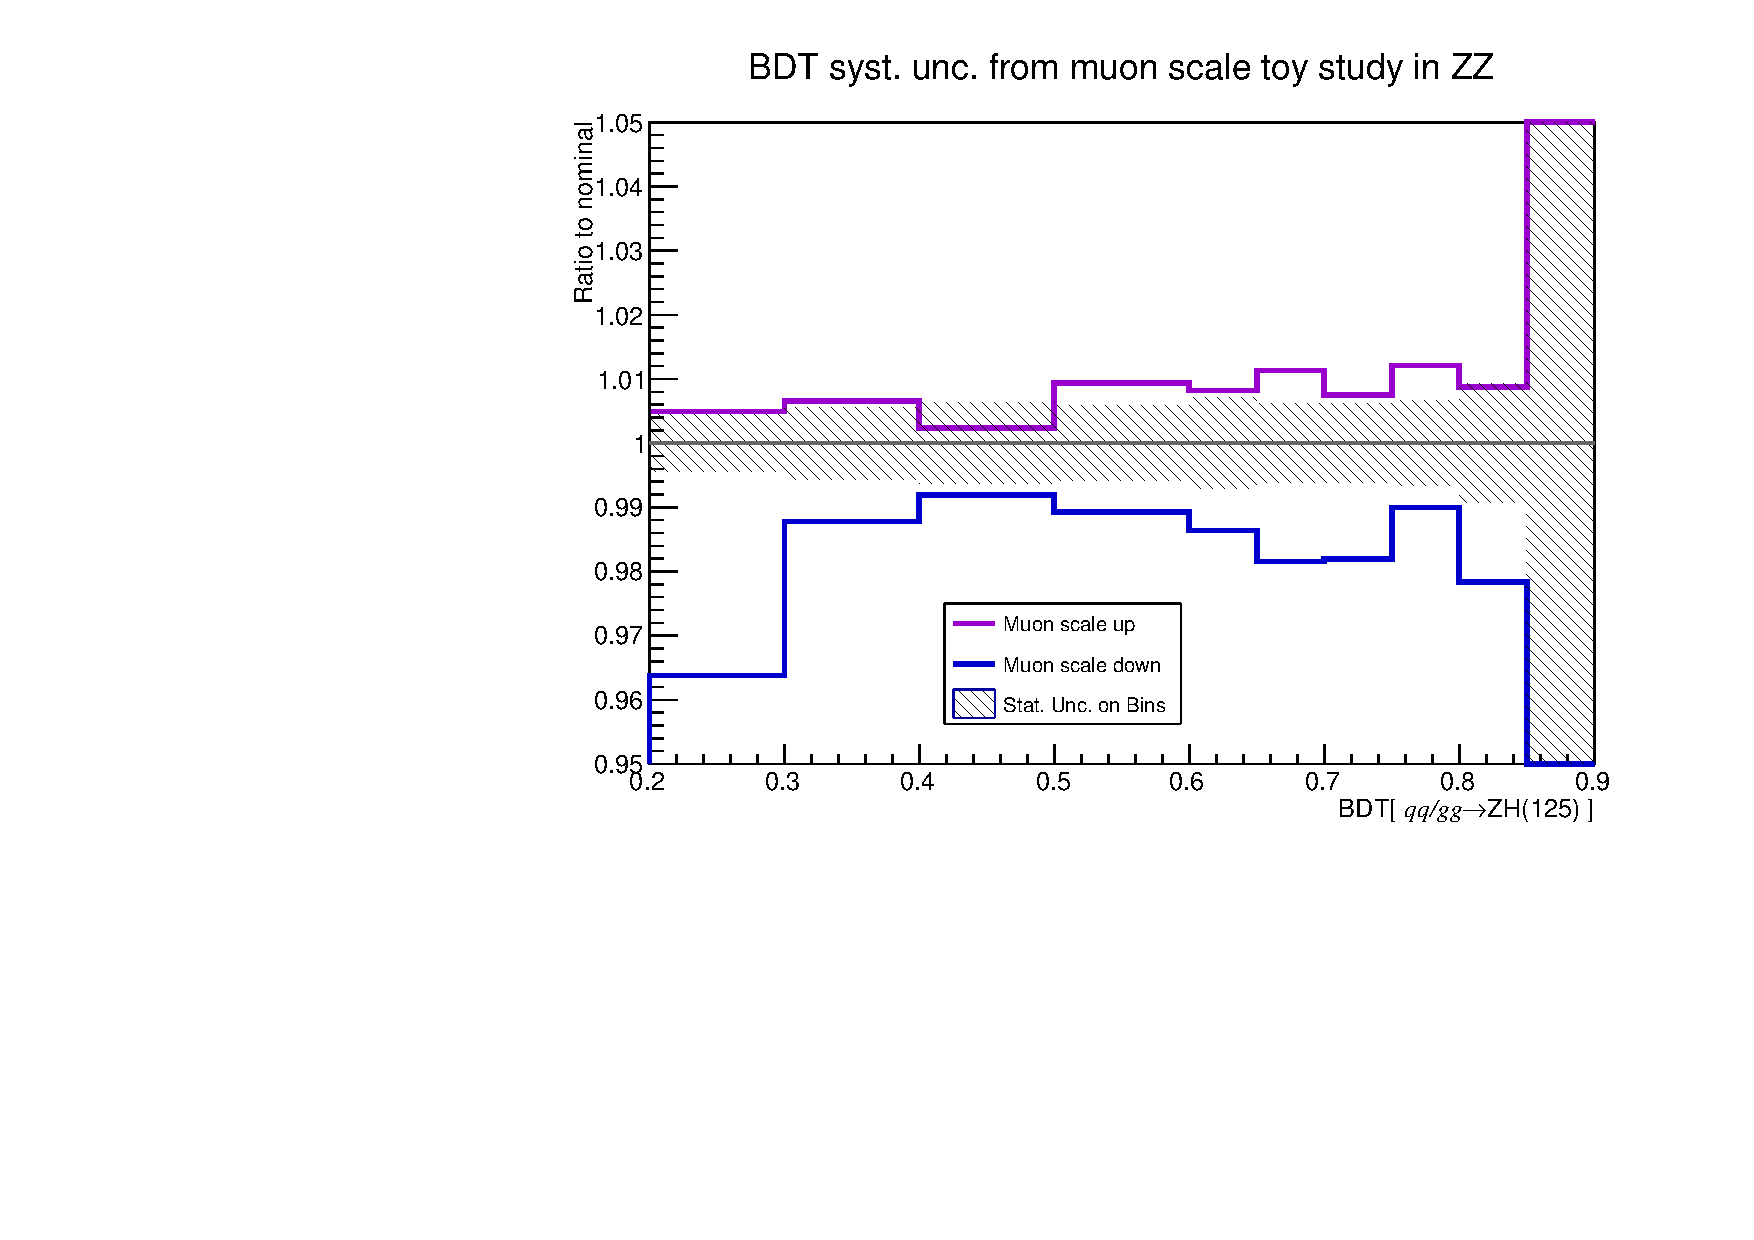
\includegraphics[width=0.48\textwidth]{figures/syst_BDT_ZZ_toys_muon.pdf}
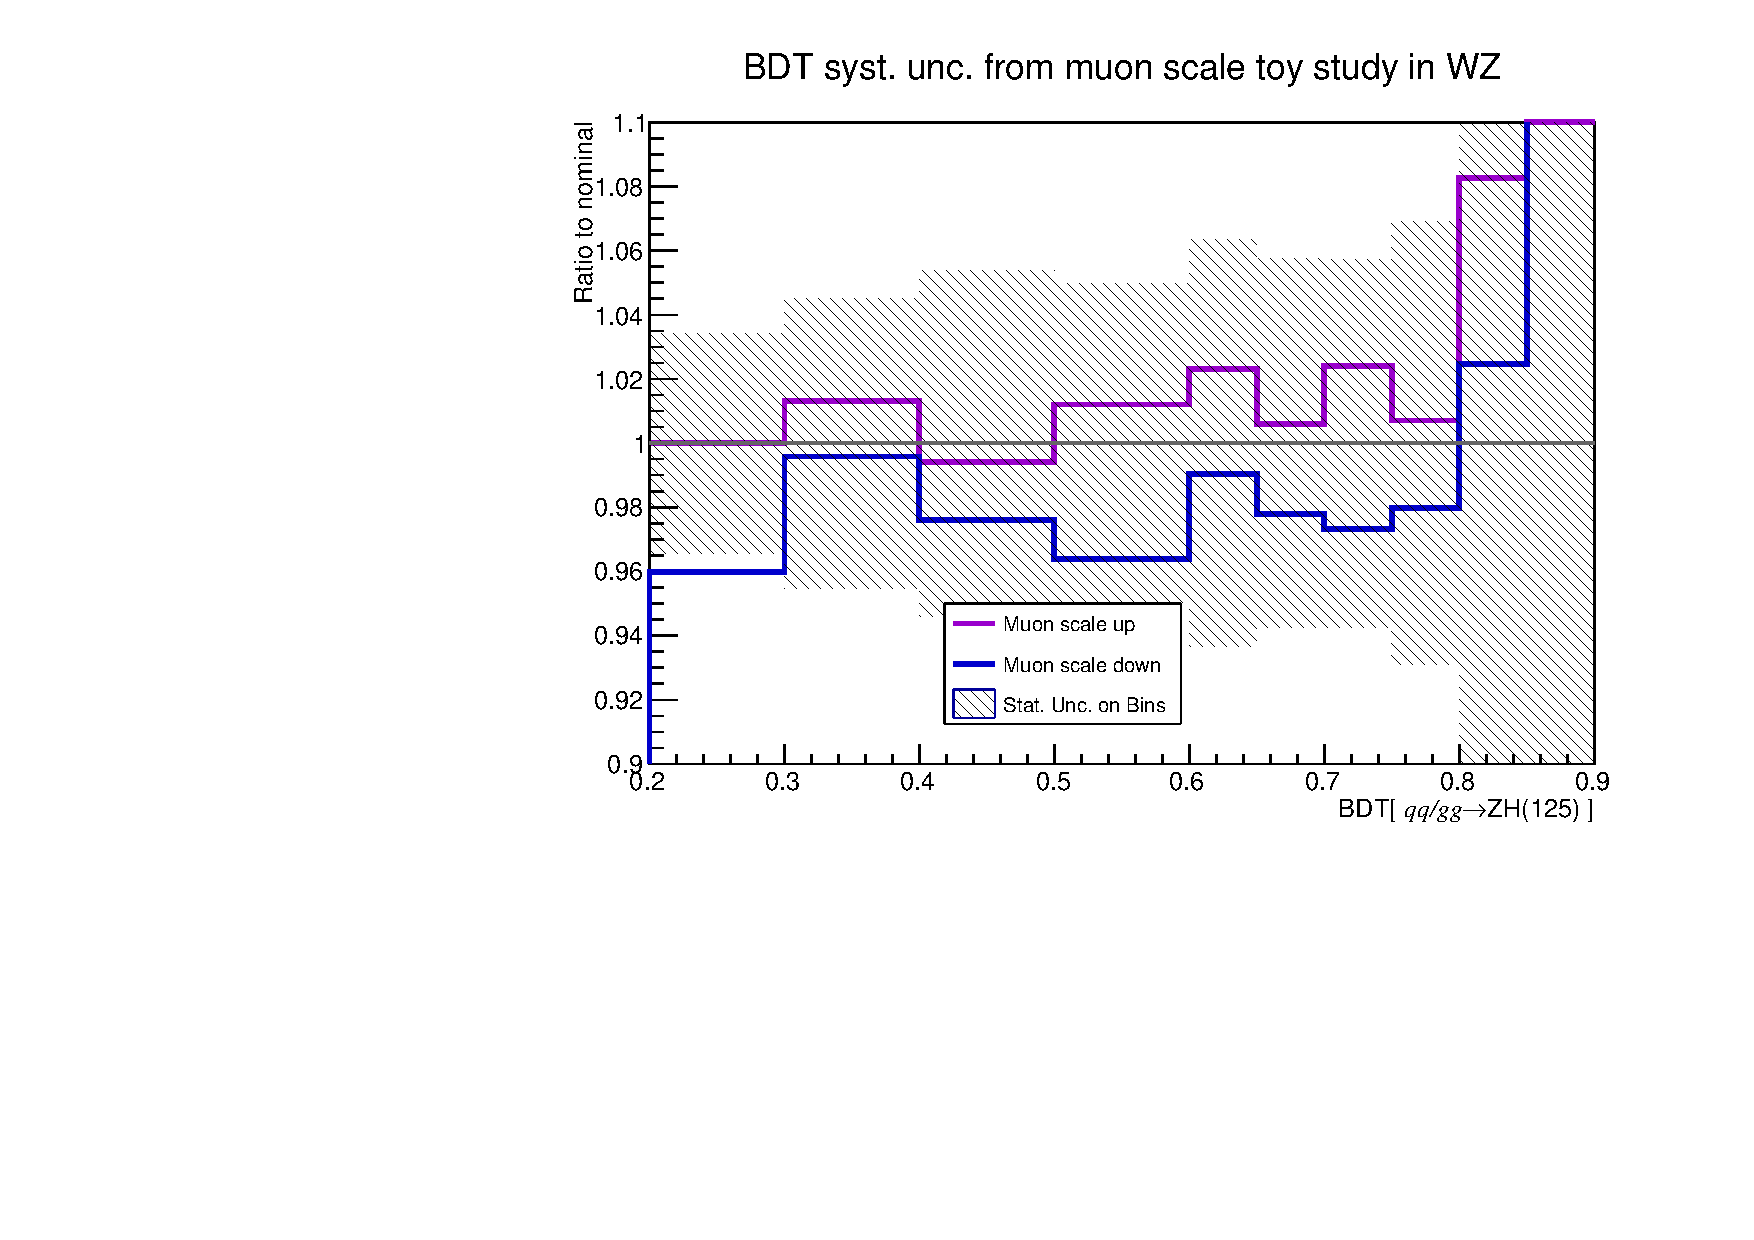
\includegraphics[width=0.48\textwidth]{figures/syst_BDT_WZ_toys_muon.pdf}
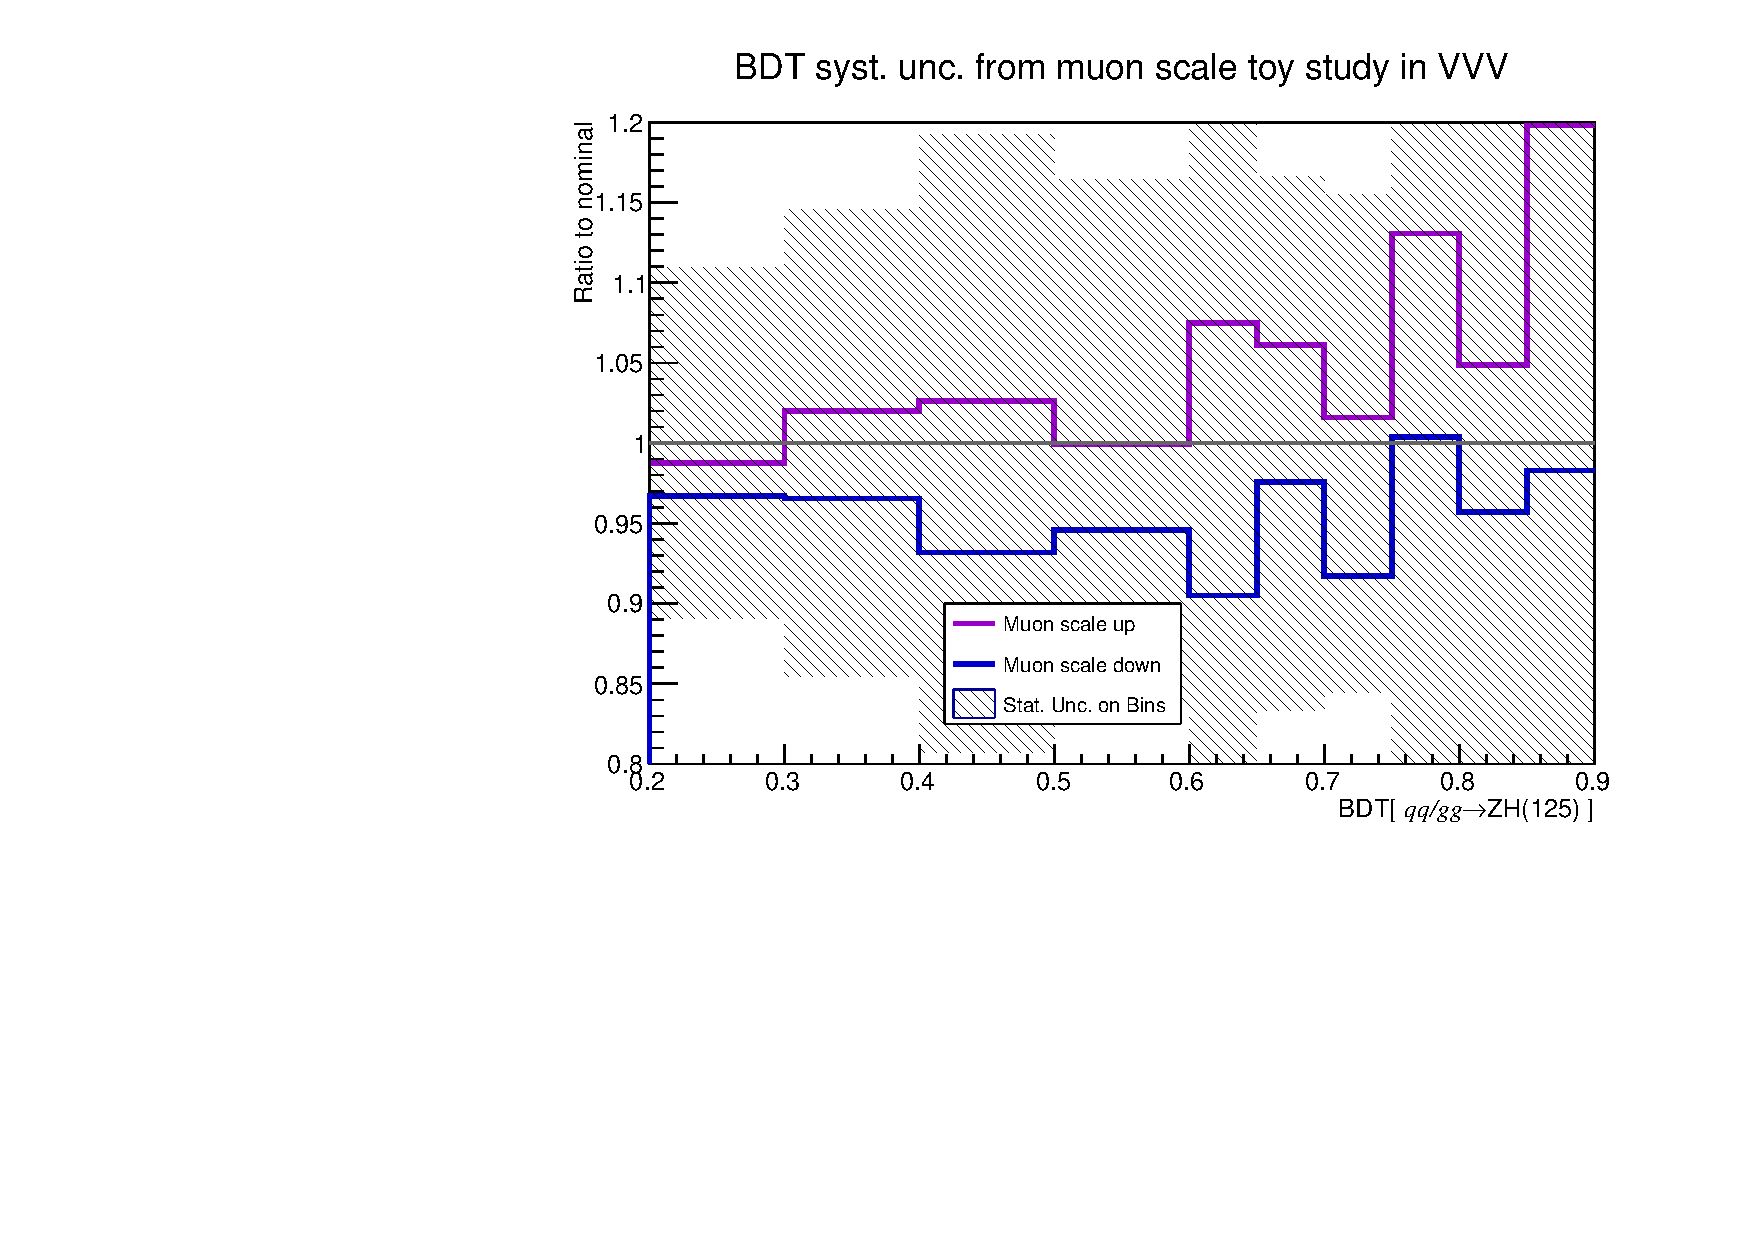
\includegraphics[width=0.48\textwidth]{figures/syst_BDT_VVV_toys_muon.pdf}
\caption{Uncertainty shapes calculated from the toy method for the muon scale.}
\label{fig:bdt_muon_scale}
\end{center}
\end{figure}

\begin{figure}[htbp]
\begin{center}
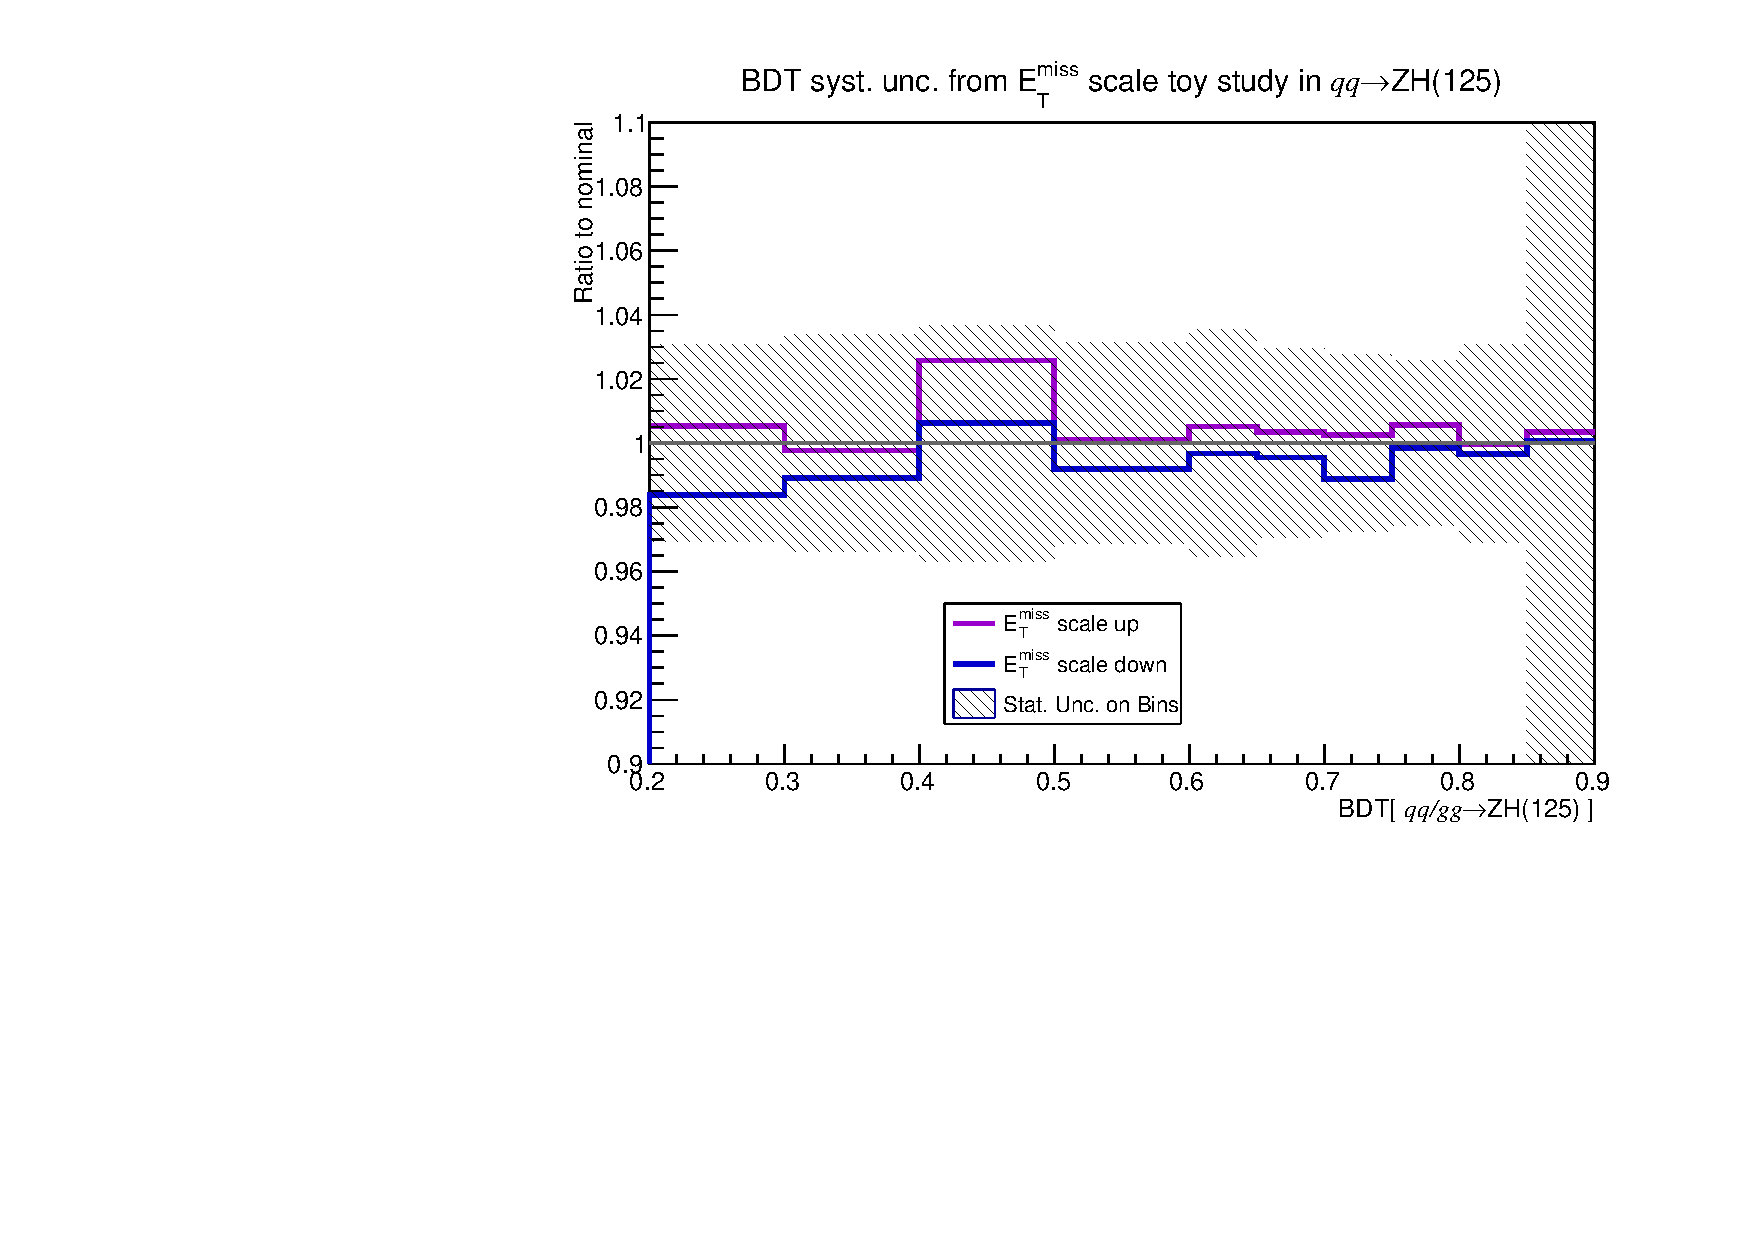
\includegraphics[width=0.48\textwidth]{figures/syst_BDT_ZH_hinv_sm_toys_MET.pdf}
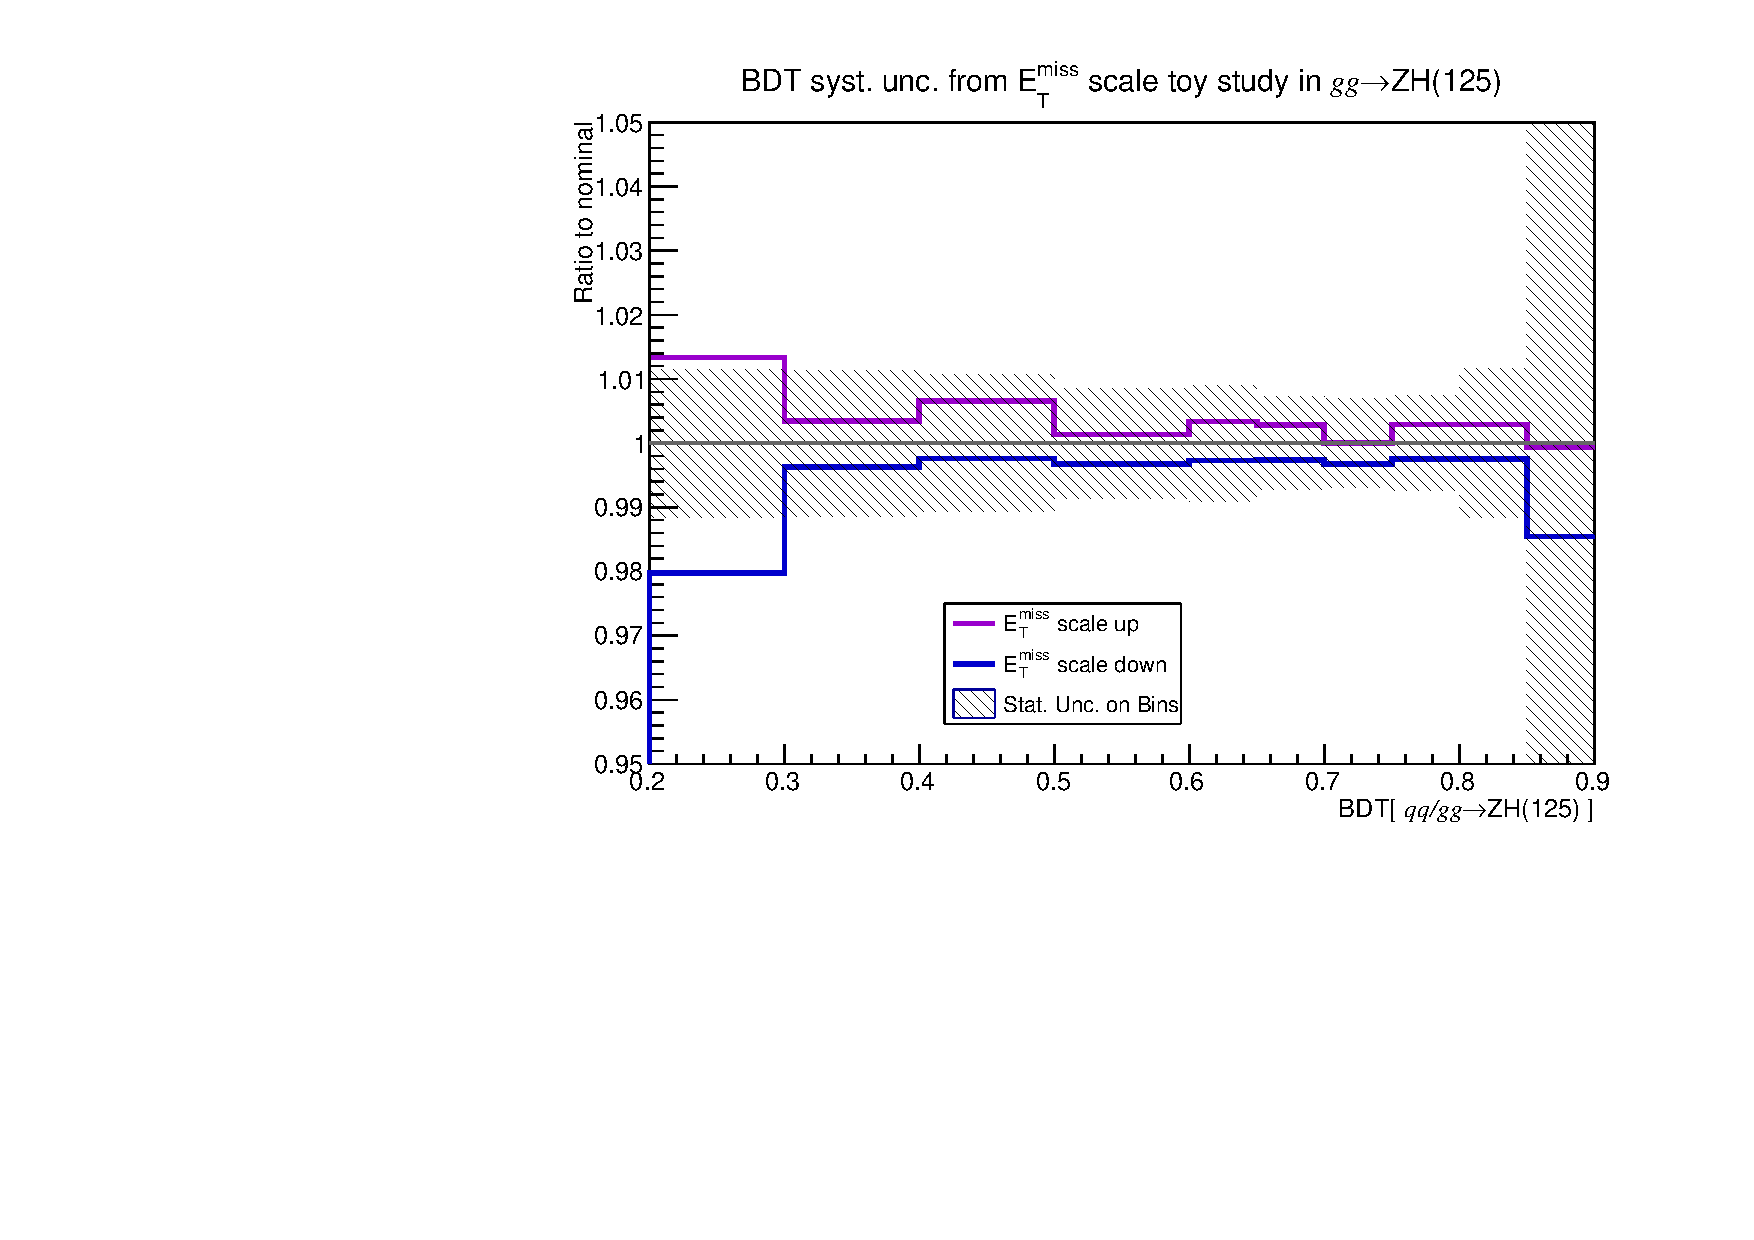
\includegraphics[width=0.48\textwidth]{figures/syst_BDT_ggZH_hinv_toys_MET.pdf}
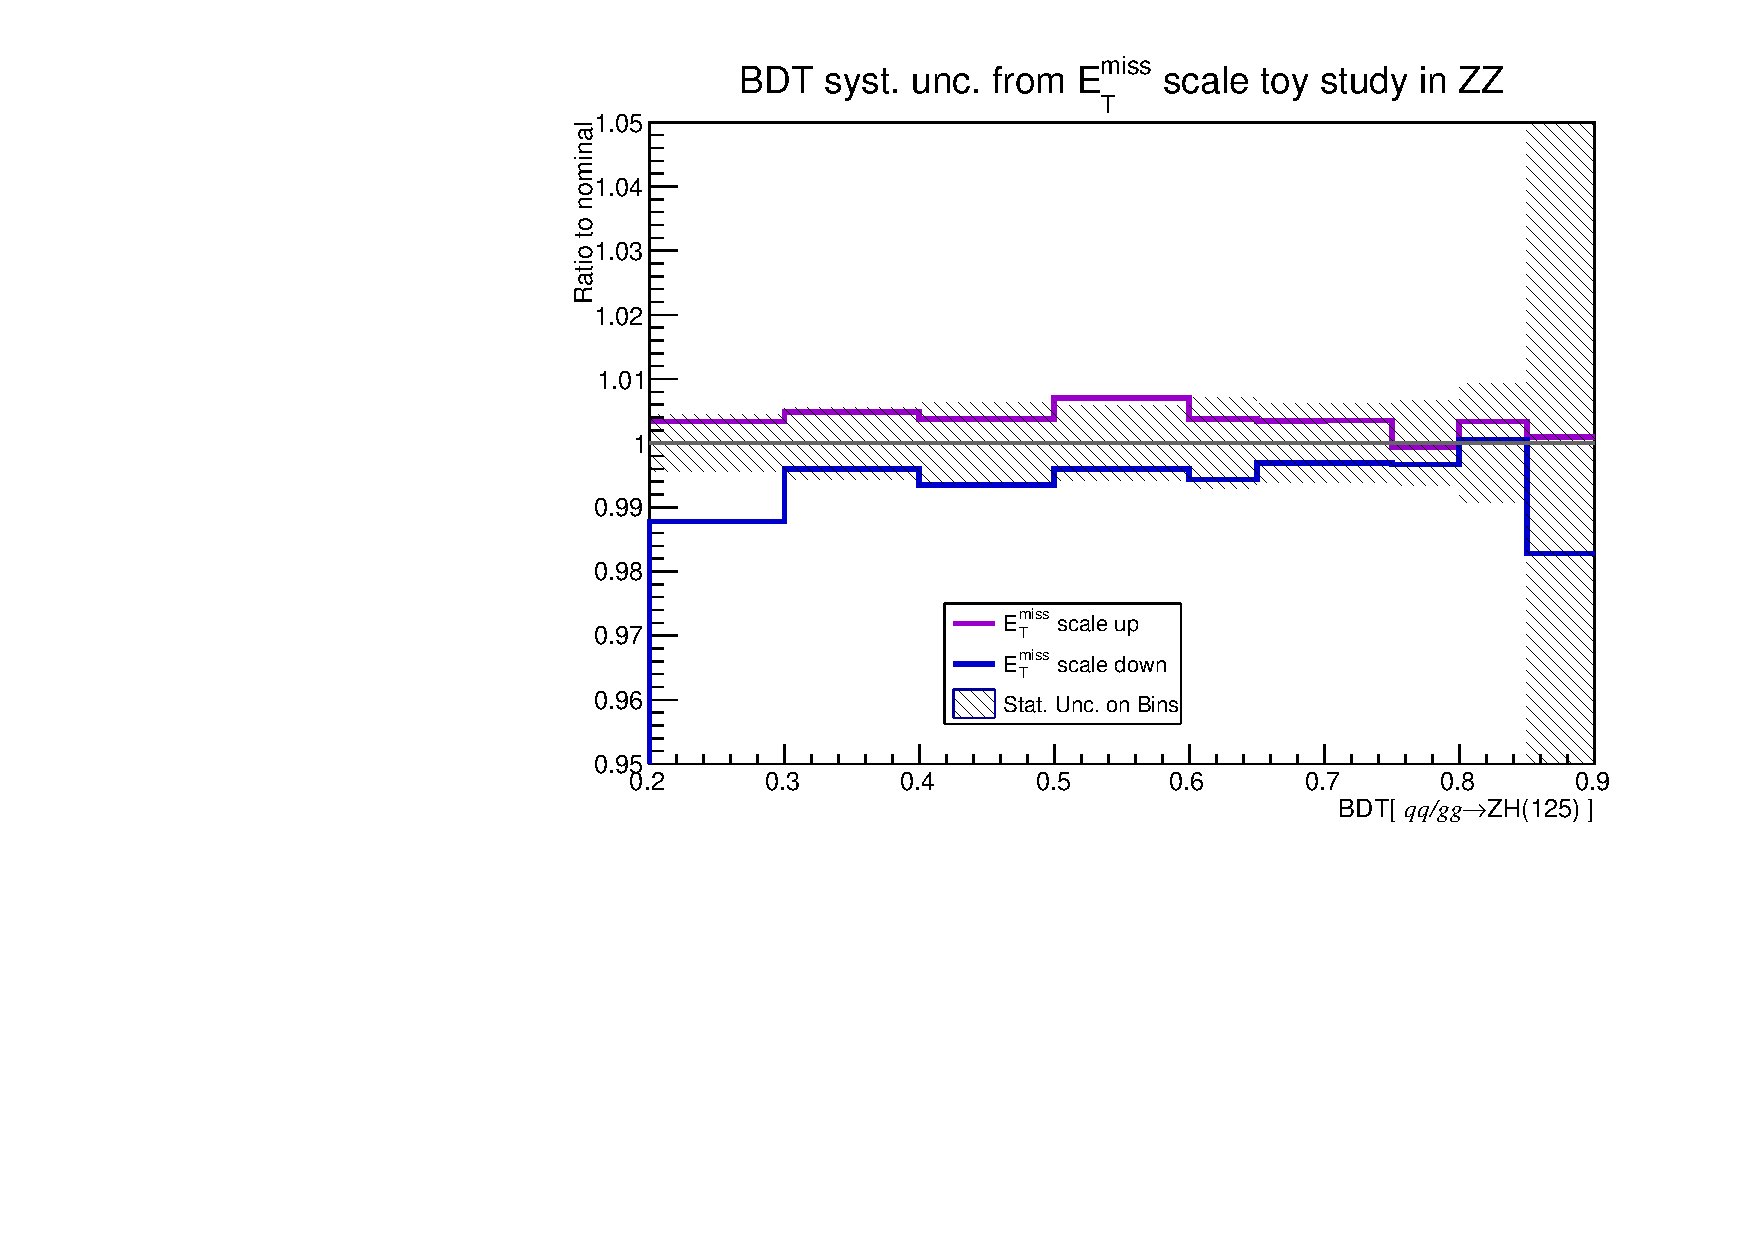
\includegraphics[width=0.48\textwidth]{figures/syst_BDT_ZZ_toys_MET.pdf}
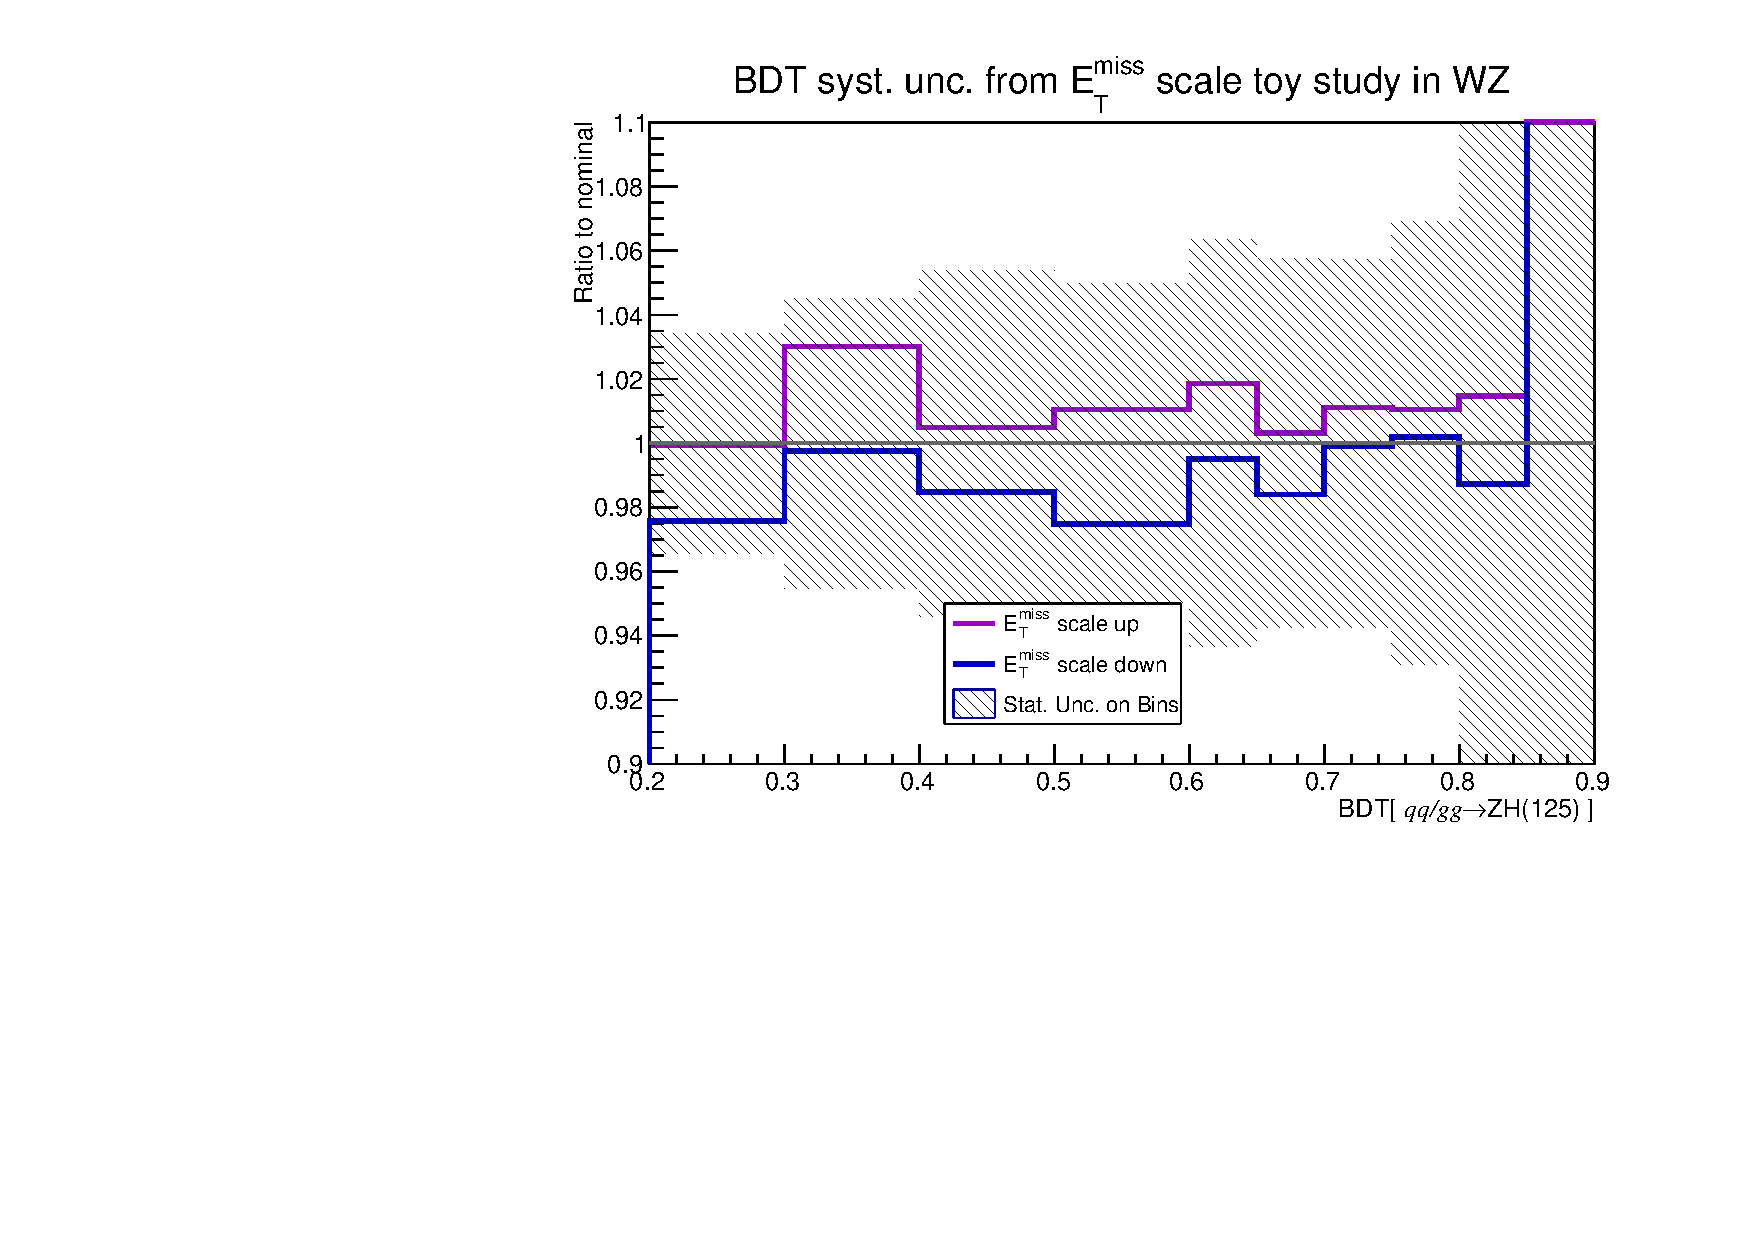
\includegraphics[width=0.48\textwidth]{figures/syst_BDT_WZ_toys_MET.pdf}
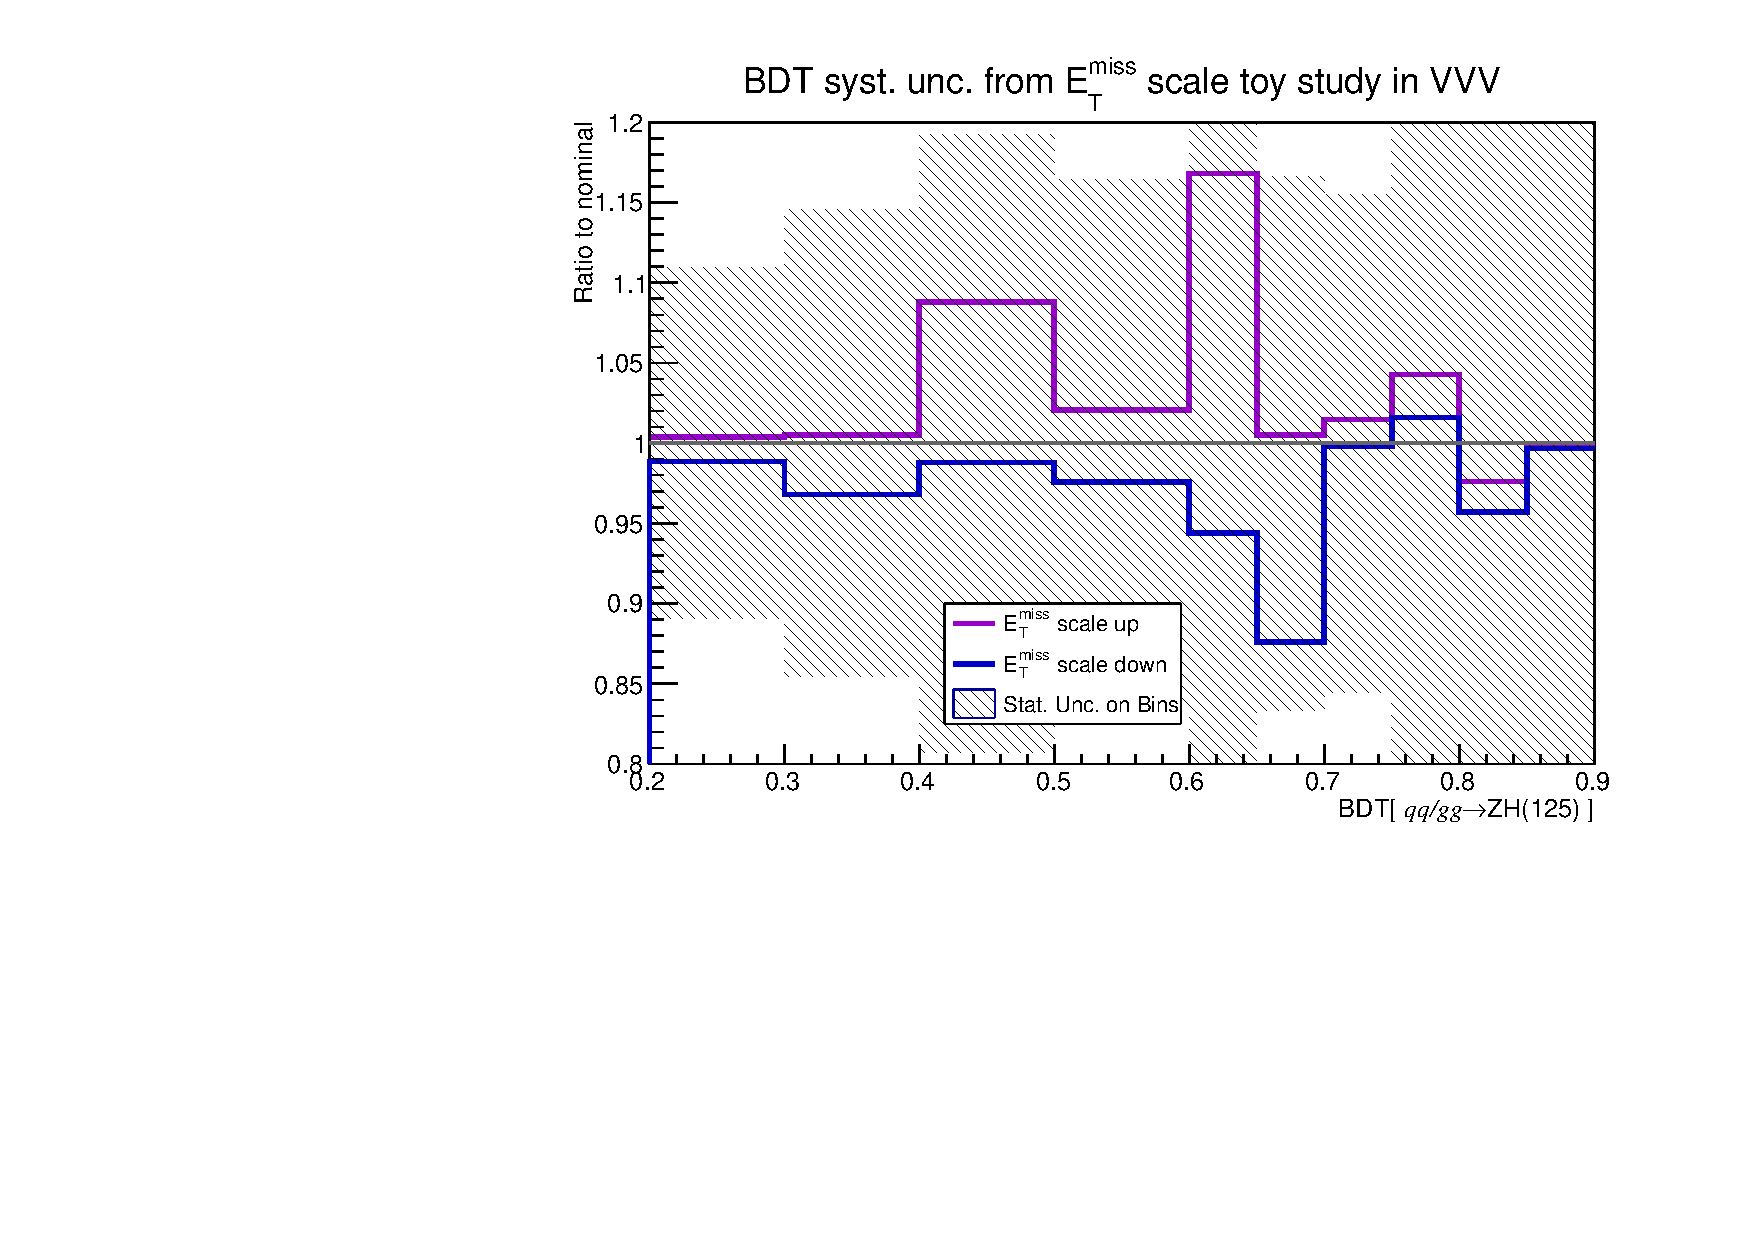
\includegraphics[width=0.48\textwidth]{figures/syst_BDT_VVV_toys_MET.pdf}
\caption{Uncertainty shapes calculated from the toy method for the \met due to the JES uncertainty.}
\label{fig:bdt_MET_scale}
\end{center}
\end{figure}


